\clearpage
%\begin{savequote}[8cm]
%\textlatin{Neque porro quisquam est qui dolorem ipsum quia dolor sit amet, consectetur, adipisci velit...}
%
%There is no one who loves pain itself, who seeks after it and wants to have it, simply because it is pain...
%  \qauthor{--- Cicero's \textit{de Finibus Bonorum et Malorum}}
%\end{savequote}

\chapter{\label{ch:5-cpfit}Fits for \CP observables in two- and four-body decays} 

%\minitoc

In this section the \CP observables are measured by performing an extended maximum likelihood fit to \btodkst candidates in data simultaneously for each \Dz decay mode for both \Bp and \Bm decays. This fit is referred to in this thesis as the \CP fit. The setup of the \CP fit is outlined in Section \ref{sec:cpfit:setup}, followed by the fit results in Section \ref{sec:cpfit:results}. Section \ref{sec:systematics} outlines the systematic uncertainties and the results of the \CP observables are summarised in Section \ref{sec:cpfit:summary}.

\section{Setup of \CP fit}
\label{sec:cpfit:setup}

The \CP fit to data is performed on the invariant mass of \btodkst candidates. A simultaneous fit strategy is employed to fit each of the \Dz decay modes as well as two bins of \B charge (\Bp and \Bm), two bins of \KS reconstruction type (LL and DD) and two bins of data type (\runone and \runtwo), resulting in 56 bins in total. The parameters extracted from this simultaneous fit are the \CP observables, namely \Akpi, \Akk, \Apipi, \Rkk, \Rpipi, \Rptwo, \Rmtwo, \Akpipipi, \Apipipipi, \Rpipipipi, \Rpfour and \Rmfour, which relate to the physics parameters of interest as shown in Equations \ref{exp_Acp} - \ref{exp_R4pi}.

The simultaneous fit extracts the \CP observables directly, rather than measuring the pure yields and indirectly converting them into the \CP observables, as described in Section \ref{sec:cpfit:likelihood}. The strategy to extract the \CP observables directly avoids the need to deal with combining results from different categories, which is complicated due to the many correlations between the variables. This strategy also leaves fewer fit parameters to be dealt with. The reason for performing the fit simultaneously is that the \CP observables being measured relate to the ratios of yields in different \Dz modes and different \B meson charges, therefore it is necessary to perform a fit that includes separate data samples associated with each of the modes and charges. Additionally, some shape parameters are found to be different in the different in different bins of \KS reconstruction type and data-taking period, and a simultaneous fit allows these differences to be easily dealt with. 

\subsection{Additional background component in \kk mass spectrum}
\label{sec:cpfit:Lb2LcKst}

The mass fit model described in Section \ref{sec:massfit} is used to model all \Dz modes in the \CP fit, however, there is an additional source of background included in the \kk model that does not occur in the other modes. This background comes from the decay \decay{\Lb}{\Lc(p\Km\pip)\Kstarm}, where the proton is misidentified as a kaon and the \pion is missed in the reconstruction. The decay mode \decay{\Lc}{p\Km\pip} accounts for over 6\% of the \Lc branching fraction~\cite{PDG2016}, whereas \Lc decays that may contribute as background to the other \Dz decay modes, e.g. \decay{\Lc}{p\pim\pip}, are suppressed by an order of magnitude. Additionally, the probability of incorrectly identifying a proton as a kaon is much larger than a pion, as they are much closer in mass. Other backgrounds that involve the proton being missed in the reconstruction are not considered as the reconstructed \Bm mass would not fall in the range under consideration. Therefore, for this family of decay modes, only the \decay{\Lb}{\Lc(p\Km\pip)\Kstarm} background, contributing to the \kk decay model, is considered.

The shape used to model this \decay{\Lb}{\Lc(p\Km\pip)\Kstarm} contribution is a Cruijff PDF, defined as,
\begin{equation}
  P_{\Lambda}(m; \mu,\sigma_L,\sigma_R,\alpha_L,\alpha_R)=
\begin{cases}
    \mathcal{K}_{L} exp \left( -\frac{(m-\mu)^2}{2\sigma_L^2 + \alpha_L(m-\mu)^2} \right) ,     & \text{if } m-\mu < 0, \\
    \mathcal{K}_{R} exp \left( -\frac{(m-\mu)^2}{2\sigma_R^2 + \alpha_R(m-\mu)^2} \right) ,     & \text{otherwise.}
\end{cases}
\label{Cruijff}
\end{equation}%
where $\mu$ is the peak position, $\sigma_{L,R}$ is the width on the left and right sides of the peak, $\alpha_{L,R}$ is a modification constant and $\mathcal{K}_{L,R}$ are the normalisation constants required for the PDF. Due to reasons relating to timing and speed of generation, a simulated sample of \decay{\Lc}{p\Km\pip} events is not available. Therefore, the parameters of the PDF are taken from a maximum likelihood fit to a simulated sample of \decay{\Lb}{\Lc\Km} events reconstructed as \decay{\Bm}{\D\Km} events; this PDF is expected to be similar to one taken from a \decay{\Lc}{p\Km\pip} sample, and any uncertainty in the shape is accounted for as a systematic uncertainty, described in Section \ref{sec:systematics}.

A maximum likelihood fit, as described in Section \ref{sec:massfit:likelihood}, is performed to the \Bm mass spectrum of the simulated sample. This fit is shown in Figure \ref{Lbfit}, where it can be seen that the reconstructed \Bm mass falls between 4800 and 5500 \mevcc. The results from this fit are shown in Table \ref{fitresultsLb}. All the values for the shape parameters are fixed in the simultaneous fit to the values in Table \ref{fitresultsLb}.

\begin{figure}[h]
\centering
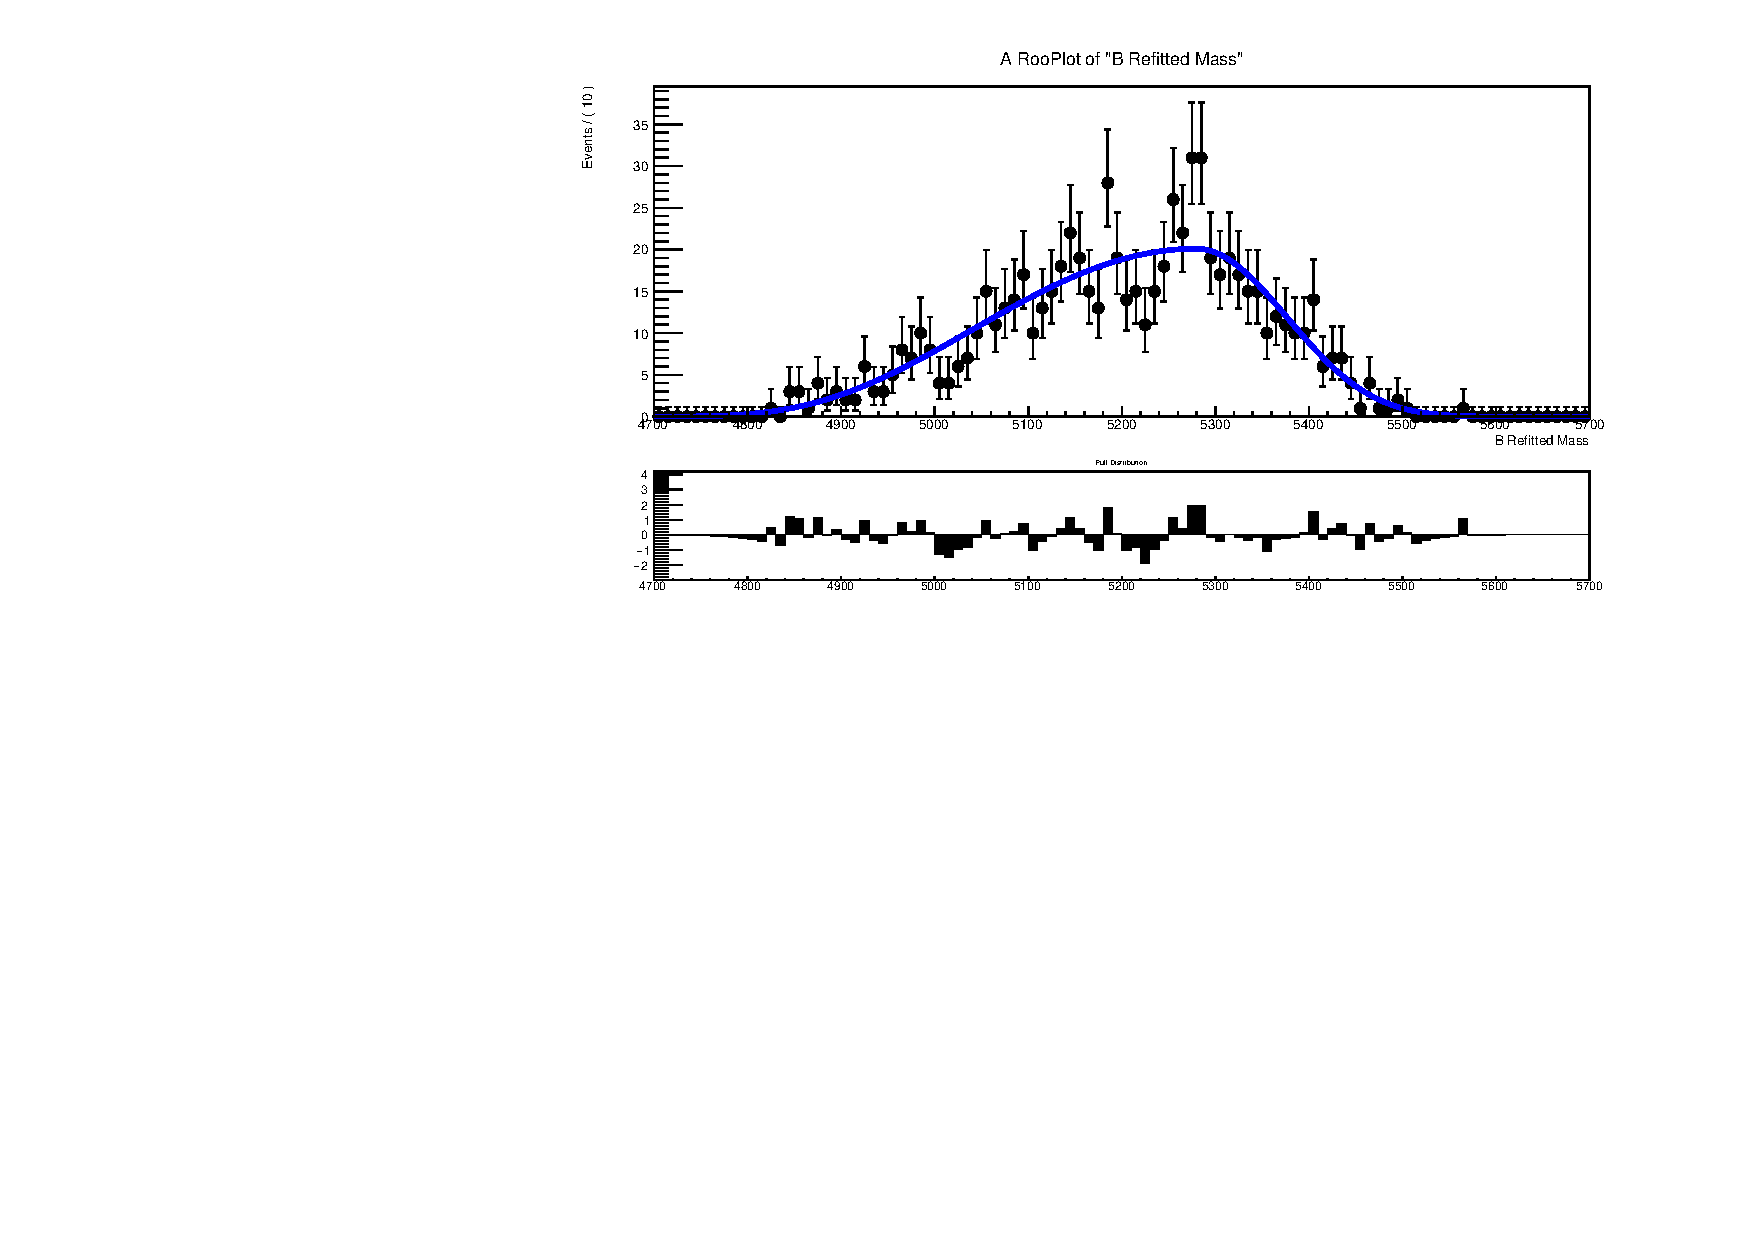
\includegraphics[width=0.7\linewidth]{figures/backgrounds/Lb2LcKst.pdf}
\caption{Maximum likelihood fit to distribution of simulated \decay{\Lb}{\Lc(p\Km\pip)\Km} sample using a Cruijff function, where the \pip is missed in reconstruction and the proton is misidentified as a kaon.}
\label{Lbfit}
\end{figure}

\begin{table}[h]
\centering
\begin{tabular}{cc}
\hline
Parameter & Value \\
\hline
$\mu$ & $5280 \pm 18$ \\
$\sigma_L$ & $221 \pm 26$ \\
$\sigma_R$ & $96 \pm 16$ \\
$\alpha_L$ & $-0.19 \pm 0.19$ \\
$\alpha_R$ & $-0.04 \pm 0.06$ \\
\hline
\end{tabular}
\caption{Shape parameters from a maximum likelihood fit to simulated \decay{\Lb}{\Lc\Km} events using a Cruijff PDF. These shape parameters are fixed in the \CP fit.}
\label{fitresultsLb}
\end{table}

The PDF is assumed to be the same in each \kk category of the \CP fit because there is such a low number of events that contribute to this background that the possible variations in the shape in the different categories has negligible effect on the results. The \decay{\Lb}{\Lc(p\kaon\pi)\Kstarm} yield as a fraction of the signal yield in the favoured \kpi mode, $f_{\Lambda}$, is allowed to vary in the simultaneous fit. This fractional yield is required to be the same for all fit categories.

%%%%%%%%%%%%%%%%%%%%%%%%
\subsection{Choice of fit range}
\label{sec:cpfit:range}	

Fixing the relative yields for the partially reconstructed shapes, as described in Section \ref{sec:massfit:partreco}, assumes that no \CP violation occurs, i.e. the relative yields for \Bm and \Bp are the same. This is a reasonable assumption for the favoured \kpi and \kpipipi decays considered in this section, where we do not expect \CP violation. However in the other \Dz final states, for example \pik, \CP violation is expected in the partially reconstructed background for which the \CP violation parameters are not known. Therefore, it is not possible make any constraints on the yield ratios in these modes. The fit that would result from fitting six individual yields with an order of magnitude less data would be unstable and this lack of constraint in the low mass region would lead to a large amount of freedom in the combinatorial, significantly affecting the precision of the signal yield. 

The overlap of the partially reconstructed and signal peaks is very small. There are a number of advantages to raising the lower range of the mass parameterisation up to 5230 \mev, which only removes 0.4\% of signal. The advantages include avoiding the need to fit the various partially reconstructed yields in each of the other \Dz decays modes, which is problematic due to expected \CP violation. Further benefits are that low level broad backgrounds, for example \decay{\Bm}{\D\Kstarm\piz} and \decay{\Bd}{\Kp\pim\pip\pim}, which may be present in the range 4900 - 5200 \mev do not need to considered as sources of systematics uncertainty. 

\subsection{Partially reconstructed yield in \CP fit}
\label{sec:cpfit:partrecoyields}

The modelling of the partially reconstructed background is described in detail in Section \ref{sec:massfit:partreco}. The low mass limit in the \CP fit is 5230\mevcc, which removes almost all of the partially reconstructed background. The shape and yield of the small amount of partially reconstructed background present in all \Dz decay mode categories above 5230 \mev is determined and fixed from the fits to data of the \kpi and \kpipipi decays, taking into account the smaller branching fractions of the \Dz decays. Table \ref{partrecofixedyields} shows the fixed values of the total partially reconstructed yield in the \CP fit. Due to the assumptions present in the initial fit, uncertainties in the yield and shape and possible asymmetries in distribution between \Bp and \Bm are evaluated as systematic uncertainties, as discussed in Section \ref{sec:systematics:partreco}. 

\begin{table}[h]
\centering
\begin{tabular}{c|cc|cc}
\hline
& \multicolumn{2}{c}{Run 1} & \multicolumn{2}{c}{Run 2} \\
& LL & DD & LL & DD \\
\hline
$K\pi$ & 0.55 & 1.03 & 1.18 & 1.35 \\
$KK$ & 0.060 & 0.112 & 0.116 & 0.131 \\
$\pi\pi$ & 0.019 & 0.034 & 0.041 & 0.049 \\
$\pi K$ & 0.008 & 0.012 & 0.017 & 0.016 \\
$K\pi\pi\pi$ & 0.34 & 0.52 & 0.55 & 1.31 \\
$\pi\pi\pi\pi$ & 0.031 & 0.045 & 0.050 & 0.122  \\
$\pi K\pi\pi$ & 0.004 & 0.006 & 0.007 & 0.014 \\
\hline
\end{tabular}
\caption{Partially reconstructed yields fixed in the \CP fit. The values show \Bp and \Bm combined; each of these numbers are divided equally between the \Bp and \Bm categories. Uncertainties for these values are O(10\%).}
\label{partrecofixedyields}
\end{table}

\subsection{Corrections to yield ratios}
\label{sec:cpfit:efficiencies}

The \CP observables related to the ratio of yields, \Rkk, \Rpipi, \Rptwo, \Rmtwo, \Rpipipipi, \Rpfour and \Rmfour, are physical quantities, which are independent of the detection and selection strategies employed. Therefore, in order to extract these \CP observables from the raw yield ratios, various efficiency corrections, taken from simulated signal samples, must be applied.

For the GLW modes, efficiency corrections are applied to the raw value of the yield ratios to extract \Rkk, \Rpipi and \Rpipipipi as shown in Equation \ref{effcorrectionglw2body} and \ref{effcorrectionglw4body}, where $\epsilon_{sel}$ and $\epsilon_{pid}$ are the selection and PID efficiencies respectively. Selection and PID efficiencies are considered separately as PID variables are poorly modelled in \lhcb simulation, therefore a separate method for determining PID efficiencies is used, as detailed in Section \ref{sec:cpfit:efficiencies:pid}. The values for these selection and PID efficiency corrections are given in Tables \ref{seleff} and \ref{pideff} respectively.

{\footnotesize
\begin{equation}
R_{hh} = \frac{N(\decay{\Bm}{\D(h^+h^-)\Kstarm})}{N(\decay{\Bm}{\D(\Km\pip)\Kstarm})} \times \frac{\BR(\decay{\Dz}{\Km\pip})}{\BR(\decay{\Dz}{hh})} \times \frac{\epsilon_{\text{sel}}(K\pi)}{\epsilon_{\text{sel}}(hh)} \times \frac{\epsilon_{\text{pid}}(K\pi)}{\epsilon_{\text{pid}}(hh)}
\label{effcorrectionglw2body}
\end{equation}
\begin{multline}
R_{\pi\pi\pi\pi} = \frac{N(\decay{\Bm}{\D(\pip\pim\pip\pim)\Kstarm})}{N(\decay{\Bm}{\D(\Km\pip\pim\pip)\Kstarm})} \times \frac{\BR(\decay{\Dz}{\Km\pip\pim\pip})}{\BR(\decay{\Dz}{\pi\pi\pi\pi})} \\ \times \frac{\epsilon_{\text{sel}}(K\pi\pi\pi)}{\epsilon_{\text{sel}}(\pi\pi\pi\pi)} \times \frac{\epsilon_{\text{pid}}(K\pi\pi\pi)}{\epsilon_{\text{pid}}(\pi\pi\pi\pi)} 
\label{effcorrectionglw4body}
\end{multline}}
As the final state in the ADS modes are almost identical to the corresponding charge favoured mode, the selection efficiencies that are common to both are assumed to cancel. There are only two differences between the selection for the ADS mode and the charge favoured mode; the tighter BDT selection for DD candidates and the double misidentification veto, which is only applied to the ADS mode. Equations \ref{effcorrectionads2body} and \ref{effcorrectionads4body} describe the efficiency corrections required to extract \Rptwo, \Rmtwo, \Rpfour and \Rmfour from the raw yield ratios, where $\epsilon_{bdt}$ and $\epsilon_{veto}$ are the BDT and veto efficiencies respectively. The values for these BDT and veto efficiency corrections are given in Tables \ref{bdteff} and \ref{vetoeff} respectively.

{\footnotesize
\begin{equation}
R^{\pm}_{K\pi} = \frac{N(\decay{\Bpm}{\D(\Kmp\pipm)\Kstarpm})}{N(\decay{\Bpm}{\D(\Kpm\pimp)\Kstarpm})} \times \frac{\epsilon_{\text{bdt}}(K\pi)}{\epsilon_{\text{bdt}}(\pi K)} \times \frac{1}{\epsilon_{\text{veto}}(\pi K)}
\label{effcorrectionads2body}
\end{equation}
\begin{equation}
R^{\pm}_{K\pi\pi\pi} = \frac{N(\decay{\Bpm}{\D(\Kmp\pipm\pimp\pipm)\Kstarpm})}{N(\decay{\Bpm}{\D(\Kpm\pimp\pipm\pimp)\Kstarpm})} \times \frac{\epsilon_{\text{bdt}}(K\pi\pi\pi)}{\epsilon_{\text{bdt}}(\pi K\pi\pi)} \times \frac{1}{\epsilon_{\text{veto}}(\pi K\pi\pi)}
\label{effcorrectionads4body}
\end{equation}}
The \CP observables relating to the yield ratios, \Rkk, \Rpipi, \Rptwo,  \Rmtwo \Rpipipipi, \Rpfour and  \Rmfour, are extracted from the \CP fit with all these relevant efficiency corrections applied.

\subsubsection{Signal efficiencies from simulation}
\label{sec:cpfit:efficiencies:signal}

The signal efficiency, $\epsilon_{sel}$, defined as the probability that a true signal candidate passes the full selection imposed, is extracted from samples of simulated signal events by calculating the number of signal events that pass the selection as a fraction of those generated. The values are then taken to be used as fixed inputs in the \CP fit according to Equations \ref{effcorrectionglw2body} and \ref{effcorrectionglw4body}. These values have been calculated separately for \runone and \runtwo samples as well as LL and DD categories, as shown in Table \ref{seleff}. It can be seen that the LL selection efficiency drops in \runtwo, which is thought to be due to the \KS momentum being slightly higher in \runtwo giving fewer \KS mesons decay within the \velo. 

\begin{table}[h]
\centering
\resizebox{\textwidth}{!}{
\begin{tabular}{c|cc|cc}
\hline
& \multicolumn{2}{c}{Run 1} & \multicolumn{2}{c}{Run 2} \\
& LL & DD & LL & DD \\
\hline
$\epsilon_{sel}(K\pi)$ & $0.0939 \pm 0.0011$ & $0.2519 \pm 0.0018$ & $0.1266 \pm 0.0011$ & $0.3155 \pm 0.0017$ \\
$\epsilon_{sel}(KK)$ & $0.0919 \pm 0.0011$ & $0.2450 \pm 0.0018$ & $0.1189 \pm 0.0010$ & $0.2923 \pm 0.0016$ \\
$\epsilon_{sel}(\pi\pi)$ & $0.1015 \pm 0.0012$ & $0.2584 \pm 0.0018$ & $0.1292 \pm 0.0011$ & $0.3309 \pm 0.0017$ \\
$\epsilon_{sel}(K\pi\pi\pi)$ & $0.0288 \pm 0.0006$ & $0.0816 \pm 0.0020$ & $0.0484 \pm 0.0004$ & $0.1229 \pm 0.0007$ \\
$\epsilon_{sel}(\pi\pi\pi\pi)$ & $0.0272 \pm 0.0013$ & $0.0825 \pm 0.0022$ & $0.0436 \pm 0.0011$ & $0.1185 \pm 0.0017$ \\
\hline
\end{tabular}}
\caption{Summary of the selection efficiencies used in the \CP fit.}
\label{seleff}
\end{table}

The BDT signal efficiency, defined as the probability a true signal event passes the BDT selection imposed, is calculated as the number of events that pass the BDT selection compared to the number that already pass the stripping and mass requirements. The results are given in Table \ref{bdteff}. These efficiencies, obtained from samples of simulated signal events, are used as fixed inputs in the \CP fit according to Equations \ref{effcorrectionads2body} and \ref{effcorrectionads4body}. 

\begin{table}[h]
\centering
\resizebox{\textwidth}{!}{
\begin{tabular}{c|cc|cc}
\hline
& \multicolumn{2}{c}{Run 1} & \multicolumn{2}{c}{Run 2} \\
& LL & DD & LL & DD \\
\hline
$\epsilon_{bdt}(K\pi)$ & $0.947 \pm 0.005$ & $0.896 \pm 0.004$ & $0.949 \pm 0.003$ & $0.907 \pm 0.002$ \\
$\epsilon_{bdt}(\pi K)$ & $0.947 \pm 0.005$ & $0.802 \pm 0.005$ & $0.949 \pm 0.003$ & $0.826 \pm 0.003$ \\
$\epsilon_{bdt}(K\pi\pi\pi)$ & $0.938 \pm 0.010$ & $0.903 \pm 0.007$ & $0.952 \pm 0.003$ & $0.928 \pm 0.002$ \\
$\epsilon_{bdt}(\pi K\pi\pi)$ & $0.938 \pm 0.010$ & $0.838 \pm 0.009$ & $0.952 \pm 0.003$ & $0.870 \pm 0.003$ \\
\hline
\end{tabular}}
\caption{Summary of the BDT efficiencies used in the \CP fit.}
\label{bdteff}
\end{table}


\subsubsection{PID efficiencies}
\label{sec:cpfit:efficiencies:pid}

In this analysis the selection for the different \Dz decays modes is almost identical apart for the PID requirements. Therefore it is very important to apply an efficient PID selection to remove possible backgrounds containing misidentified particles, as described in Section \ref{sec:selection:pid}. The PID power of the detector originates primarily from the \rich detectors~\cite{LHCb-DP-2012-003,richrun2}. As PID variables are poorly modelled in \lhcb simulation, the efficiencies for the various PID selections are determined from data using background free calibration samples of protons, kaons and pions~\cite{LHCb-PUB-2016-021,LHCb-PUB-2016-005}. PID efficiency varies as a function of momentum and pseudorapidity, therefore when calculating of the overall PID efficiency, the sample is reweighted based on the momentum and pseudorapidity distribution of the signal candidates. The uncertainties in the PID efficiencies are systematic and come from, the limited size of the calibration samples, the limited size of the simulated signal samples and the reweighting procedure itself.

The PID efficiencies are calculated individually for each year of data-taking and each magnet polarity and are subsequently combined according to the efficiency corrected yields in each of the samples. The results of the PID efficiencies are given in Table \ref{pideff}. These efficiencies are used as fixed inputs in the \CP fit as described in Equations \ref{effcorrectionglw2body} and \ref{effcorrectionglw4body}. 

\begin{table}[h]
\centering
\resizebox{\textwidth}{!}{
\begin{tabular}{c|cc|cc}
\hline
& \multicolumn{2}{c}{Run 1} & \multicolumn{2}{c}{Run 2} \\
& LL & DD & LL & DD \\
\hline
$\epsilon_{pid}(K\pi)$ & $0.734 \pm 0.002$ & $0.747 \pm 0.002$ & $0.811 \pm 0.002$ & $0.821 \pm 0.002$ \\
$\epsilon_{pid}(KK)$ & $0.812 \pm 0.002$ & $0.825 \pm 0.002$ & $0.844 \pm 0.002$ & $0.853 \pm 0.002$ \\
$\epsilon_{pid}(\pi\pi)$ & $0.670 \pm 0.002$ & $0.676 \pm 0.002$ & $0.779 \pm 0.002$ & $0.790 \pm 0.002$ \\
$\epsilon_{pid}(K\pi\pi\pi)$ & $0.630 \pm 0.002$ & $0.636 \pm 0.002$ & $0.784 \pm 0.002$ & $0.798 \pm 0.002$ \\
$\epsilon_{pid}(\pi\pi\pi\pi)$ & $0.675 \pm 0.002$ & $0.687 \pm 0.002$ & $0.822 \pm 0.002$ & $0.835 \pm 0.002$ \\
\hline
\end{tabular}}
\caption{Summary of the PID efficiencies used in the \CP fit.}
\label{pideff}
\end{table}

It can be seen from Table \ref{pideff} that the PID efficiency in \runtwo is higher than \runone for the PID selection used in this analysis. This is primarily due to the removal of the aerogel radiator in \runtwo, which is discussed in Section \ref{sec:detector:rich}. The misidentification rate of the PID selection remains under control, for example, it has been shown in Section \ref{sec:backgrounds:crossfeed} that there is only a negligible level of this crossfeed background present in both \runone and \runtwo. Therefore, the same PID selection is applied to both data-taking periods.

Another input to the fit is the efficiency of the double misidentification veto, which is required as a correction to the ADS observables, as in Equations \ref{effcorrectionads2body} and \ref{effcorrectionads4body}. Veto efficiencies calculated from data are used in the \CP fit for both two- and four-body modes, given in Table \ref{vetoeff}.

\begin{table}[h]
\centering
\resizebox{\textwidth}{!}{
\begin{tabular}{c|cc|cc}
\hline
& \multicolumn{2}{c}{Run 1} & \multicolumn{2}{c}{Run 2} \\
& LL & DD & LL & DD \\
\hline
$\epsilon_{veto}(\pi K)$ & $0.905 \pm 0.009$ & $0.919 \pm 0.005$ & $0.915 \pm 0.007$ & $0.917 \pm 0.004$ \\
$\epsilon_{veto}(\pi K \pi\pi)$ & $0.895 \pm 0.005$ & $0.882 \pm 0.003$ & $0.916 \pm 0.003$ & $0.906 \pm 0.002$ \\
\hline
\end{tabular}}
\caption{Summary of the veto efficiencies used in the \CP fit.}
\label{vetoeff}
\end{table}

\subsection{Corrections to asymmetries}
\label{sec:cpfit:asymmetries}

Each \CP observable corresponding to an asymmetry contains contributions from several effects. Firstly, there is the physics asymmetry due to \CP violation effects, $A_{phys}$, which is the physical parameter to be measured. In order to make an accurate measurement of the physics asymmetries of interest it is necessary to consider and correct for other sources of asymmetry that would affect the measurement. These asymmetries are:
\begin{itemize}
\item Production asymmetry $A_{prod}$: asymmetry in the rate of production of \Bp compared to \Bm mesons in the $pp$ collisions,
\item Detection asymmetry $A_{det}$: asymmetry from differences in the efficiency of the detector for detecting a positively charged particle compared to a negatively charge particle,
\item PID asymmetry, $A_{pid}$: asymmetry in PID efficiencies between positively charged and negatively charged tracks.
\end{itemize}
These asymmetries all contribute to produce the raw observed asymmetry measured in data, $A_{raw}$, therefore to calculate the physical asymmetry it is necessary to correct for these additional sources of asymmetry,
\begin{equation}
A_{phys} = A_{raw} - A_{prod} - A_{det} - A_{pid} \text{ .}
\label{asymmetries}
\end{equation} 
Corrections are determined for the production asymmetry, detector asymmetry and PID asymmetry, which are then applied as a fixed input such that the \CP fit provides a direct measurement of the physics asymmetries of interest. The corresponding uncertainties are considered as a source of systematic uncertainty, as described in Section \ref{sec:systematics}.

\subsubsection{Production asymmetry}

An asymmetry in the rate of production of \Bp compared to \Bm mesons must be corrected for in order to isolate the physics asymmetry due to \CP violation effects. This \Bpm production asymmetry is estimated using the previous measurements of production asymmetries in \runone at \lhcb, binned in $p$ and $\eta$, using \decay{\Bp}{\Dzb\pip} decays~\cite{LHCb-PAPER-2016-054}. The production asymmetry in this thesis is calculated by performing a weighted average based on the $p$ and $\eta$ distribution in the simulated signal samples for this analysis. The values obtained are $(-0.61 \pm 0.97) \times 10^{-2}$ for 2011 data and $(-0.52 \pm 0.64) \times 10^{-2}$ for 2012 data. This gives a combined \runone value of $(-0.54 \pm 0.54) \times 10^{-2}$, with the uncertainty applied as a systematic. The equivalent results for \runtwo data are not currently available, therefore the production asymmetry for \runtwo is taken to have the same central value as \runone with twice the uncertainty, $(-0.54 \pm 1.08) \times 10^{-2}$, which is considered sufficient to cover any unknown difference in the production asymmetry due to the increased centre-of-mass energy. 

\subsubsection{Detection asymmetry}

The detection asymmetry arises from differences of matter and antimatter particles as they travel through the detector. The \btodkst decay presented in this thesis contains a final state consisting of purely pions and kaons, therefore the pion and kaon detection asymmetry are the values of interest. The pion detection asymmetry has been measured at \lhcb to be $(0.08 \pm 0.30)\%$~\cite{pi_det_asym}. However, for the kaon asymmetry the best measured value at \lhcb is not the pure kaon asymmetry, but $A_{K\pi} = A_K - A_{\pi}$, where $A_K$ is the pure kaon asymmetry and $A_{\pi}$ is the pure pion asymmetry. The $K\pi$ asymmetry has been measured in bins of kaon momentum~\cite{k_det_asym}, therefore the value of $A_{K\pi}$ for this thesis is calculated performing a weighted average based on the kaon momentum distribution in the simulated signal sample. The value of $A_{K\pi}$ obtained is $(-1.06 \pm 0.16)\%$. The values for $A_{\pi}$ and $A_{K\pi}$ are obtained using \runone data. The changes to the detector between the data-taking periods are not expected to significantly affect the $A_{\text{det}}$ measurement, therefore the same results are applied to \runone and \runtwo data. 

The total detection asymmetry correction to be applied varies for the different \CP observables, depending on the number of charged kaons and pions in the final state and the structure of the \CP observable being measured. Table \ref{detectionasymmetry} summarises the different detection asymmetry factors that apply to each observable. 

{\footnotesize
\begin{table}[h]
\resizebox{\textwidth}{!}{
\begin{tabular}{cccc}
\hline
Observable & Mode & Detection asymmetry & In terms of $A_{K\pi}$ \\
\hline
$A_{K\pi}$ & $B^{\pm} \to [K^{\pm}\pi^{\mp}]_D[K_s^0\pi^{\pm}]_{K^*}$ & $A_K - A_{\pi} + A_{\pi}$ & $A_{K\pi} + A_{\pi}$ \\
$A_{KK}$ & $B^{\pm} \to [K^{\pm}K^{\mp}]_D[K_s^0\pi^{\pm}]_{K^*}$ & $A_K - A_K + A_{\pi}$ & $A_{\pi}$ \\
$A_{\pi\pi}$ & $B^{\pm} \to [\pi^{\pm}\pi^{\mp}]_D[K_s^0\pi^{\pm}]_{K^*}$ & $A_{\pi} - A_{\pi} + A_{\pi}$ & $A_{\pi}$ \\
$R_{K\pi}^+$ & $B^+ \to [K^-\pi^+]_D[K_s^0\pi^+]_{K^*}$ & $\epsilon_{K^+\pi^-}/\epsilon_{K^-\pi^+}$ & $2A_{K\pi} + 1$ \\
$R_{K\pi}^-$ & $B^- \to [K^+\pi^-]_D[K_s^0\pi^-]_{K^*}$ & $\epsilon_{K^-\pi^+}/\epsilon_{K^+\pi^-}$ & $1/(2A_{K\pi} - 1)$ \\
$A_{K\pi\pi\pi}$ & $B^{\pm} \to [K^{\pm}\pi^{\mp}\pi^{\pm}\pi^{\mp}]_D[K_s^0\pi^{\pm}]_{K^*}$ & $A_K - A_{\pi} + A_{\pi} - A_{\pi} + A_{\pi}$  & $A_{K\pi} + A_{\pi}$ \\
$A_{\pi\pi\pi\pi}$ & $B^{\pm} \to [\pi^{\pm}\pi^{\mp}\pi^{\pm}\pi^{\mp}]_D[K_s^0\pi^{\pm}]_{K^*}$ & $A_{\pi} - A_{\pi} + A_{\pi} - A_{\pi} + A_{\pi}$ & $A_{\pi}$ \\
$R_{K\pi\pi\pi}^+$ & $B^+ \to [K^-\pi^+\pi^-\pi^+]_D[K_s^0\pi^+]_{K^*}$ & $\epsilon_{K^+\pi^-}/\epsilon_{K^-\pi^+}$ & $2A_{K\pi} + 1$ \\
$R_{K\pi\pi\pi}^-$ & $B^- \to [K^+\pi^-\pi^+\pi^-]_D[K_s^0\pi^-]_{K^*}$ & $\epsilon_{K^-\pi^+}/\epsilon_{K^+\pi^-}$ & $1/(2A_{K\pi} - 1)$ \\
\hline
\end{tabular}}
\caption{Detection asymmetry factors for each of the observables in the \CP fit.}
\label{detectionasymmetry}
\end{table}}

\subsubsection{PID asymmetry}

The PID asymmetry arises from the asymmetry of the detector. Due to the \lhcb dipole magnet, positively charged particles are bent in the opposite direction to negatively charged particles, therefore asymmetry in the detector would manifest itself as a different in the detection of positive and negatively charged particles. However, as discussed in Section \ref{sec:detector:tracking}, the direction of the magnetic field in \lhcb is reversed at certain points throughout data-taking in order to mitigate for such effects. Calculating the PID efficiency of the bachelor pion for \Bp and \Bm tracks, allows us to measure any residual PID asymmetry to be included as a correction to the measured asymmetry. Tables \ref{bachpidBminus} and \ref{bachpidBplus} show the bachelor PID efficiency in the \kpi mode for each year, \KS track type and magnet polarity. The values are combined for \runone and \runtwo, by performing a weighted average based on the efficiency corrected yields in each sample. The PID asymmetry $A_{pid}$, defined as,
\begin{equation*}
A_{pid} = \frac{\epsilon_{\pi^-}^{pid} - \epsilon_{\pi^+}^{pid}}{\epsilon_{\pi^-}^{pid} + \epsilon_{\pi^+}^{pid}}
\end{equation*}
is calculated to be $(-9.56 \pm 0.19) \times 10^{-4}$ for \runone and $(-1.40 \pm 0.05) \times 10^{-4}$ for \runtwo. 

{\footnotesize
\begin{table}[h]
\centering
\resizebox{\textwidth}{!}{
\begin{tabular}{c|cc|cc}
\hline
& \multicolumn{2}{c}{MagDown} & \multicolumn{2}{c}{MagUp} \\
& LL & DD & LL & DD \\
\hline
2011 & $0.941781 \pm 0.00007$ & $0.951257 \pm 0.000034$ & $0.943937 \pm 0.000083$ & $0.948994 \pm 0.00004$ \\
2012 & $0.95086 \pm 0.000048$ & $0.956587 \pm 0.000065$ & $0.94704 \pm 0.00014$ & $0.952391 \pm 0.000016$ \\
2015 & $0.978299 \pm 0.000029$ & $0.977307 \pm 0.000017$ & $0.980431 \pm 0.000039$ & $0.978097 \pm 0.00002$ \\
2016 & $0.977678 \pm 0.000031$ & $0.976973 \pm 0.000018$ & $0.981126 \pm 0.000018$ & $0.9791574 \pm 0.0000093$ \\
\hline
Run 1 combined & \multicolumn{4}{c}{$0.95004 \pm 0.00003$} \\
Run 2 combined & \multicolumn{4}{c}{$0.979145 \pm 0.000008$} \\
\hline
\end{tabular}}
\caption{PID efficiency of the bachelor pion for $B^-$ tracks, $\epsilon_{\pi^-}^{pid}$.}
\label{bachpidBminus}
\end{table}

\begin{table}[h]
\centering
\resizebox{\textwidth}{!}{
\begin{tabular}{c|cc|cc}
\hline
& \multicolumn{2}{c}{MagDown} & \multicolumn{2}{c}{MagUp} \\
& LL & DD & LL & DD \\
\hline
2011 & $0.949503 \pm 0.000056$ & $0.94893 \pm 0.00003$ & $0.943573 \pm 0.000072$ & $0.950011 \pm 0.00003$ \\
2012 & $0.952161 \pm 0.000033$ & $0.95888 \pm 0.000023$ & $0.950666 \pm 0.00004$ & $0.952721 \pm 0.000017$ \\
2015 & $0.980043 \pm 0.000024$ & $0.978299 \pm 0.000015$ & $0.979034 \pm 0.000031$ & $0.978799 \pm 0.00002$ \\
2016 & $0.979242 \pm 0.000027$ & $0.977934 \pm 0.000016$ & $0.979803 \pm 0.000014$ & $0.9798793 \pm 0.0000091$ \\
\hline
Run 1 combined & \multicolumn{4}{c}{$0.951860 \pm 0.000013$} \\
Run 2 combined & \multicolumn{4}{c}{$0.979420 \pm 0.000007$} \\
\hline
\end{tabular}}
\caption{PID efficiency of the bachelor pion for $B^+$ tracks, $\epsilon_{\pi^+}^{pid}$.}
\label{bachpidBplus}
\end{table}}

\subsection{Likelihood function}
\label{sec:cpfit:likelihood}

The \CP fit discussed performs an extended maximum likelihood fit, as described in Section \ref{sec:massfit:likelihood}, in order to extract the \CP observables. A likelihood is assigned to each candidate in a given category by constructing the signal and background PDFs. The total extended log-likelihood is the sum of the extended log-likelihoods for the individual candidates in each of the different categories: \B charge ($\{+,-\}$, indexed $q$), \KS reconstruction type ($\{\text{LL},\text{DD}\}$, indexed $t$), data type ($\{\text{Run 1},\text{Run 2}\}$, indexed $r$) and \Dz decay mode ($\{\Km\pip,\Km\Kp,\pim\pip,\pim\Kp,\Km\pip\pim\pip,\pim\pip\pim\pip,\pim\Kp\pim\pip\}$, indexed $m$). This is described by,
\begin{equation}
\log\mathcal{L}_{tot} = \sum_{x_i} \left[ \sum_{m}\sum_{q}\sum_{t}\sum_{r} \log{\mathcal{L}}_{m,t,r}^q\left( \theta, N; x_i \right) \right]
\end{equation}
where $\theta$ are the set of parameters that describe the shapes of the PDFs in the model,
\begin{multline}
\theta = \{\mu_\text{two-body}, \sigma_\text{two-body}, \mu_\text{four-body}, \sigma_\text{four-body}, \\ \beta_\text{two-body LL}, \beta_\text{two-body DD}, \beta_\text{four-body LL}, \beta_\text{four-body DD}\} \text{ , }
\end{multline} 
and $N$ are the set of parameters relating to the expected number of events described by each PDF, 
\begin{multline}
N = \{\Akpi, \Akk, \Apipi, \Akpipipi, \Apipipipi, \Rkk, \Rpipi, \Rptwo, \Rmtwo, \\ \Rpipipipi, \Rpfour, \Rmfour, \{N_{K\pi,t,r}\}, \{N_{K\pi\pi\pi,t,r}\}, \{N_{comb,m,t,r}^{q}\}\} \text{ . }
\end{multline}
Here $N_{m,t,r}$ refers to the expected signal yield summed over charge in the bin and $N_{comb,m,t,r}^q$ refers to the expected combinatorial yield in each of the 56 bins. The parameter $x_i$ is  the reconstructed mass of a given candidate.

The extended likelihood for each bin is constructed from the model containing the signal, combinatorial and partially reconstructed PDFs, namely $P_{\text{sig}}$, $P_{\text{comb}}$ and $P_{\text{dstkst}}$, respectively, and information about the expected number of events described by each of the PDFs, as described in Section \ref{sec:massfit}. The extended likelihood functions for each of the bins is given by,
\begin{multline}
\mathcal{L}_{K\pi, t, r}^{\pm} = \frac{1}{2}\mathbf{N_{K\pi, t, r}}\left(1 \mp \mathbf{\Akpi}\right)P_{sig}\left(\mathbf{\mu_\text{\textbf{two-body}}},\mathbf{\sigma_\text{\textbf{two-body}}}\right) + \\ \mathbf{N_{comb, K\pi, t, r}^{\pm}}P_{comb}\left(\mathbf{\beta_\text{\textbf{two-body, t}}}\right) + \frac{1}{2}N_{dstkst, K\pi, t, r}P_{dstkst, t}
\label{kpilikelihood}
\end{multline}
\begin{multline}
\mathcal{L}_{KK, t, r}^{\pm} = \frac{1}{2}\mathbf{N_{K\pi, t, r}}\left(1 \mp \mathbf{\Akk}\right)\mathbf{\Rkk} P_{sig}\left(\mathbf{\mu_\text{\textbf{two-body}}},\mathbf{\sigma_\text{\textbf{two-body}}}\right) + \\ \mathbf{N_{comb, KK, t, r}^{\pm}}P_{comb}\left(\mathbf{\beta_\text{\textbf{two-body, t}}}\right) + \frac{1}{2}N_{dstkst, KK, t, r}P_{dstkst, t} + \mathbf{N_{K\pi, t, r}}\mathbf{f_{\Lambda}}P_{\Lambda}
\end{multline}
\begin{multline}
\mathcal{L}_{\pi\pi, t, r}^{\pm} = \frac{1}{2}\mathbf{N_{K\pi, t, r}}\left(1 \mp \mathbf{\Apipi}\right)\mathbf{\Rpipi} P_{sig}\left(\mathbf{\mu_\text{\textbf{two-body}}},\mathbf{\sigma_\text{\textbf{two-body}}}\right) + \\ \mathbf{N_{comb, \pi\pi, t, r}^{\pm}}P_{comb}\left(\mathbf{\beta_\text{\textbf{two-body, t}}}\right) + \frac{1}{2}N_{dstkst, \pi\pi, t, r}P_{dstkst, t}
\end{multline}
\begin{multline}
\mathcal{L}_{\pi K, t, r}^{\pm} = \frac{1}{2}\mathbf{N_{K\pi, t, r}}\left(1 \mp \mathbf{\Akpi}\right)\mathbf{R_{K\pi}^{\pm}} P_{sig}\left(\mathbf{\mu_\text{\textbf{two-body}}},\mathbf{\sigma_\text{\textbf{two-body}}}\right) + \\ \mathbf{N_{comb, \pi K, t, r}^{\pm}}P_{comb}\left(\mathbf{\beta_\text{\textbf{two-body, t}}}\right) + \frac{1}{2}N_{dstkst, \pi K, t, r}P_{dstkst, t}
\end{multline}
\begin{multline}
\mathcal{L}_{K\pi\pi\pi, t, r}^{\pm} = \frac{1}{2}\mathbf{N_{K\pi\pi\pi, t, r}}\left(1 \mp \mathbf{\Akpipipi}\right)P_{sig}\left(\mathbf{\mu_\text{\textbf{four-body}}},\mathbf{\sigma_\text{\textbf{four-body}}}\right) + \\ \mathbf{N_{comb, K\pi\pi\pi, t, r}^{\pm}}P_{comb}\left(\mathbf{\beta_\text{\textbf{four-body, t}}}\right) + \frac{1}{2}N_{dstkst, K\pi\pi\pi, t, r}P_{dstkst, t}
\end{multline}
\begin{multline}
\mathcal{L}_{\pi\pi\pi\pi, t, r}^{\pm} = \frac{1}{2}\mathbf{N_{K\pi\pi\pi, t, r}}\left(1 \mp \mathbf{\Apipipipi}\right)\mathbf{\Rpipipipi} P_{sig}\left(\mathbf{\mu_\text{\textbf{four-body}}},\mathbf{\sigma_\text{\textbf{four-body}}}\right) + \\ \mathbf{N_{comb, \pi\pi\pi\pi, t, r}^{\pm}}P_{comb}\left(\mathbf{\beta_\text{\textbf{four-body, t}}}\right) + \frac{1}{2}N_{dstkst, \pi\pi\pi\pi, t, r}P_{dstkst, t}
\end{multline}
\begin{multline}
\mathcal{L}_{\pi K\pi\pi, t, r}^{\pm} = \frac{1}{2}\mathbf{N_{K\pi\pi\pi, t, r}}\left(1 \mp \mathbf{\Akpipipi}\right)\mathbf{R_{K\pi\pi\pi}^{\pm}} P_{sig}\left(\mathbf{\mu_\text{\textbf{four-body}}},\mathbf{\sigma_\text{\textbf{four-body}}}\right) + \\ \mathbf{N_{comb, \pi K\pi\pi, t, r}^{\pm}}P_{comb}\left(\mathbf{\beta_\text{\textbf{four-body, t}}}\right) + \frac{1}{2}N_{dstkst, \pi K\pi\pi, t, r}P_{dstkst, t}
\label{pikpipilikelihood}
\end{multline}
where the parameters in bold are measured in the fit and the index $\pm$ refers to the different bins of \B charge. The extended likelihood for the \kk mode has an additional PDF component from the $\decay{\Lb}{\Lc\Kstar}$ background, discussed in Section \ref{sec:cpfit:Lb2LcKst}. The signal yields are constructed as a function of the asymmetries, yield ratios and yields in the favoured mode, therefore it is these quantities that are freely varying parameters to be optimised in the \CP fit. The combinatorial yields in each of the 56 bins are included as a freely varying parameters, however the partially reconstructed yields, $N_{dstkst, m, t, r}$, which are summed over charge in each bin are fixed, as described in Section \ref{sec:cpfit:partrecoyields}. Efficiency corrections and asymmetry corrections are not shown in Equations \ref{kpilikelihood} - \ref{pikpipilikelihood} for ease of illustration, therefore the asymmetries and yield ratios shown are uncorrected for efficiencies and asymmetries. These corrections are included in the \CP fit as described in Sections \ref{sec:cpfit:efficiencies} and \ref{sec:cpfit:asymmetries}.

\subsection{Optimisation of BDT and \Kstar selection}
\label{sec:cpfit:optimisation}

To select \btodkst events, a BDT is implemented and selection requirements are applied to the \Kstarm mass and \KS helicity angle to preferentially select events that proceed via a \Kstarm meson, as described in Section \ref{sec:selection}. The BDT selection, \Kstarm mass and \KS helicity angle selection requirements are optimised simultaneously with the aim of minimising the uncertainty on the \CP observables. 

In order to perform this optimisation procedure, the selection is applied to data excluding any requirements on the \Kstarm mass or \KS helicity angle, and with only a loose BDT selection, requiring the BDT classifier to be greater than $-0.8$. With this setup, a single fit was performed to the two- and four-body favoured modes, similar to the fit in Section \ref{sec:massfit:fit}, to extract the expected signal, combinatorial and partially reconstructed yields. The signal and background efficiencies were calculated, from simulation and data respectively, for the various selections explored, namely:

\begin{itemize}
\item{The reconstructed \Kstarm mass lies within 50\mevcc, 75\mevcc, 100\mevcc of the known \Kstarm mass,}
\item{The magnitude of $\cos(\theta_{\KS})$ is greater than: 0, 0.1, 0.2, 0.3 and 0.4,}
\item{The BDT classifier is greater than: -0.8, -0.6, -0.4, -0.2, 0, 0.2, 0.4, 0.6, 0.7, 0.8, 0.9, 0.95.}
\end{itemize}

Using both the signal yields extracted from the loose selection scenario described and the signal and background efficiencies, the estimated yields in the \kpi and \kpipipi modes for the various selections are calculated. The yields generated in these modes are drawn from a Poisson distribution with a central value corresponding to the estimated yield for the different selections under consideration. The yields in the other \Dz decay modes are extracted using the yield ratios and asymmetries, which are calculated based the physics parameters, $r_B$, $\delta_B$ and \Pgamma, using Equations \ref{exp_Acp} - \ref{exp_R4pi}. For this study values of $r_B = 0.1$, $\delta_B = 150^{\circ}$ and $\gamma = 70^{\circ}$ were assumed. The value for \Pgamma is taken from the central value of the current \lhcb combination and $r_B$ is assumed to be the same as the equivalent ratio for \decay{\Bm}{\D\Km} decays~\cite{LHCb-PAPER-2016-032}. Although the value of $\delta_B$ is completely unknown, the optimisation was repeated for various values of $\delta_B$ and it was found that the choice of selection is not sensitive to $\delta_B$.  These pseudoexperiments described are also used to test for any biases, incorrect determination of uncertainties, or instability in the \CP fit, as described in Section \ref{sec:cpfit:fitterbias}. 

For a given selection, data samples are generated for each of the bins according to the model described and then by performing the \CP fit on the generated data, the \CP observables and their uncertainty are extracted. This process is repeated 1000 times for the same selection, where each time the generated yields take a different value, drawn from the same Poisson distribution, as described, resulting in distributions of the \CP observables and their uncertainties. The fit uncertainty is taken to be the mean of the uncertainty distribution. These pseudoexperiments are performed for each of the different selections to calculate the fit uncertainty for each selection scenario.  

For optimising the selection for the GLW modes, the fit uncertainty was minimised for \Akk, \Rkk, \Apipi and \Rpipi. Figure \ref{optimisation} shows the fit uncertainty in \Rkk as a function of the \KS helicity angle selection point, for different \Kstarm mass requirements. The minimum uncertainty is achieved by requiring the reconstructed \Kstarm mass to lie within 75\mevcc of the known \Kstarm mass and the magnitude of the \KS helicity angle to be greater than 0.3. A similar study is performed on the \CP observables \Akk, \Apipi and \Rpipi, and these are found be relatively insensitive to changes in the selection, but showing reasonable agreement with the minimum indicated in Figure \ref{optimisation}. This minimum corresponds to the \Kstarm requirements chosen for the final selection. Similarly, the requirement on the BDT classifier is chosen to be greater than 0.6 for LL candidates and 0.7 for DD candidates. The BDT selection for the ADS modes was optimised to minimise the fit errors in \Rptwo and \Rmtwo. Studies were performed to investigate a tighter BDT selection for the ADS mode as illustrated in Figure \ref{adsoptimisation}, showing that the uncertainty in \Rptwo continues to decrease as the BDT requirement is tightened. A tighter BDT cut of 0.9 in the ADS mode for DD candidates was chosen as it resulted in a lower uncertainty on \Rptwo and \Rmtwo due to a increase in the background rejection from 93\% to 98\%, while retaining 80\% of the signal. Although the uncertainty continues to decrease for a BDT cut of 0.95, this resulted in a significant drop in signal efficiency. The final selection chosen is:

\begin{itemize}
\item{The reconstructed \Kstarm mass must lie within 75\mev of the known \Kstarm mass.}
\item{The magnitude of $\cos(\theta_{\KS})$ is required to be greater than 0.3}
\item{The BDT classifier is required to be greater than 0.6 for LL candidates and greater than 0.7 for DD candidates, except in the ADS mode where it is required to be greater than 0.6 for LL candidates and 0.9 for DD candidates.}
\end{itemize}

\begin{figure}
\centering
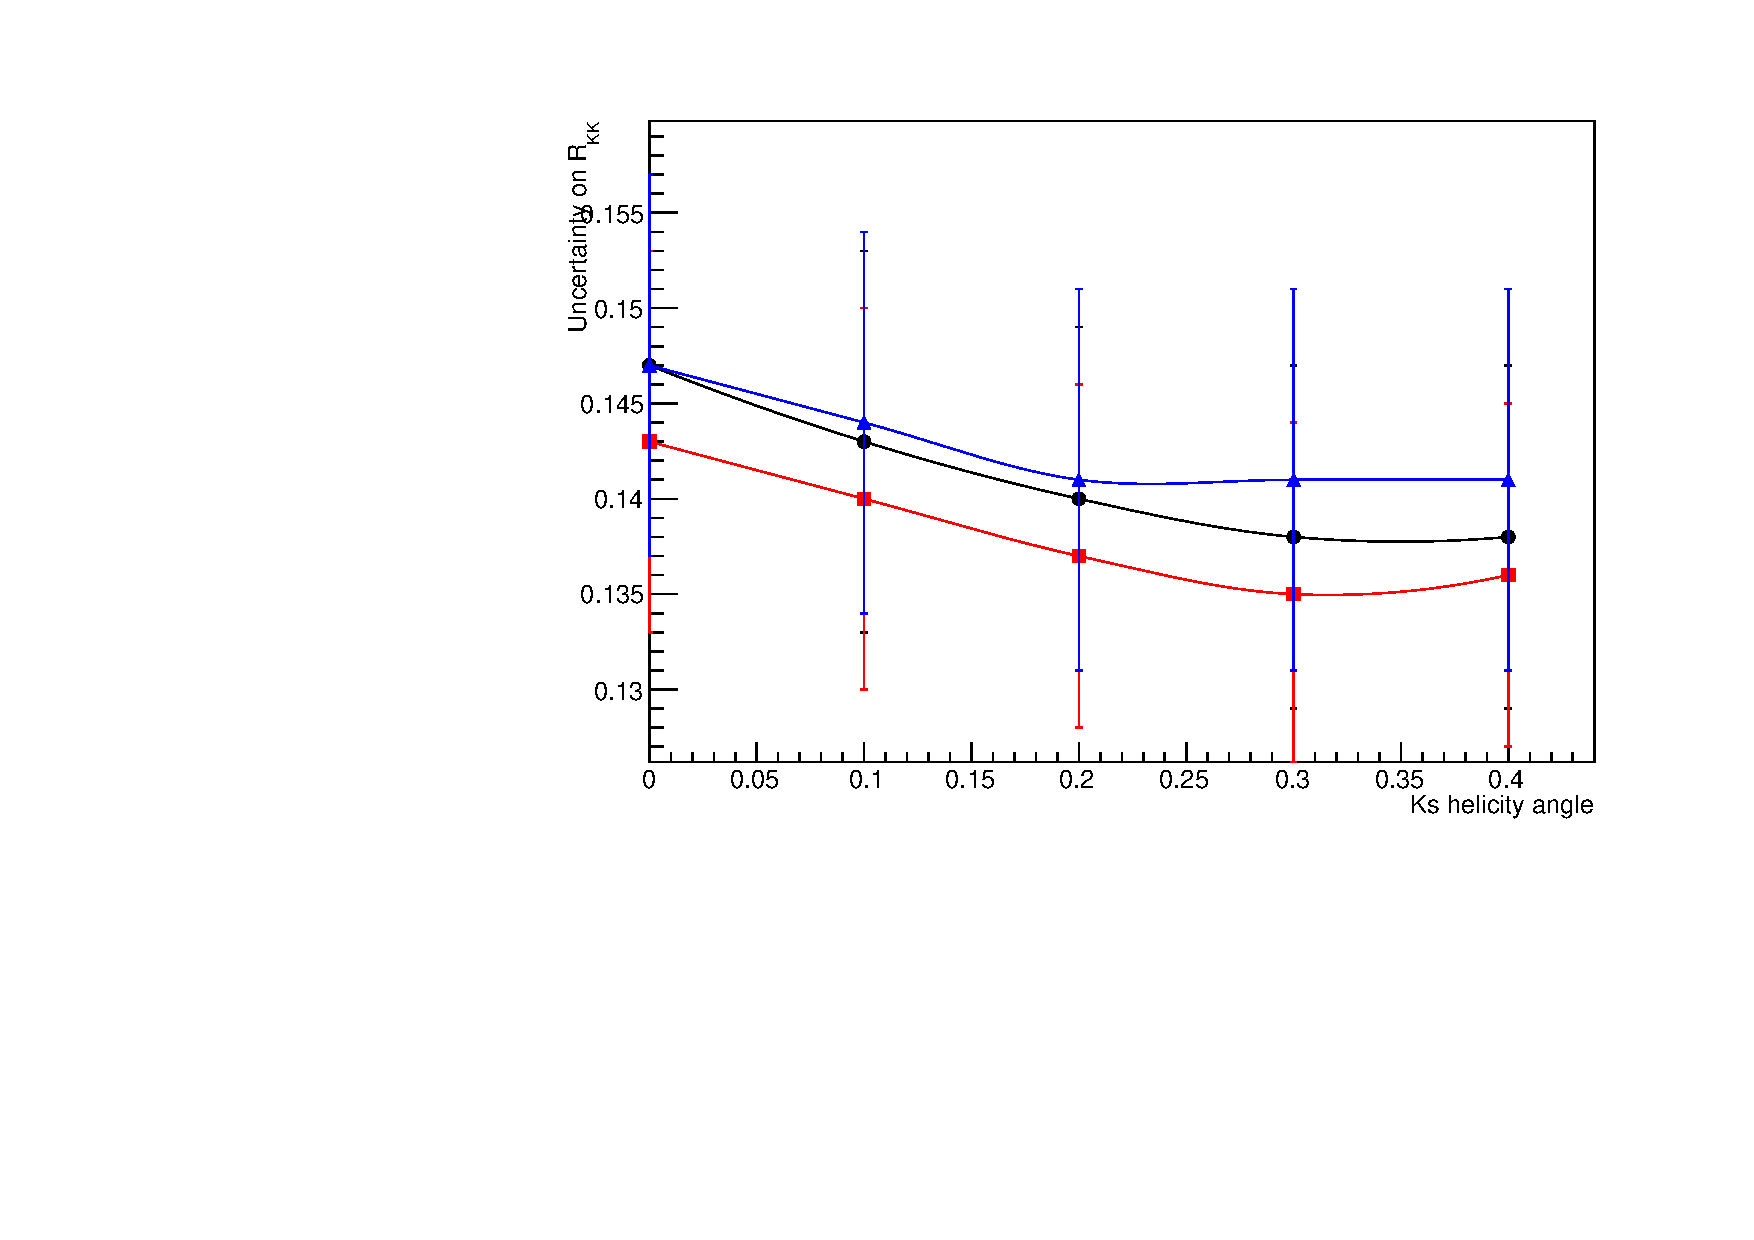
\includegraphics[width=0.8\linewidth]{figures/selection/optimisation.pdf}
\caption{Value of the uncertainty on \Rkk as a function of \KS helicity angle selection for different \Kstar mass selections. The reconstructed \Kstarm mass is required to lie within 50\mevcc (blue), 75\mevcc (red), or 100\mevcc (black) of the known \Kstar mass.}
\label{optimisation}
\end{figure}

\begin{figure}
\centering
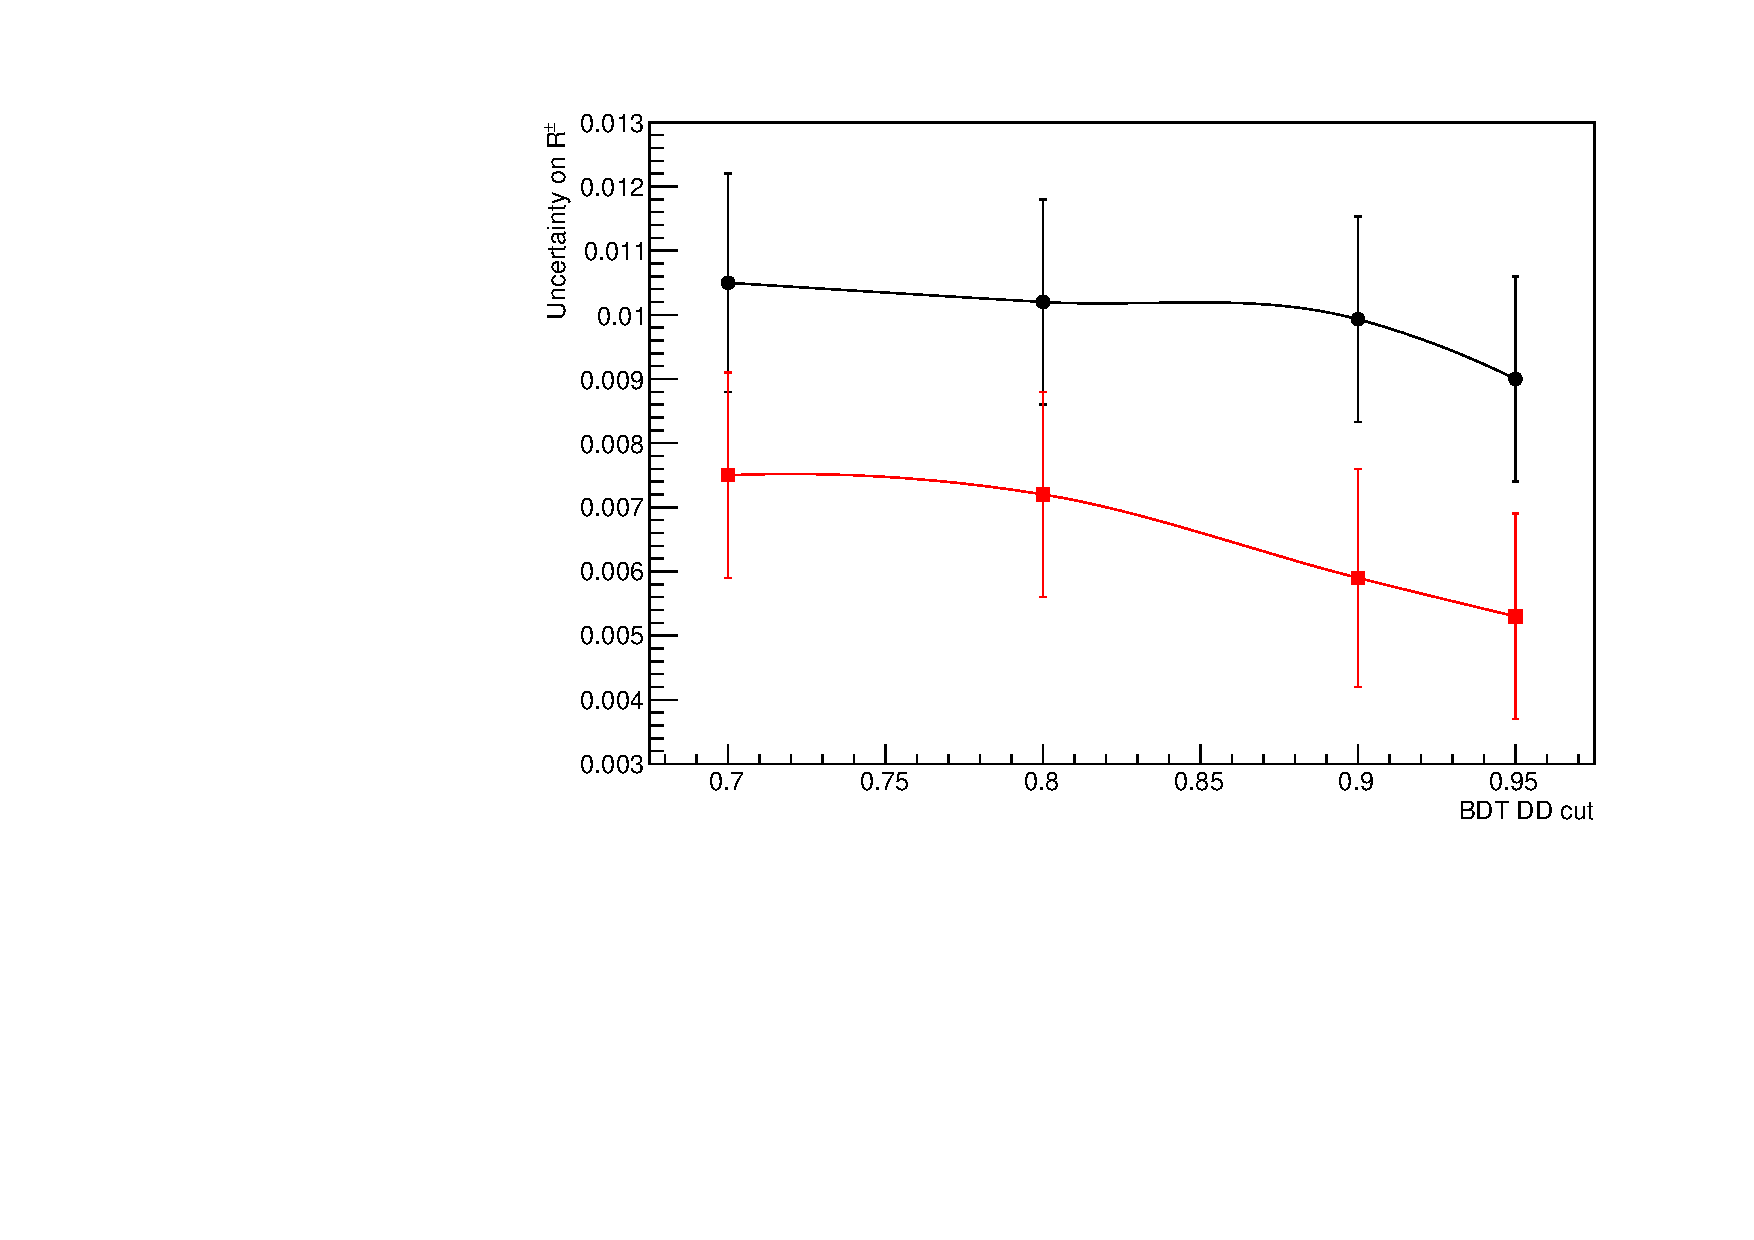
\includegraphics[width=0.8\linewidth]{figures/selection/ADSoptimisation.pdf}
\caption{Value of the uncertainty on \Rptwo (black) and \Rmtwo (red) as a function of BDT\_DD cut in the ADS mode. These pseudoexperiments are run with a BDT\_LL cut of 0.6 on all modes and BDT\_DD cut of 0.7 on all modes other than the ADS.}
\label{adsoptimisation}
\end{figure}

The pseudoexperiments described in this section are originally generated with an equal combinatorial rate in each of the \Dz decay modes. However, a significantly lower combinatorial rate is observed in data in the ADS modes compared to the corresponding favoured \kpi and \kpipipi modes. Consequently, changes in the combinatorial rate corresponding to differences observed in data are investigated. The choice of BDT selection for the ADS modes is found to remain optimal when tested against a scenario of the observed low combinatorial in the ADS mode. 

\subsection{Fitter bias in \CP fit}
\label{sec:cpfit:fitterbias}

In order to test the validity of the \CP fit model, data samples are generated for each of the bins according to the model described in Section \ref{sec:massfit}, and then by performing the \CP fit on the generated data, any biases, incorrect determination of the uncertainties, or instability in the \CP fit procedure can be observed. 

Pseudoexperiments are performed using the same procedure described in Section \ref{sec:cpfit:optimisation}, however in this case they are performed based on the final selection only using physics parameters $r_B = 0.1$, $\delta_B = 111^{\circ}$ and $\gamma = 70^{\circ}$. The results of the fit are found to have little sensitivity to the chosen value of $\delta_B$. As for the optimisation, the \CP fit is performed 1000 times, where each time the value of each the \CP observables and their associated uncertainty is extracted. The validity of the fit is tested by observing the pull distribution of each fit parameter $x$, which is given by,
\begin{equation*}
P_x = \begin{cases}
	\frac{x_{fit} - x_{gen}}{\sigma_x^-}, & \text{if $x_{fit} - x_{gen} >$ 0}. \\
	\frac{x_{gen} - x_{fit}}{\sigma_x^+}, & \text{if $x_{fit} - x_{gen} <$ 0}.
	\end{cases}
\end{equation*}
where $x_{fit}$ is the value of the parameter returned by the fit, $x_{gen}$ is the generated value of the parameter, and $\sigma_x^+$ and $\sigma_x^-$ are the upper and lower asymmetric uncertainties respectively. These asymmetric uncertainties are determined as described in Section \ref{sec:massfit:likelihood}. The pull distributions for each of the \CP observables are shown in Figure \ref{pulls}, where for each of the pull distributions a Gaussian fit is performed. All of these fitted Gaussians are all consistent with a mean of zero and width of one, which shows that the setup of the \CP fit is unbiased and the uncertainties are correctly determined. Additionally, all of the fits converge, therefore the fit is stable. 
 
%\begin{figure}[!h]
%\centering
%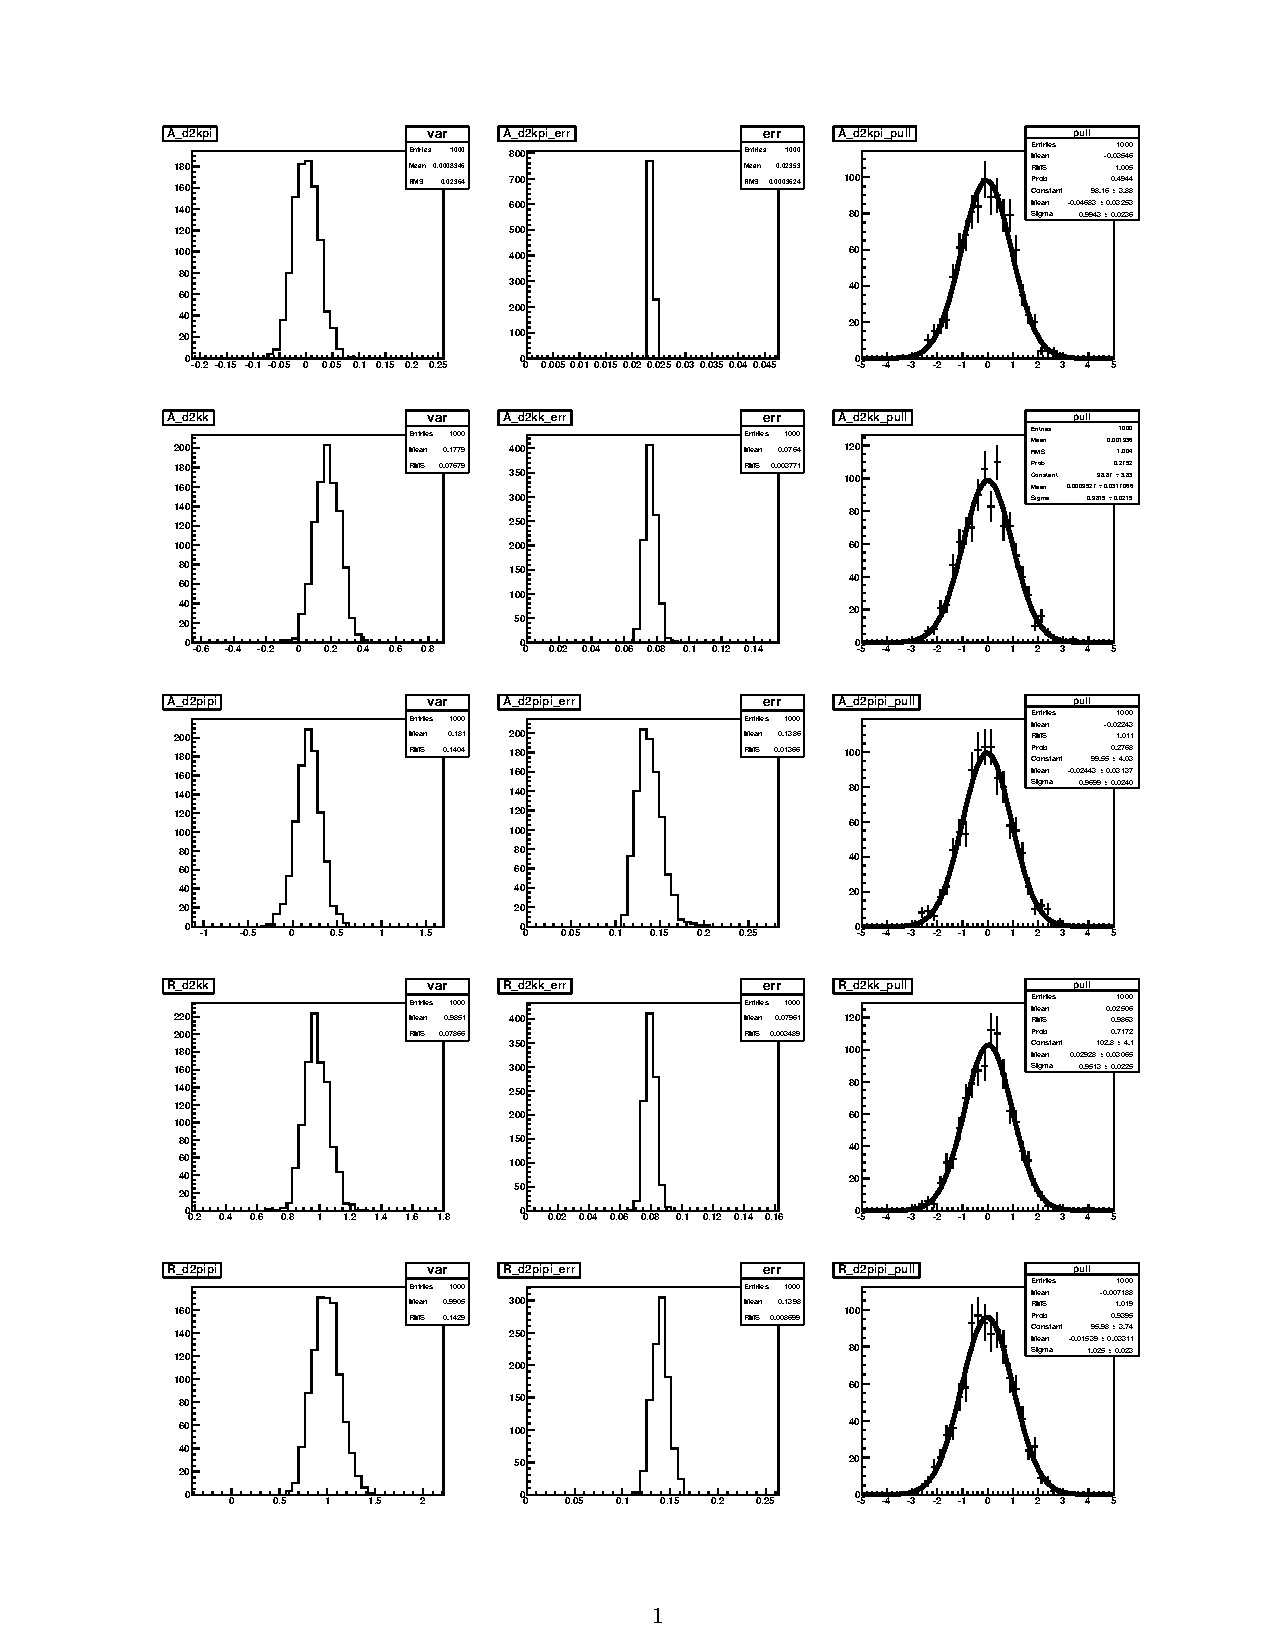
\includegraphics[page=1,trim = 0mm 24mm 0mm 15mm,clip,width=0.85\linewidth]{figures/results/toys.pdf}
%\includegraphics[page=2,trim = 0mm 165mm 0mm 15mm,clip,width=0.85\linewidth]{figures/results/toys.pdf}
%\caption{Results from pseudoexperiments for the two-body \CP observables in the fit. The left-hand column shows the fitted parameter distribution, the middle column shows the fit error distribution and the right-hand column are the pull distributions fitted with a Gaussian.}
%\label{pulls1}
%\end{figure}
%
%\begin{figure}[!h]
%\centering
%\includegraphics[page=2,trim = 0mm 24mm 0mm 113mm,clip,width=0.85\linewidth]{figures/results/toys.pdf}
%\includegraphics[page=3,trim = 0mm 165mm 0mm 15mm,clip,width=0.85\linewidth]{figures/results/toys.pdf}
%\caption{Results from pseudoexperiments for the four-body \CP observables in the fit. The left-hand column shows the fitted parameter distribution, the middle column shows the fit error distribution and the right-hand column are the pull distributions fitted with a Gaussian.}
%\label{pulls2}
%\end{figure}

\begin{figure}
\centering
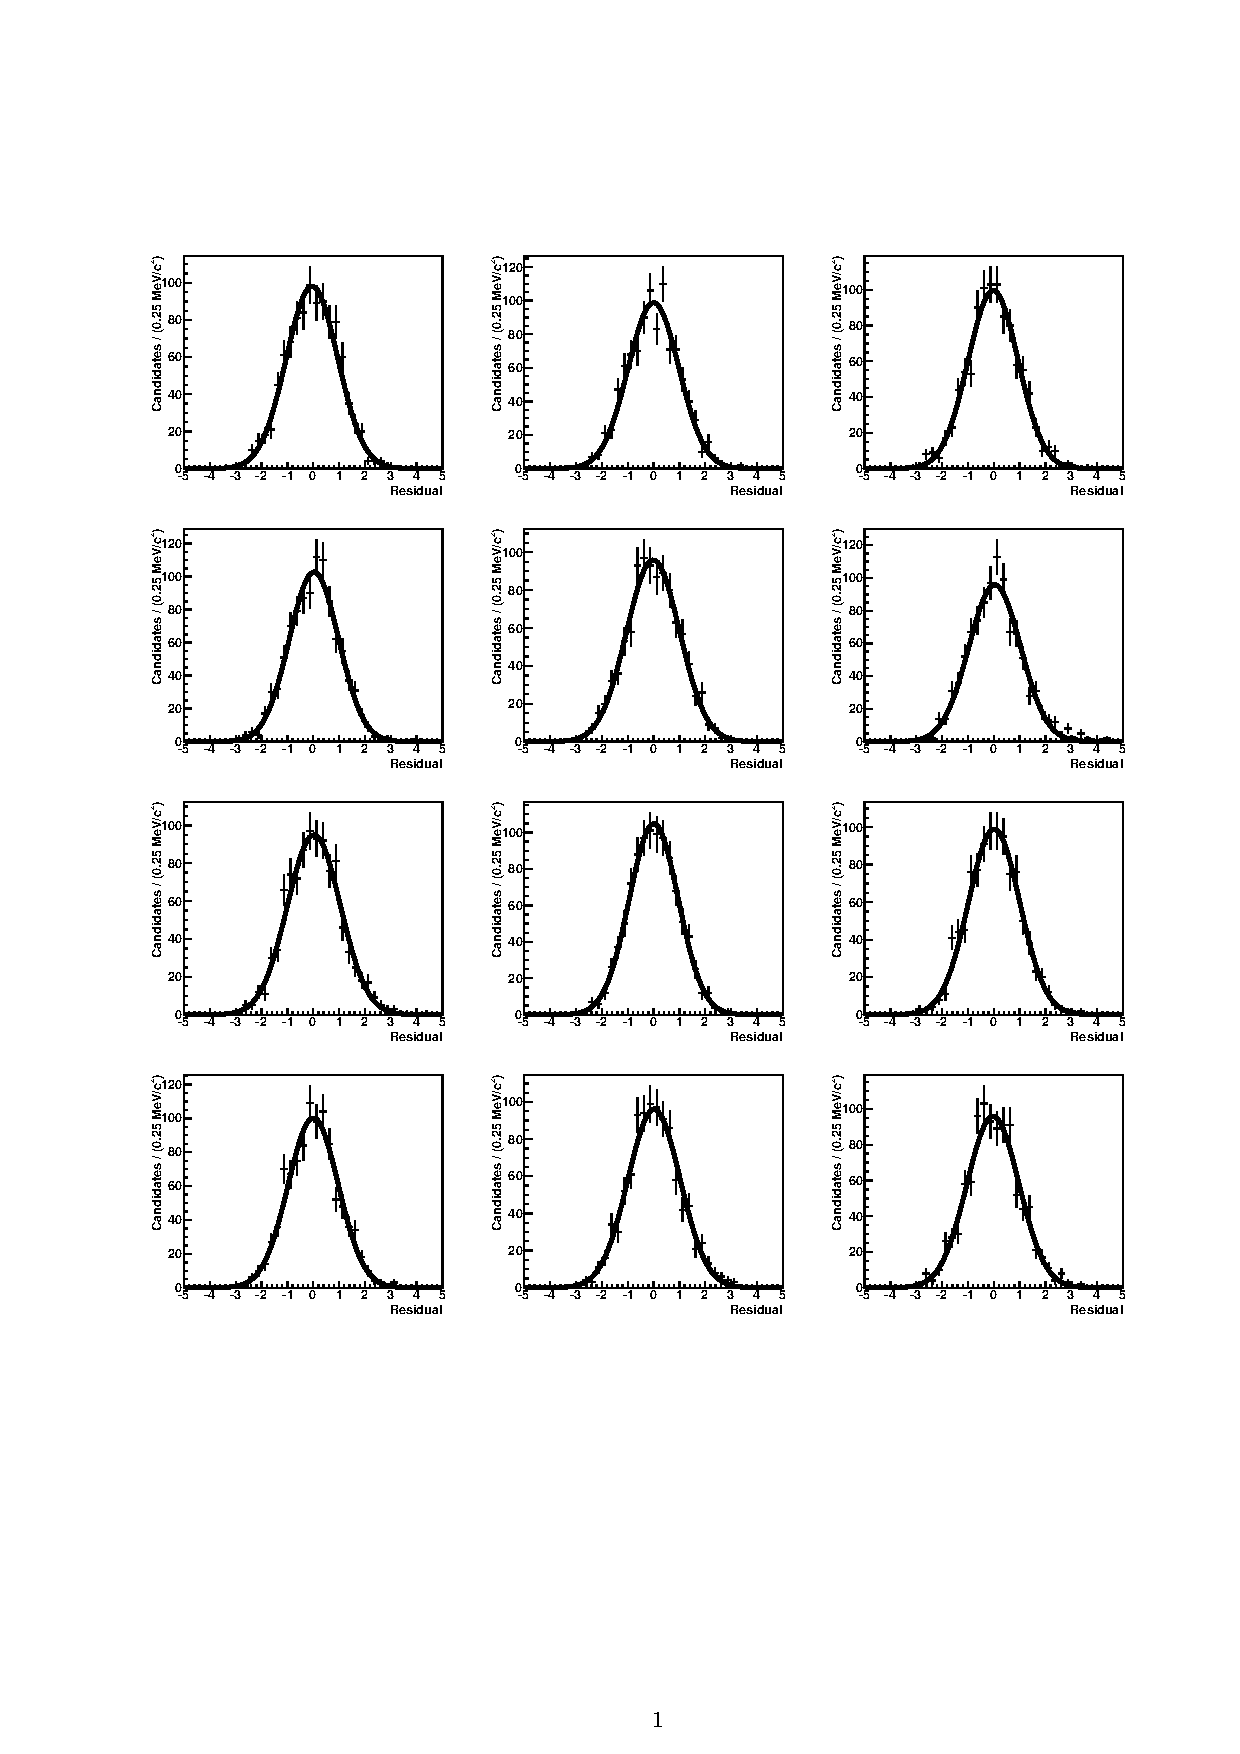
\includegraphics[trim = 18mm 70mm 18mm 30mm,clip,width=\linewidth]{figures/results/normaltoys.pdf}
\put(-380,420) {\Akpi}
\put(-240,420) {\Akk}
\put(-100,420) {\Apipi}
\put(-380,310) {\Rkk}
\put(-240,310) {\Rpipi}
\put(-100,310) {\Rmtwo}
\put(-380,200) {\Rptwo}
\put(-240,200) {\Akpipipi}
\put(-100,200) {\Apipipipi}
\put(-380,90) {\Rpipipipi}
\put(-240,90) {\Rmfour}
\put(-100,90) {\Rpfour}
\caption{Pull distributions, $P_x$, from pseudoexperiments for all of the \CP observables in the fit. The points represent the data and the curve is the fitted Gaussian.}
\label{pulls}
\end{figure}

%%%%%%%%%%%%%%%%%%%%%%%%
\section{Fit results}
\label{sec:cpfit:results}

The \CP fit described in Section \ref{sec:cpfit:setup} is performed on data, with mass projections shown in Figures \ref{results2body} and \ref{results4body}. The results look similar for different \KS reconstruction types and data types, however for illustrative purposes only one of these categories is shown, corresponding to Run 2 DD candidates. This bin is chosen as it contains the highest number of events. Figure \ref{results2body} shows a slight asymmetry in the \kk and \pipi modes, however, there is a much more obvious asymmetry observed in the \pik mode, which occurs in the opposite direction. In the \pik mode, the \Bp decay has a higher yield than the \Bm decay, whereas in the \kk and \pipi modes the \Bm decay has a higher yield than the \Bp decay. The four-body modes, shown in Figure \ref{results4body}, display the same characteristics, but with fewer events.

Table \ref{cpfitresultsphysics} shows the \CP fit results for the \CP observables of interest. There is no significant asymmetry observed in the GLW and quasi-GLW modes, i.e. \Akk, \Apipi and \Apipipipi are all consistent with zero. However, for the two-body ADS mode, \Rptwo is significantly larger than \Rmtwo, showing asymmetry in this mode. The four-body ADS mode shows a similar behaviour, however the asymmetry is less significant. It can also be seen that \Akpi and \Akpipipi are consistent with zero, as expected due to the very low level of interference in these modes. Additionally, \Akk and \Apipi are in agreement with each other and \Rkk and \Rpipi are in agreement with each other, which is consistent with expectation. These \CP observables are expected to have the same value corresponding to the observables $A_{CP+}$ and $R_{CP+}$ respectively, given in Equations \ref{exp_Acp} and \ref{exp_Rcp}.

Table \ref{cpfitresultsshapes} shows the fit results for the favoured \kpi and \kpipipi signal yields and the shape parameters. It can be seen that both the mean and the width of the signal peak in the two-body and four-body modes are consistent with each other. The yields are significantly higher in \runtwo compared to \runone even though the integrated luminosity in \runtwo is lower. In fact, the yield per unit of integrated luminosity is about 3 times higher in \runone compared to \runtwo, which is driven by the increase in centre-of-mass energy in \runtwo. 

All the combinatorial yields are left to vary in the \CP fit for each of the different bins, and they are found to be consistent between \Bm and \Bp, as expected. However, there is a significantly higher combinatorial yield in the \kpi mode than the \pik mode. This difference is also observed between the \kpipipi and \pikpipi modes, but to a lesser extent. This observed difference in background level is consistent with a significant fraction of the combinatorial background coming from \decay{\Bm}{\D\pim X} decays combined with a real but unrelated \KS meson. 

The fitted signal yields obtained from running the fit with \Bp and \Bm samples combined are given in Table \ref{fittedyields}. When comparing the ratio of the two-body signal yields with the favoured mode, with the ratio of the branching fractions of the different \Dz modes, it can be observed that the results are consistent with the branching fractions. Both the \kk mode and \pik mode showing a slight excess compared to the expected yield. For the four-body modes, the ratio of \kpipipi to \pipipipi signal yields is consistent with their relative branching fractions.

\begin{figure}
\newlength{\imageheight}
\settoheight{\imageheight}{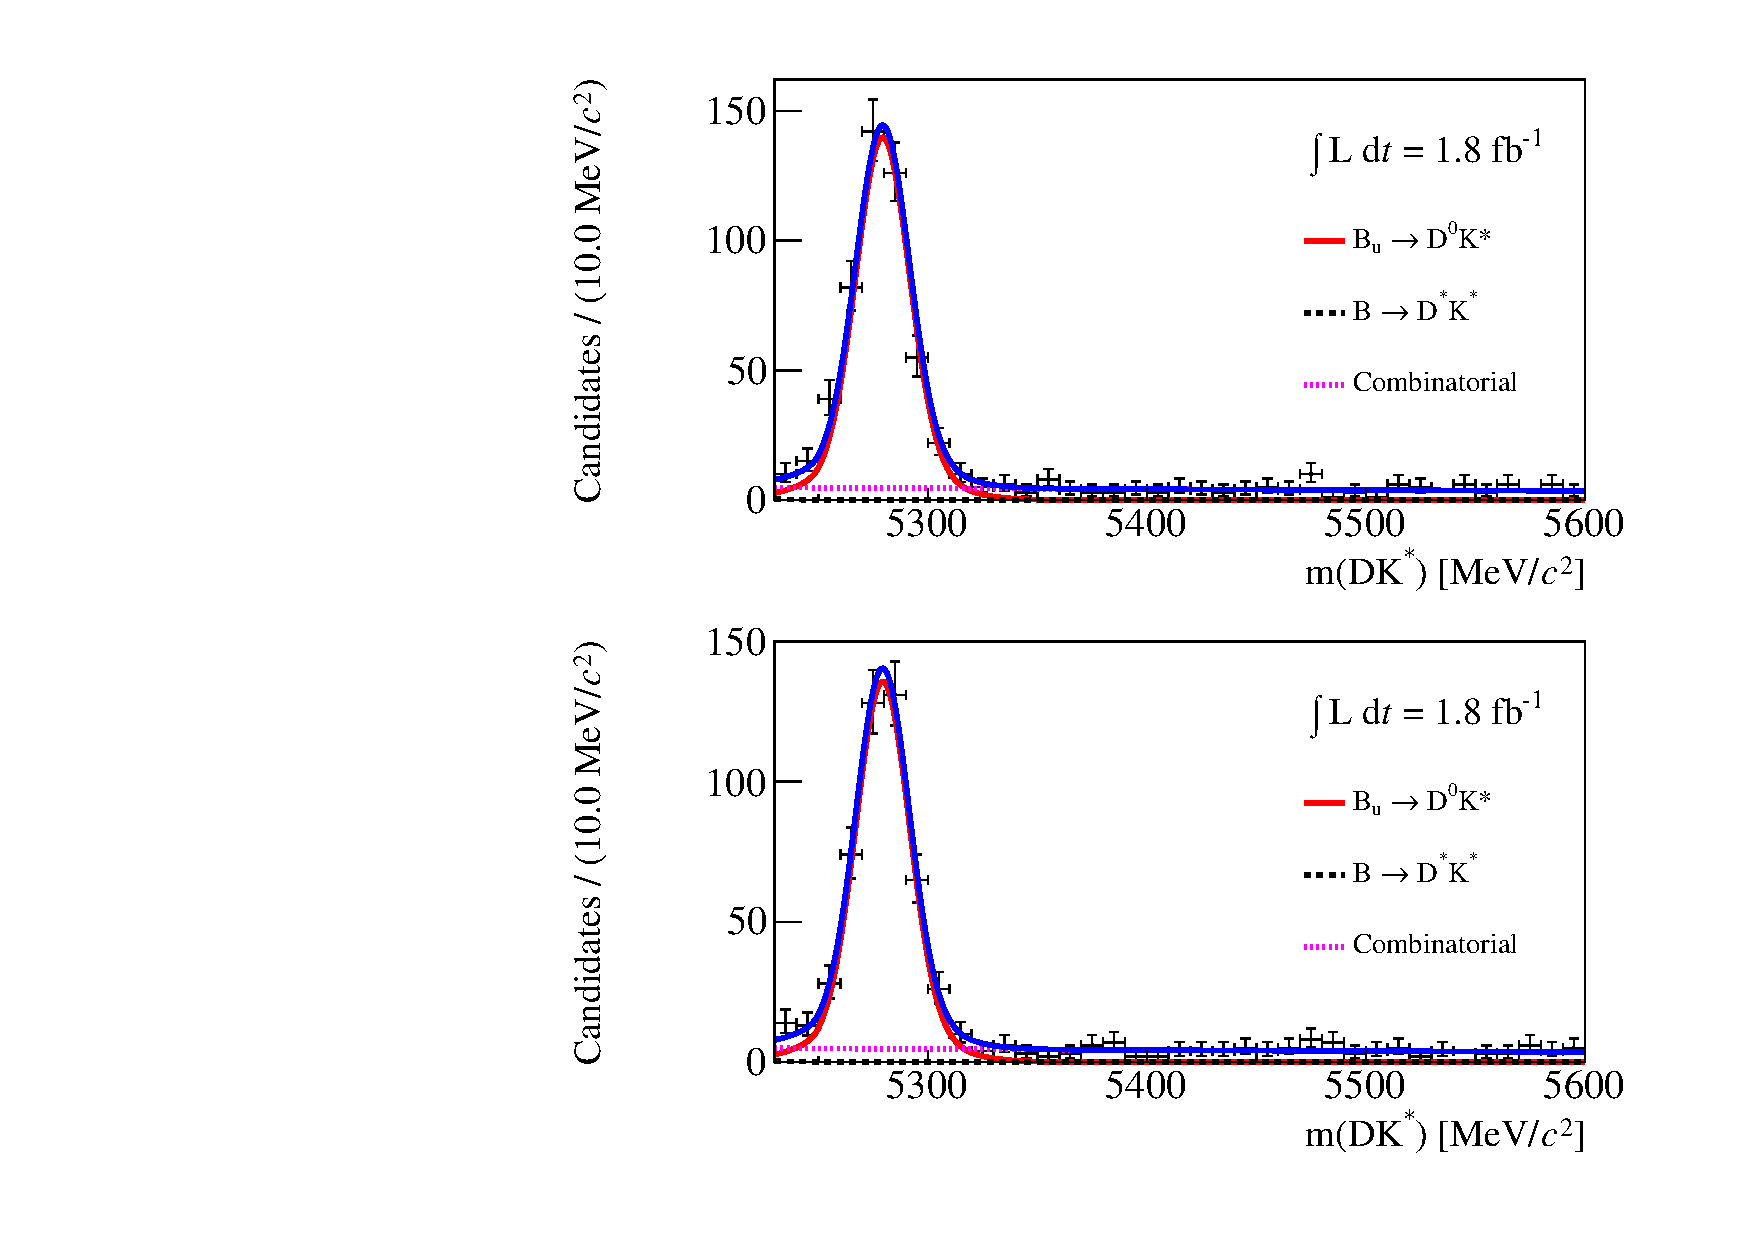
\includegraphics{figures/results/canvas_d2kpi_DD_run2.pdf}}
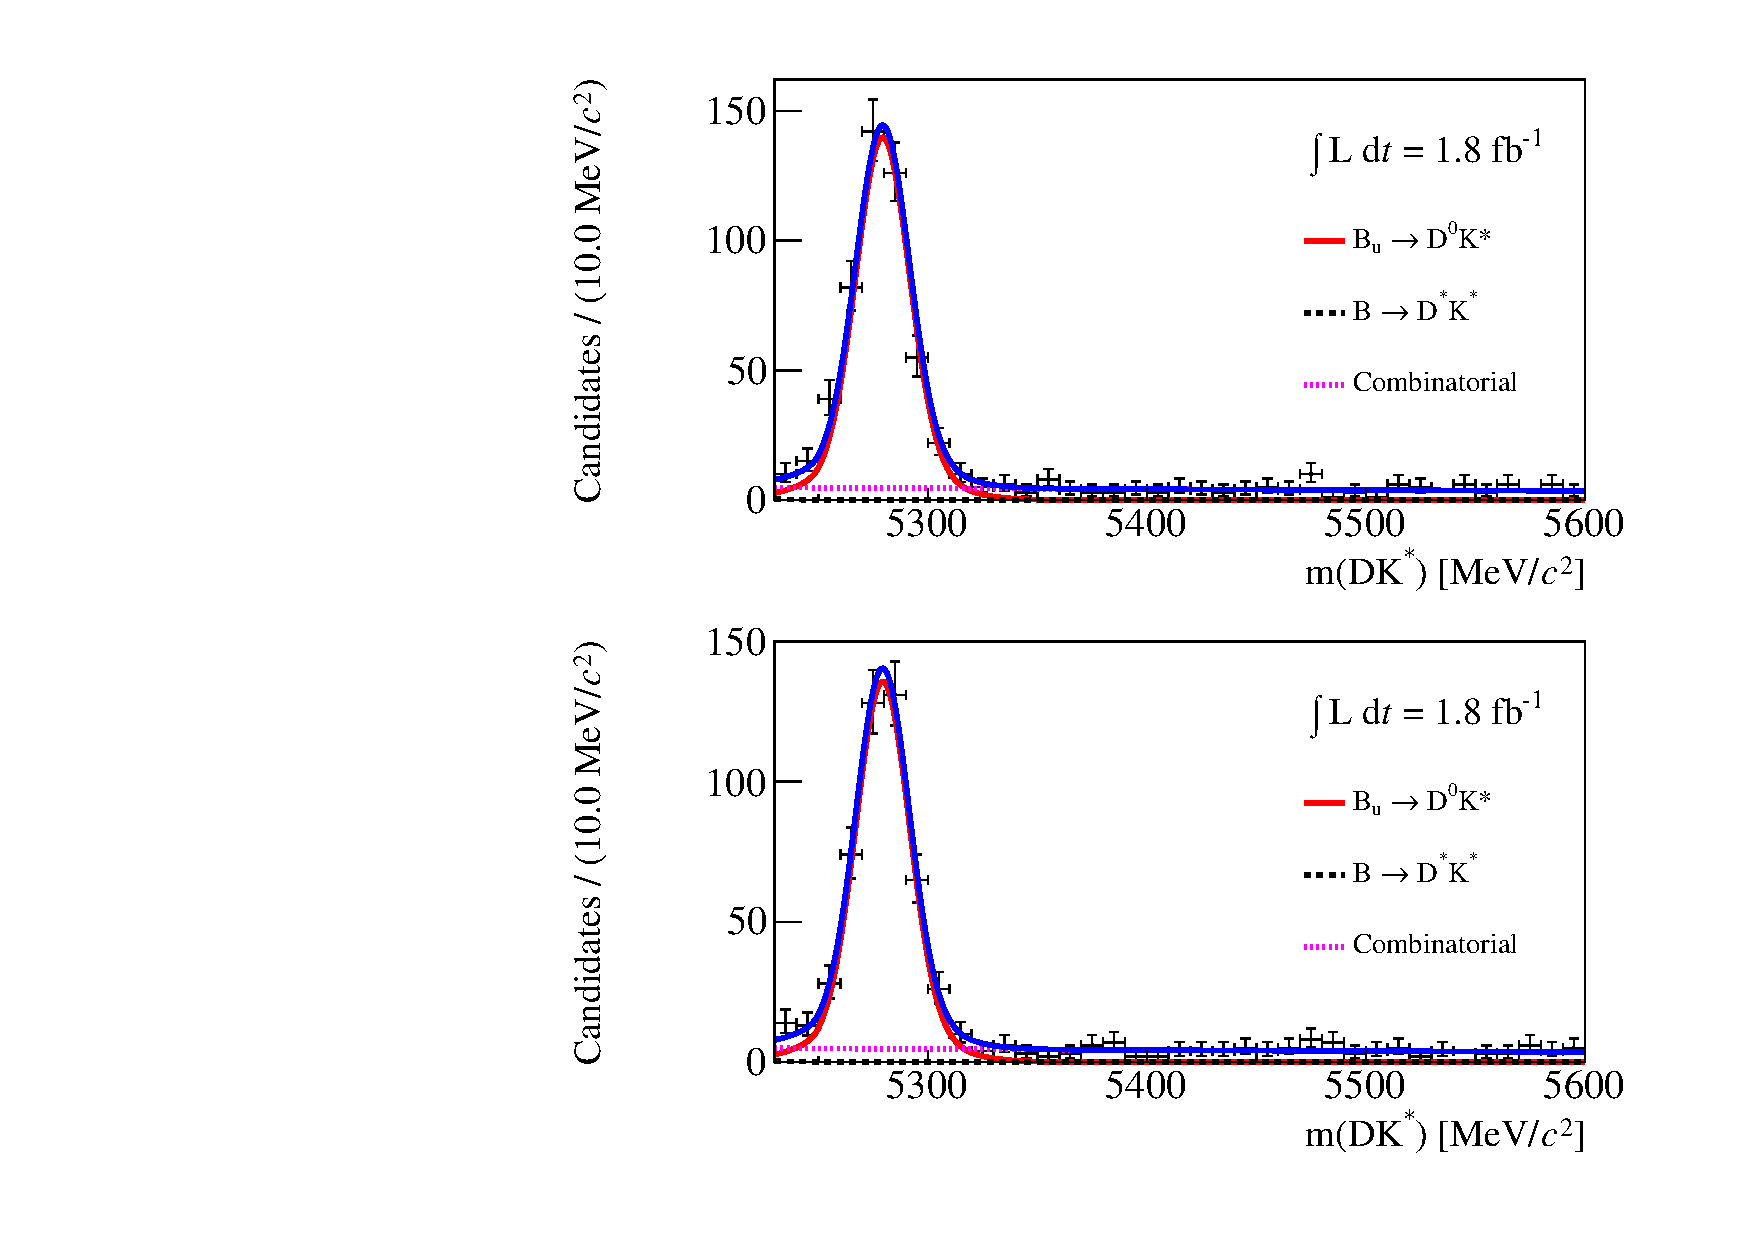
\includegraphics[trim = 0 0.5\imageheight{} 0 0,clip,width=0.5\linewidth]{figures/results/canvas_d2kpi_DD_run2.pdf}
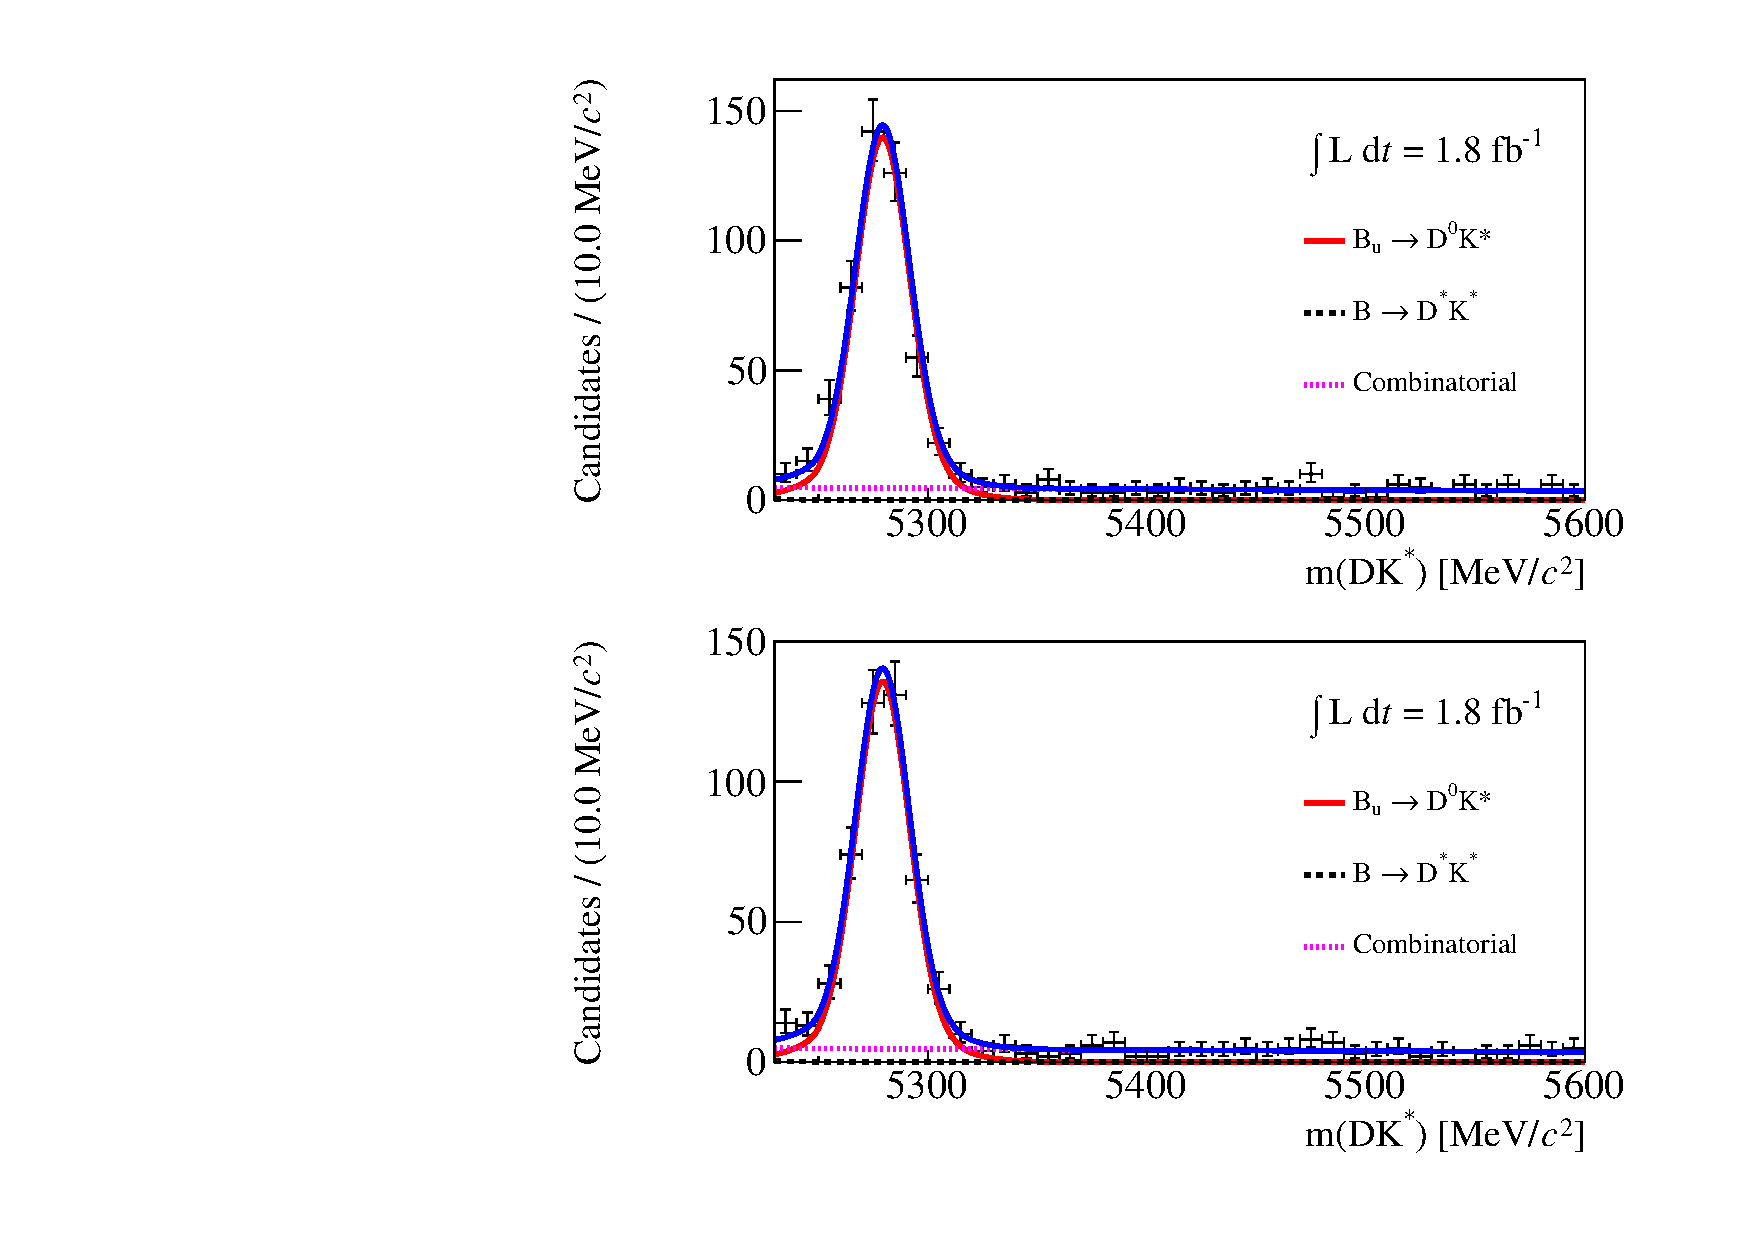
\includegraphics[trim = 0 0 0 0.5\imageheight{},clip,width=0.5\linewidth]{figures/results/canvas_d2kpi_DD_run2.pdf}
\hfill
\settoheight{\imageheight}{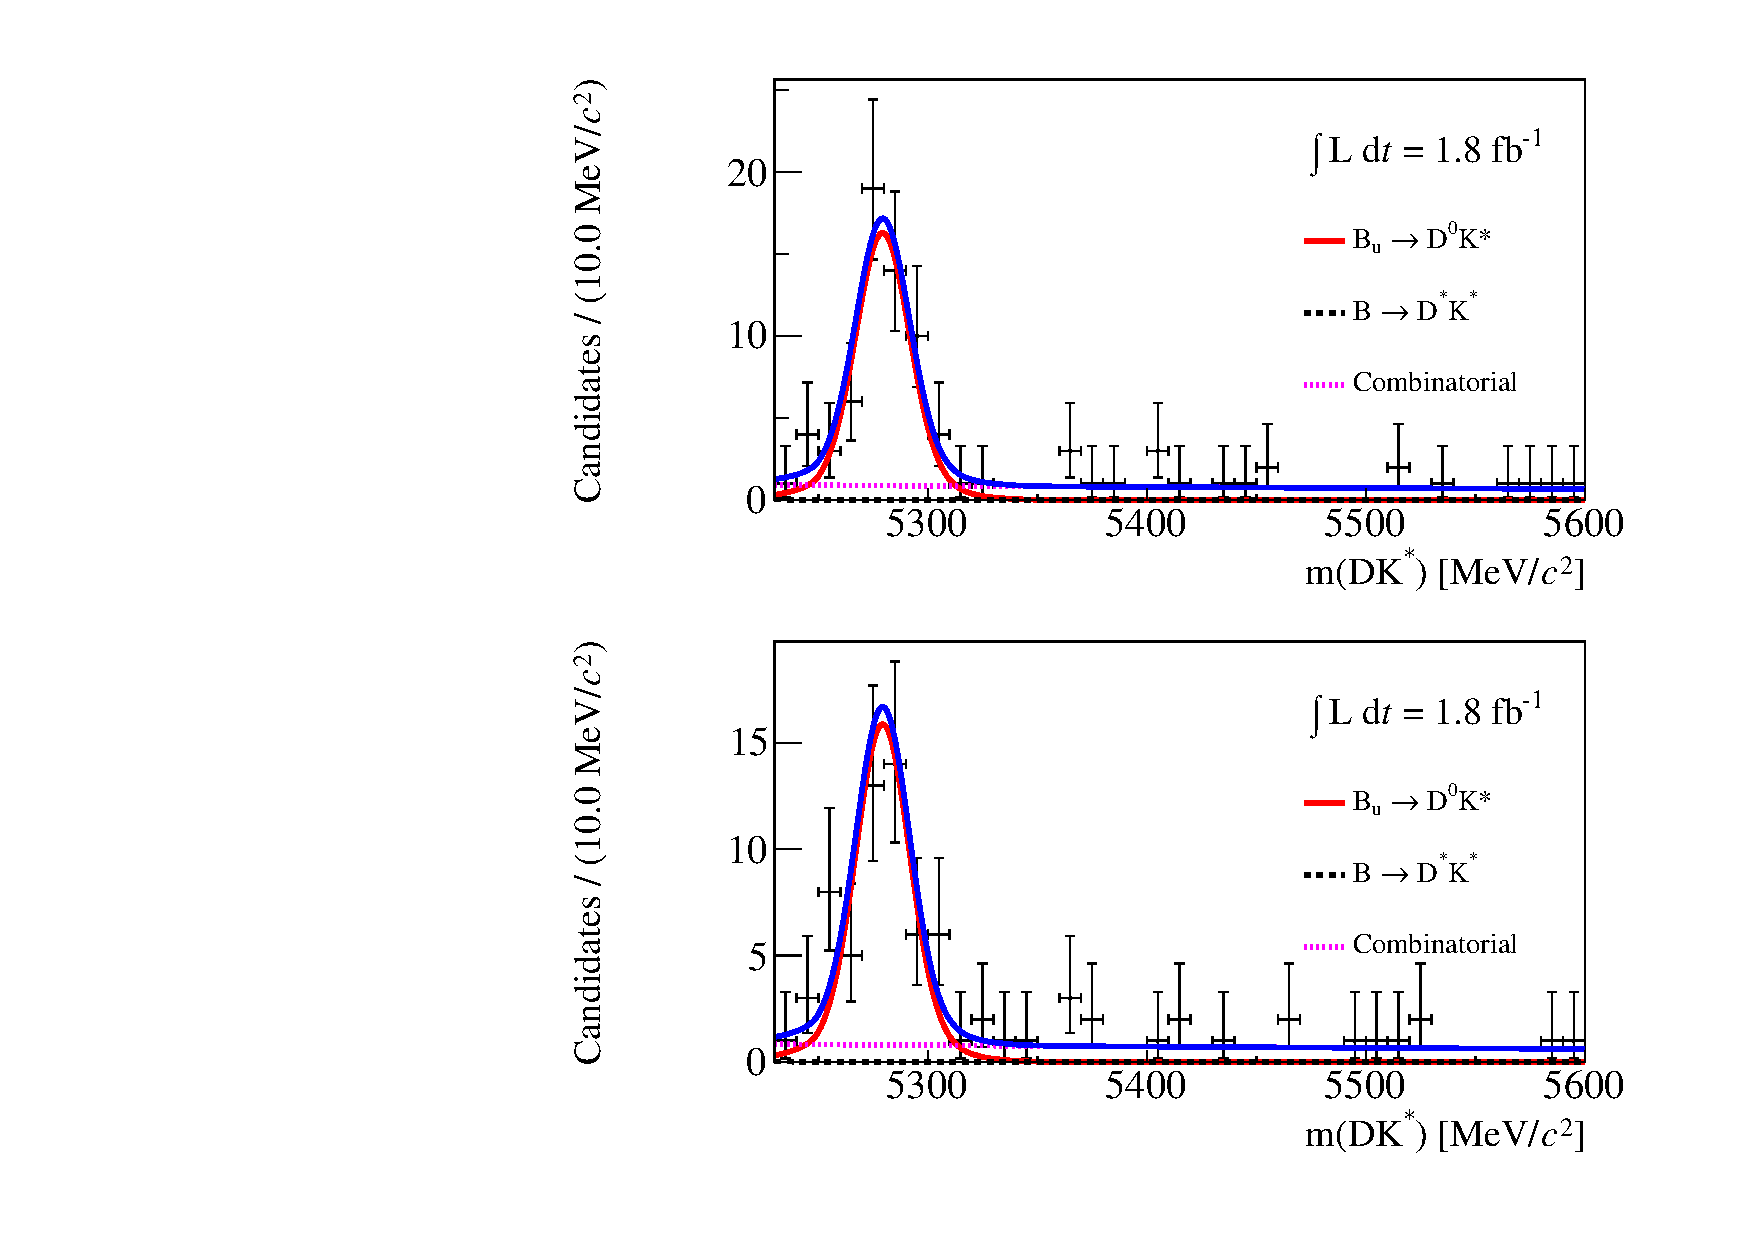
\includegraphics{figures/results/canvas_d2kk_DD_run2.pdf}}
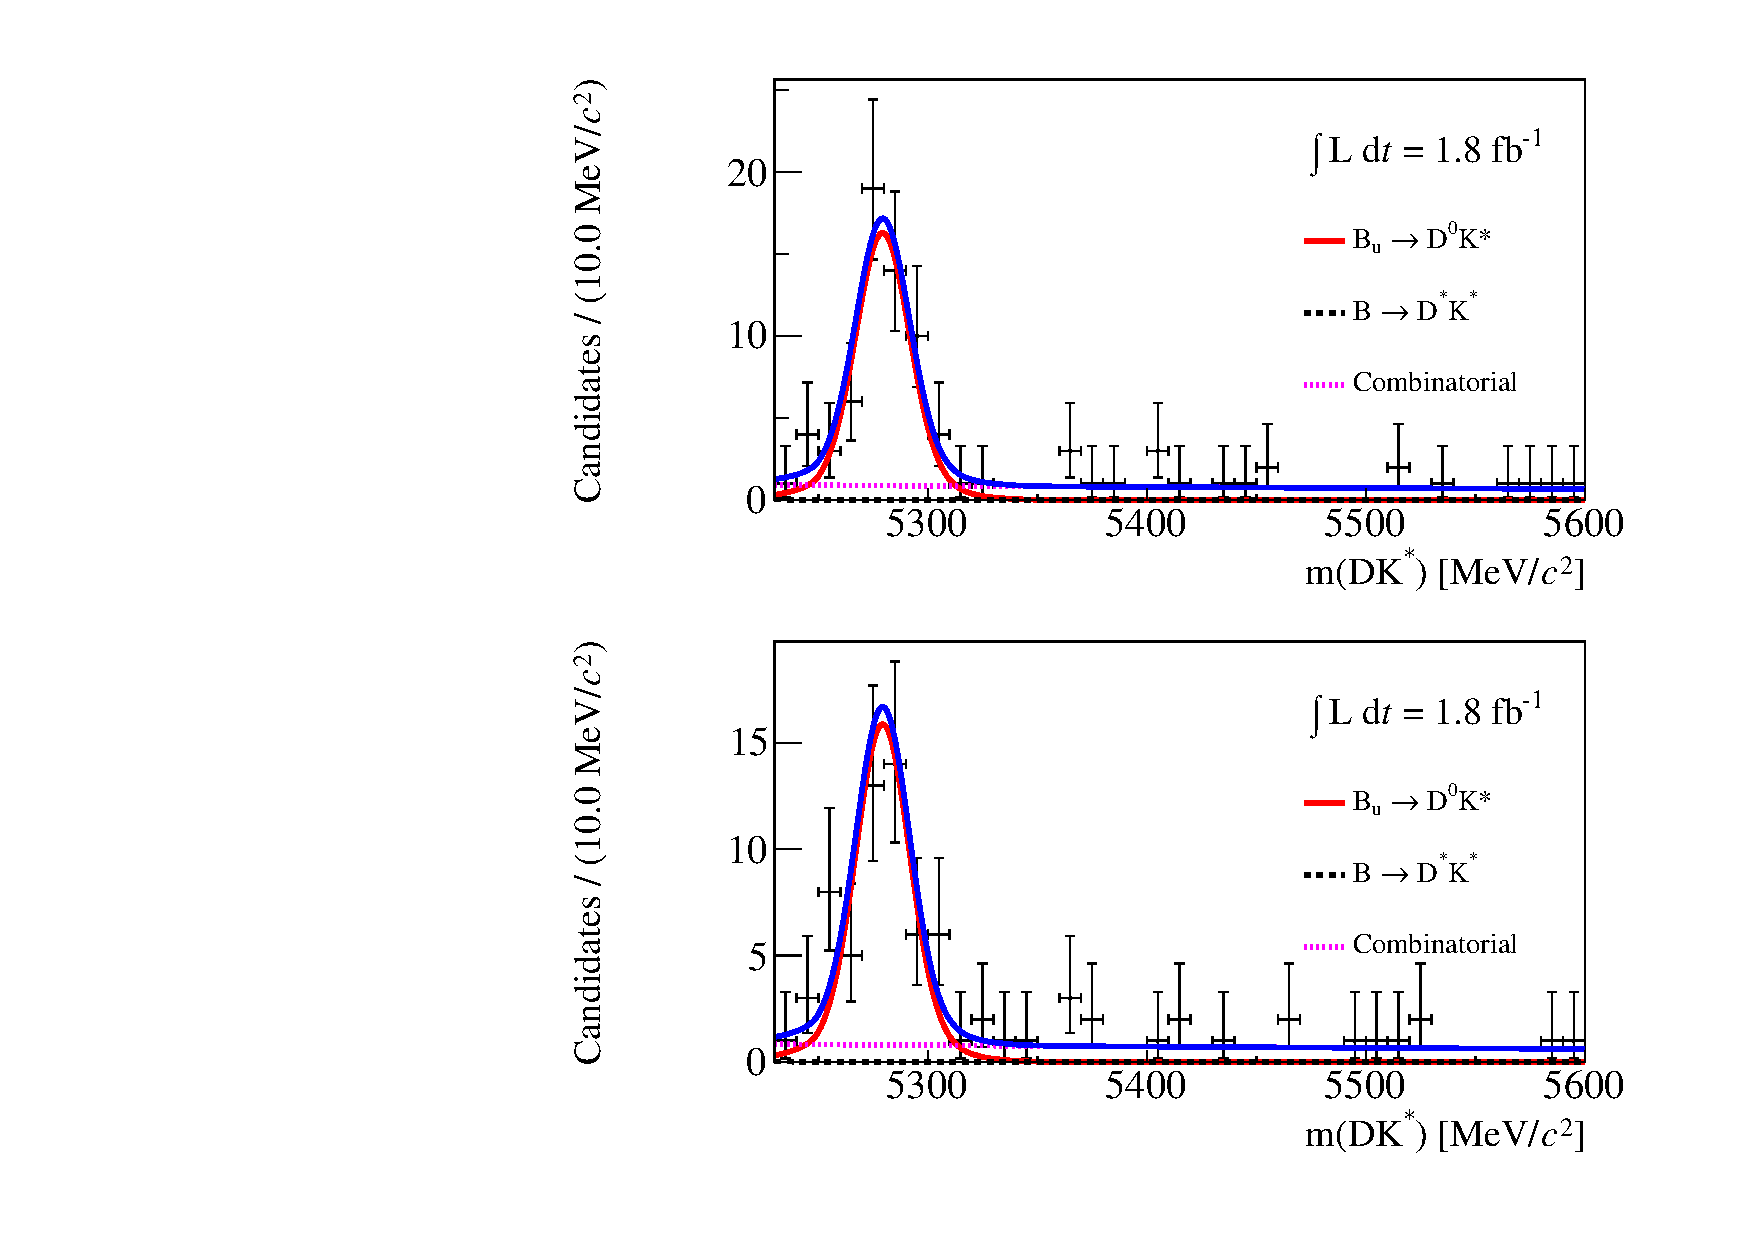
\includegraphics[trim = 0 0.5\imageheight{} 0 0,clip,width=0.5\linewidth]{figures/results/canvas_d2kk_DD_run2.pdf}
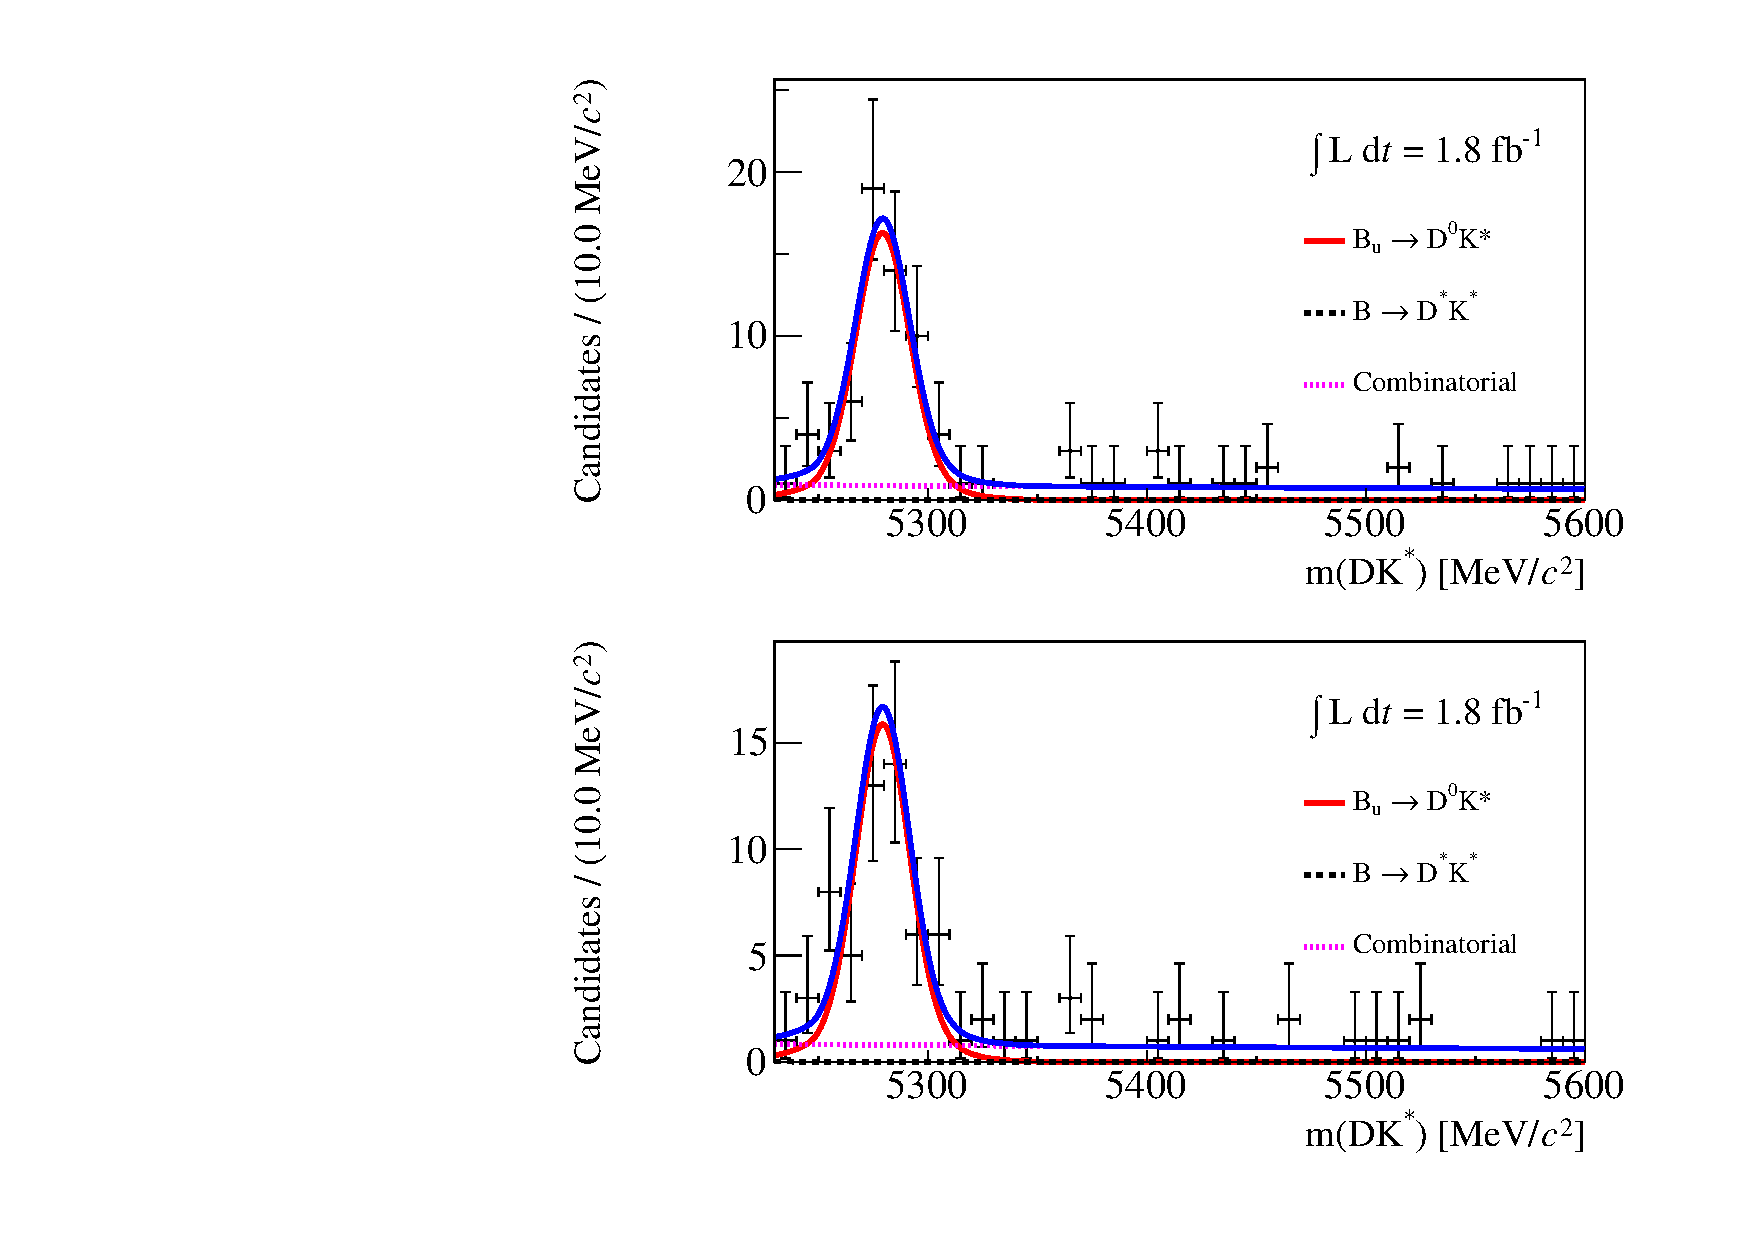
\includegraphics[trim = 0 0 0 0.5\imageheight{},clip,width=0.5\linewidth]{figures/results/canvas_d2kk_DD_run2.pdf}
\hfill
\settoheight{\imageheight}{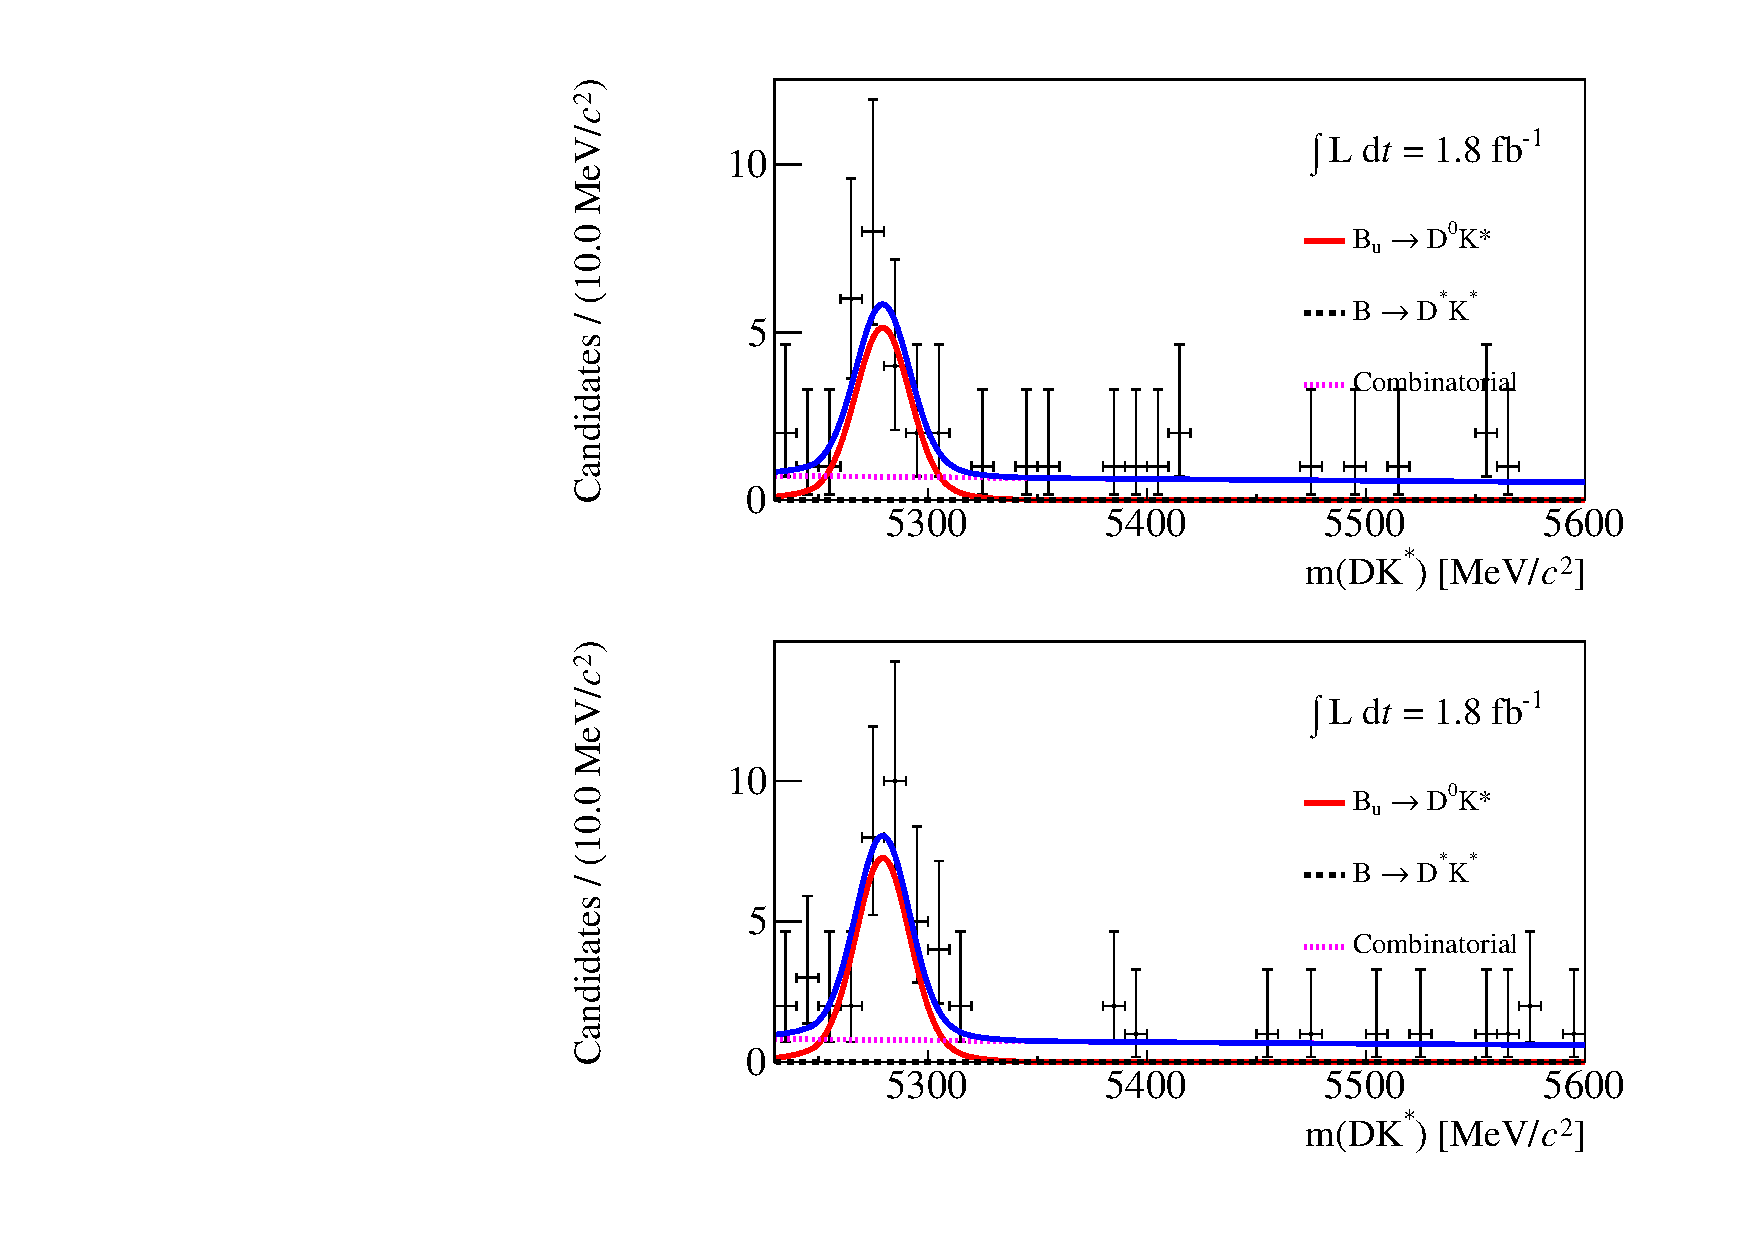
\includegraphics{figures/results/canvas_d2pipi_DD_run2.pdf}}
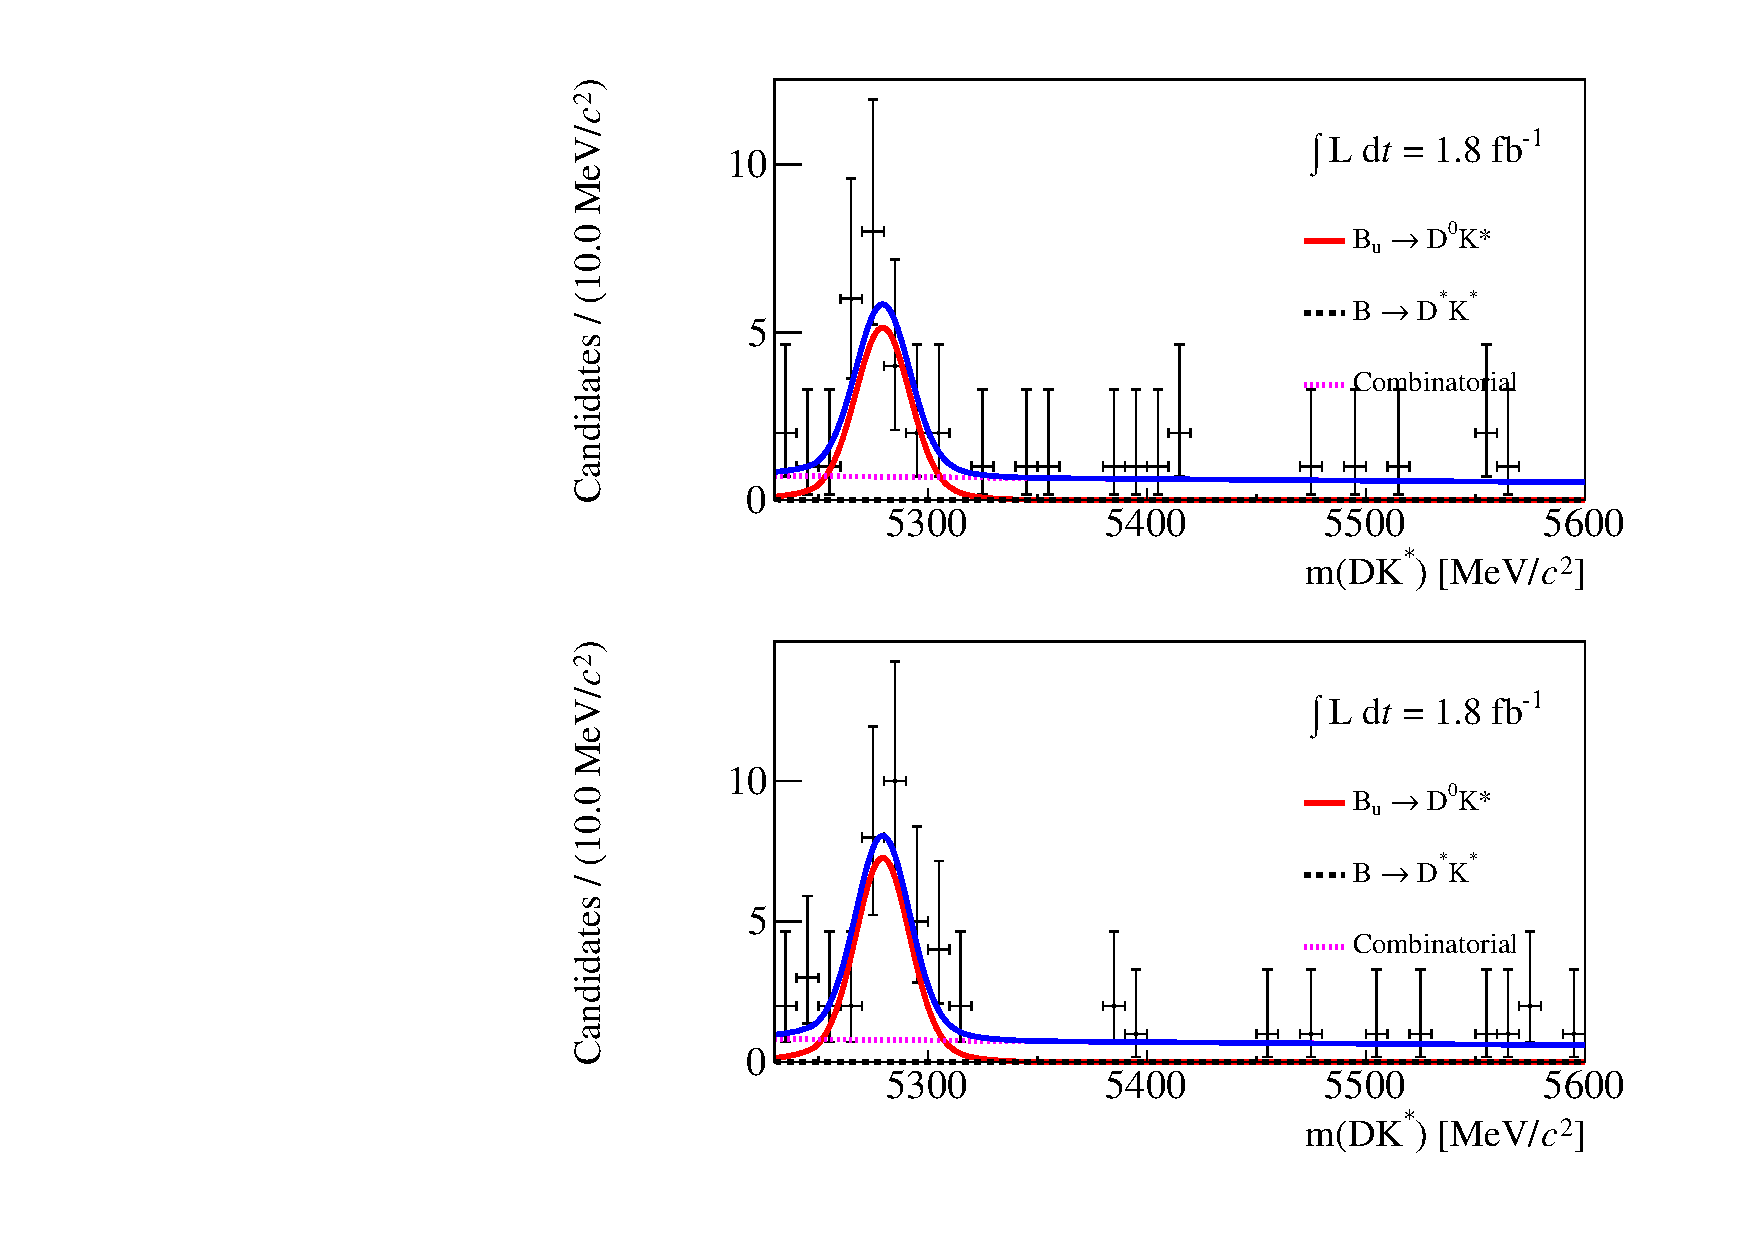
\includegraphics[trim = 0 0.5\imageheight{} 0 0,clip,width=0.5\linewidth]{figures/results/canvas_d2pipi_DD_run2.pdf}
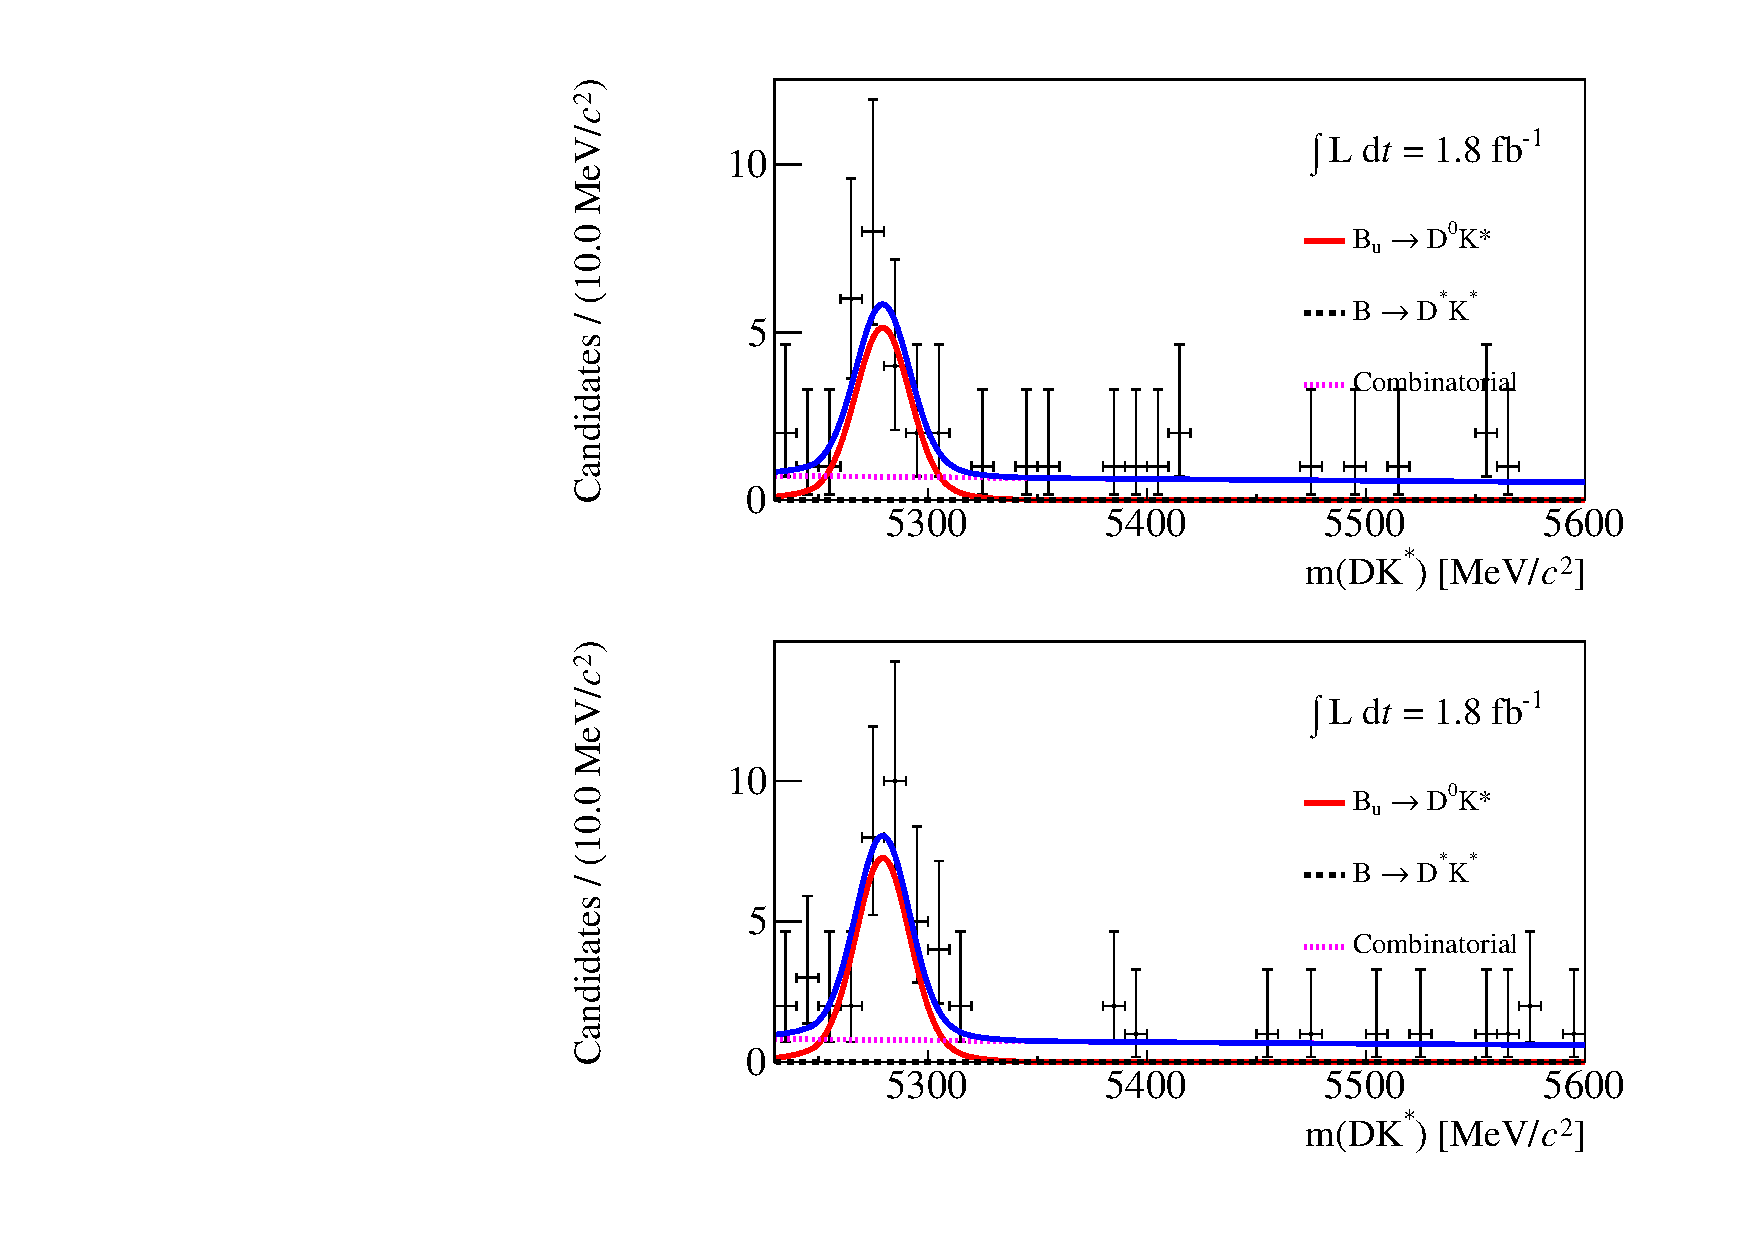
\includegraphics[trim = 0 0 0 0.5\imageheight{},clip,width=0.5\linewidth]{figures/results/canvas_d2pipi_DD_run2.pdf}
\hfill
\settoheight{\imageheight}{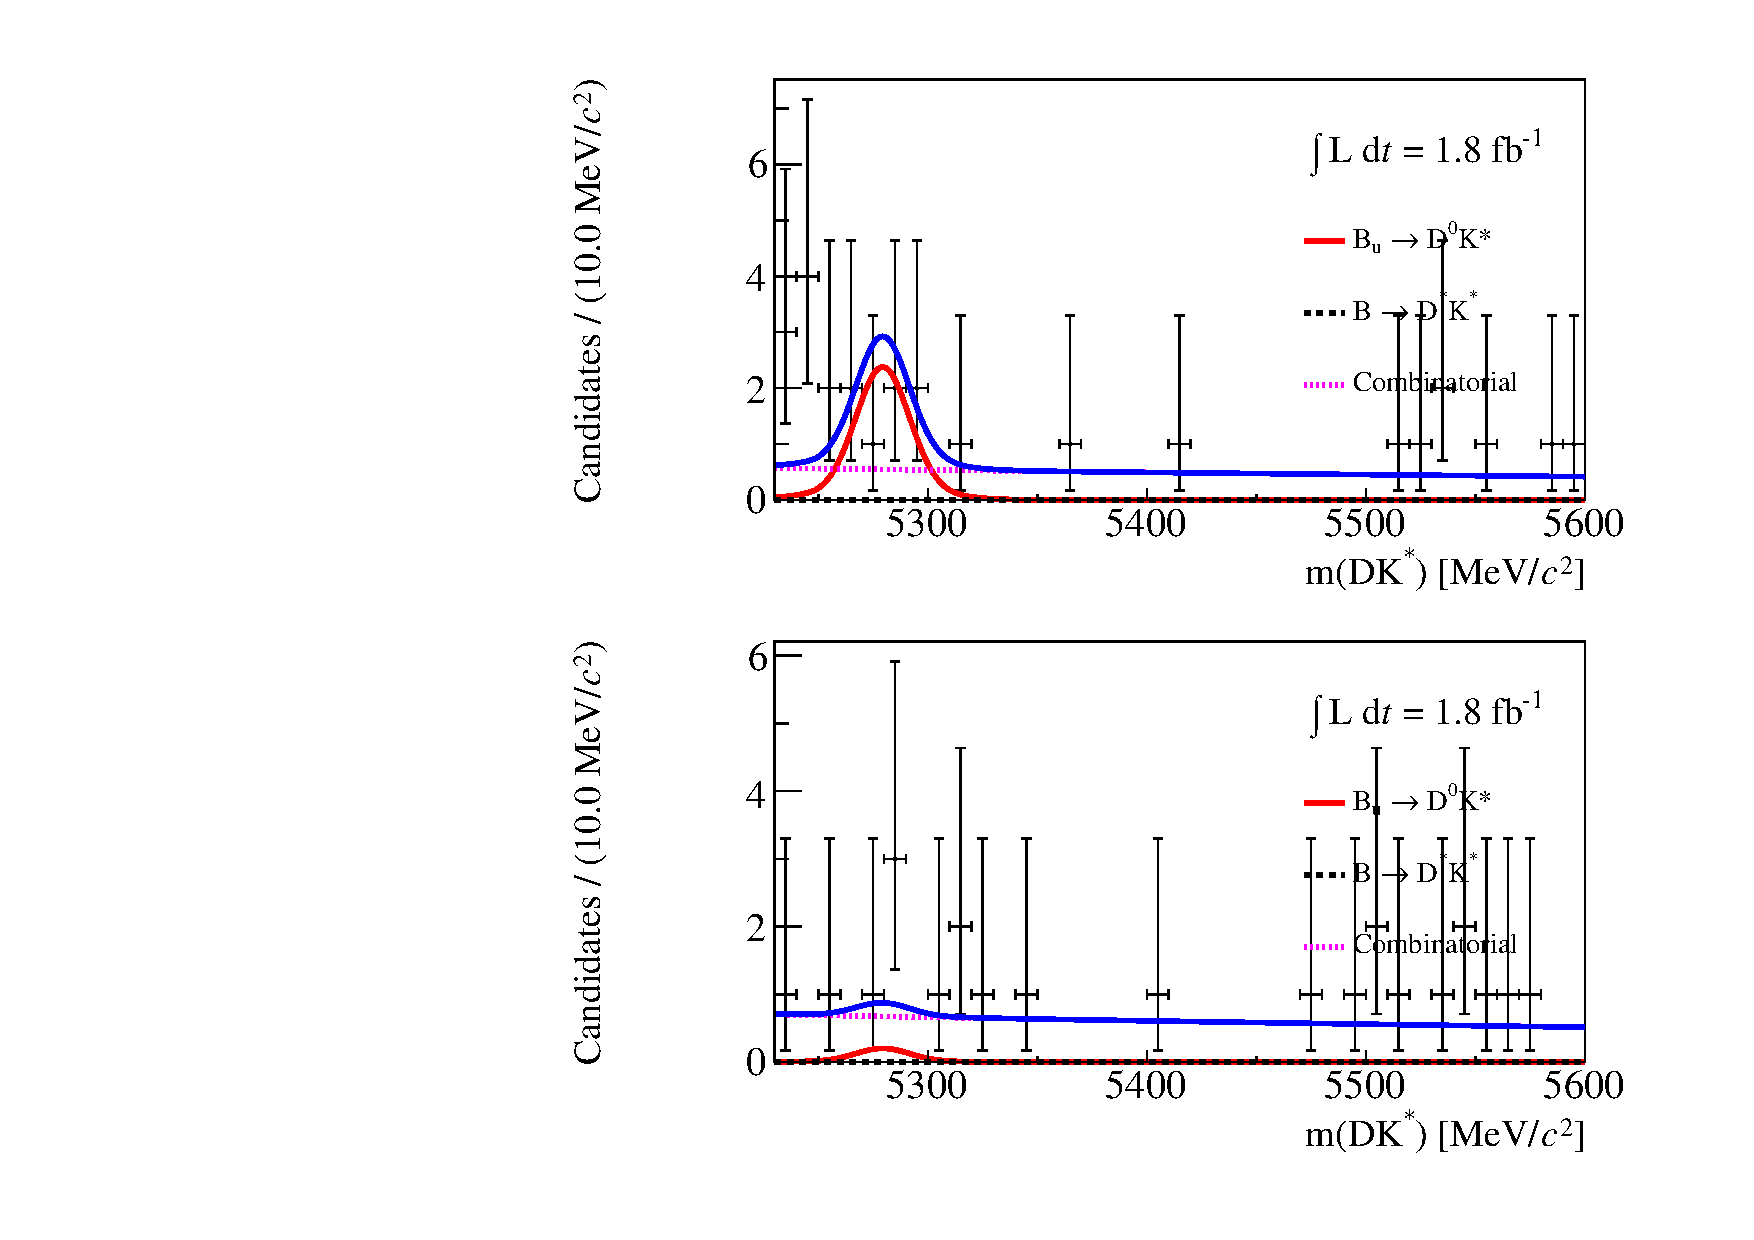
\includegraphics{figures/results/canvas_d2pik_DD_run2.pdf}}
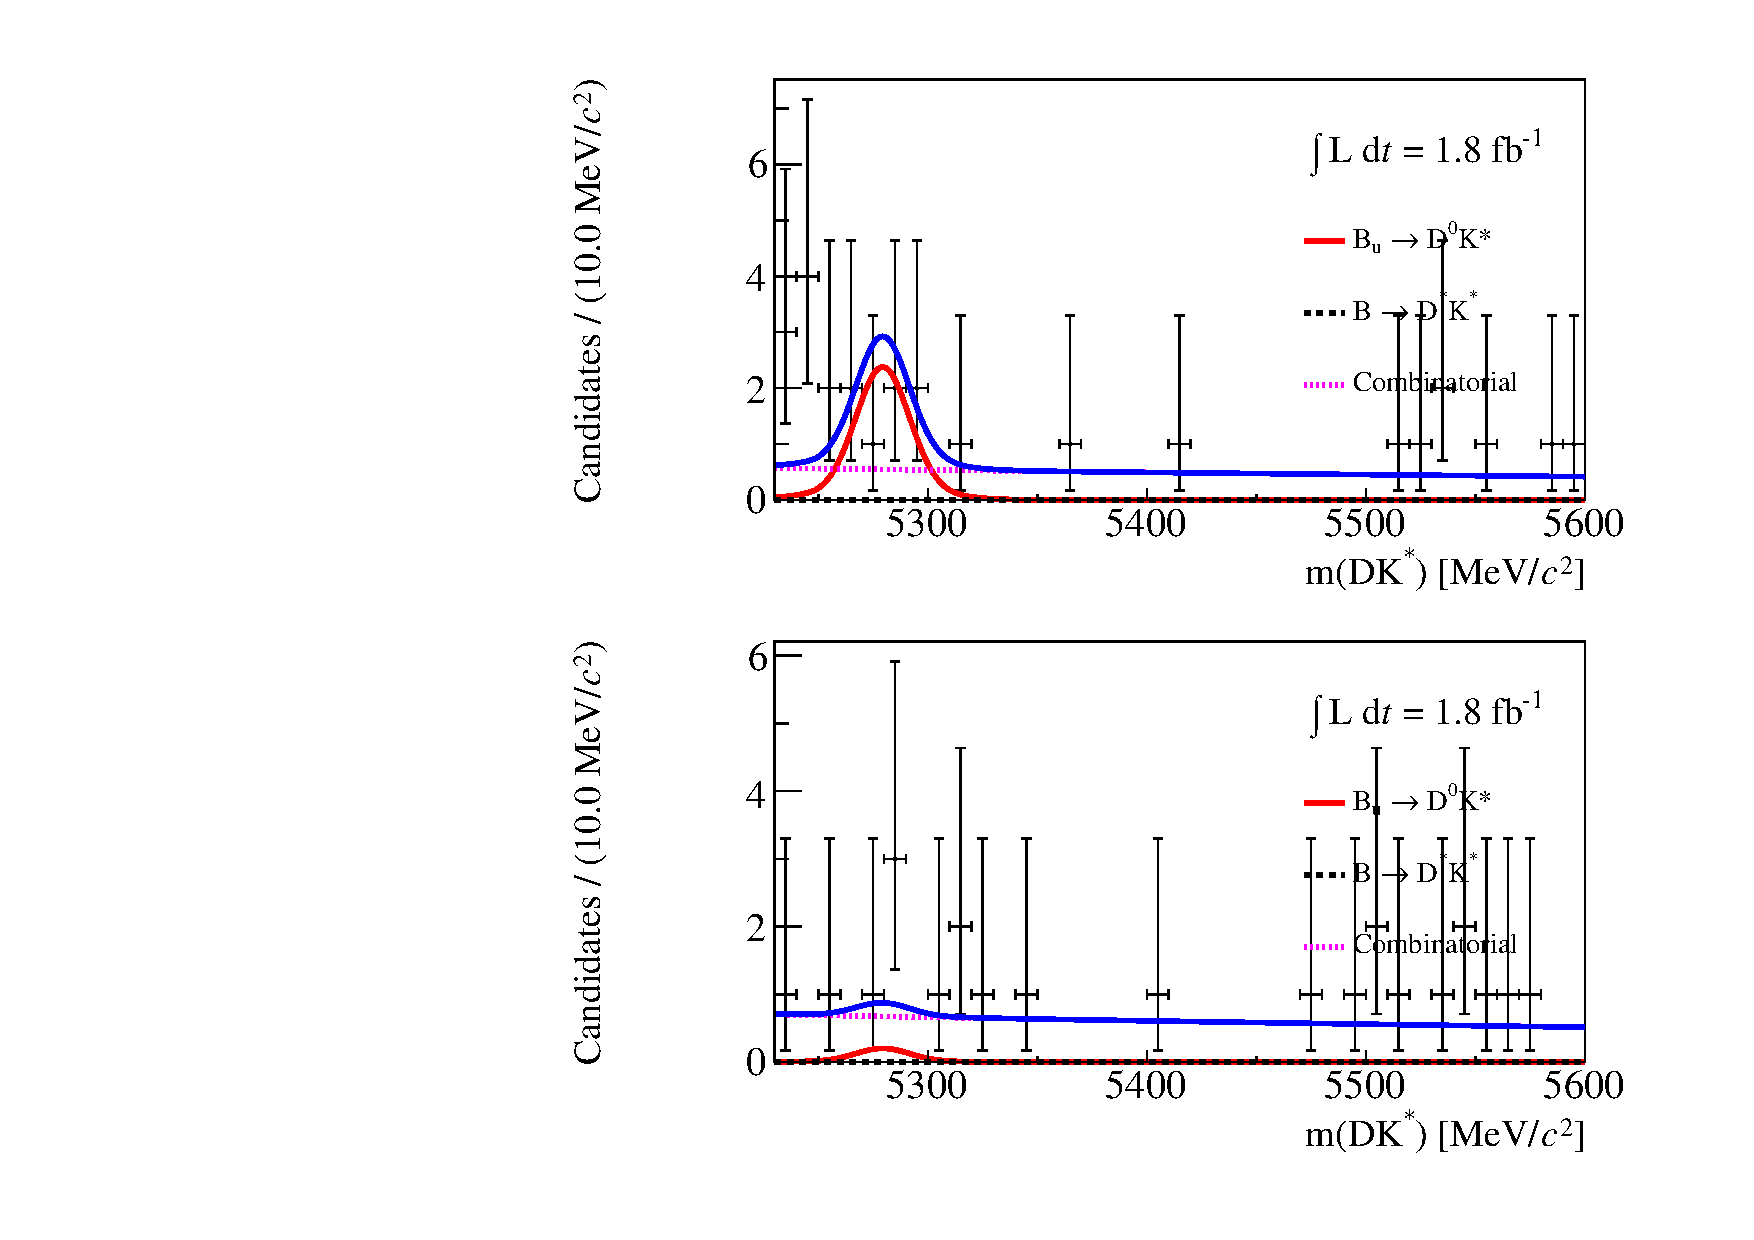
\includegraphics[trim = 0 0.5\imageheight{} 0 0,clip,width=0.5\linewidth]{figures/results/canvas_d2pik_DD_run2.pdf}
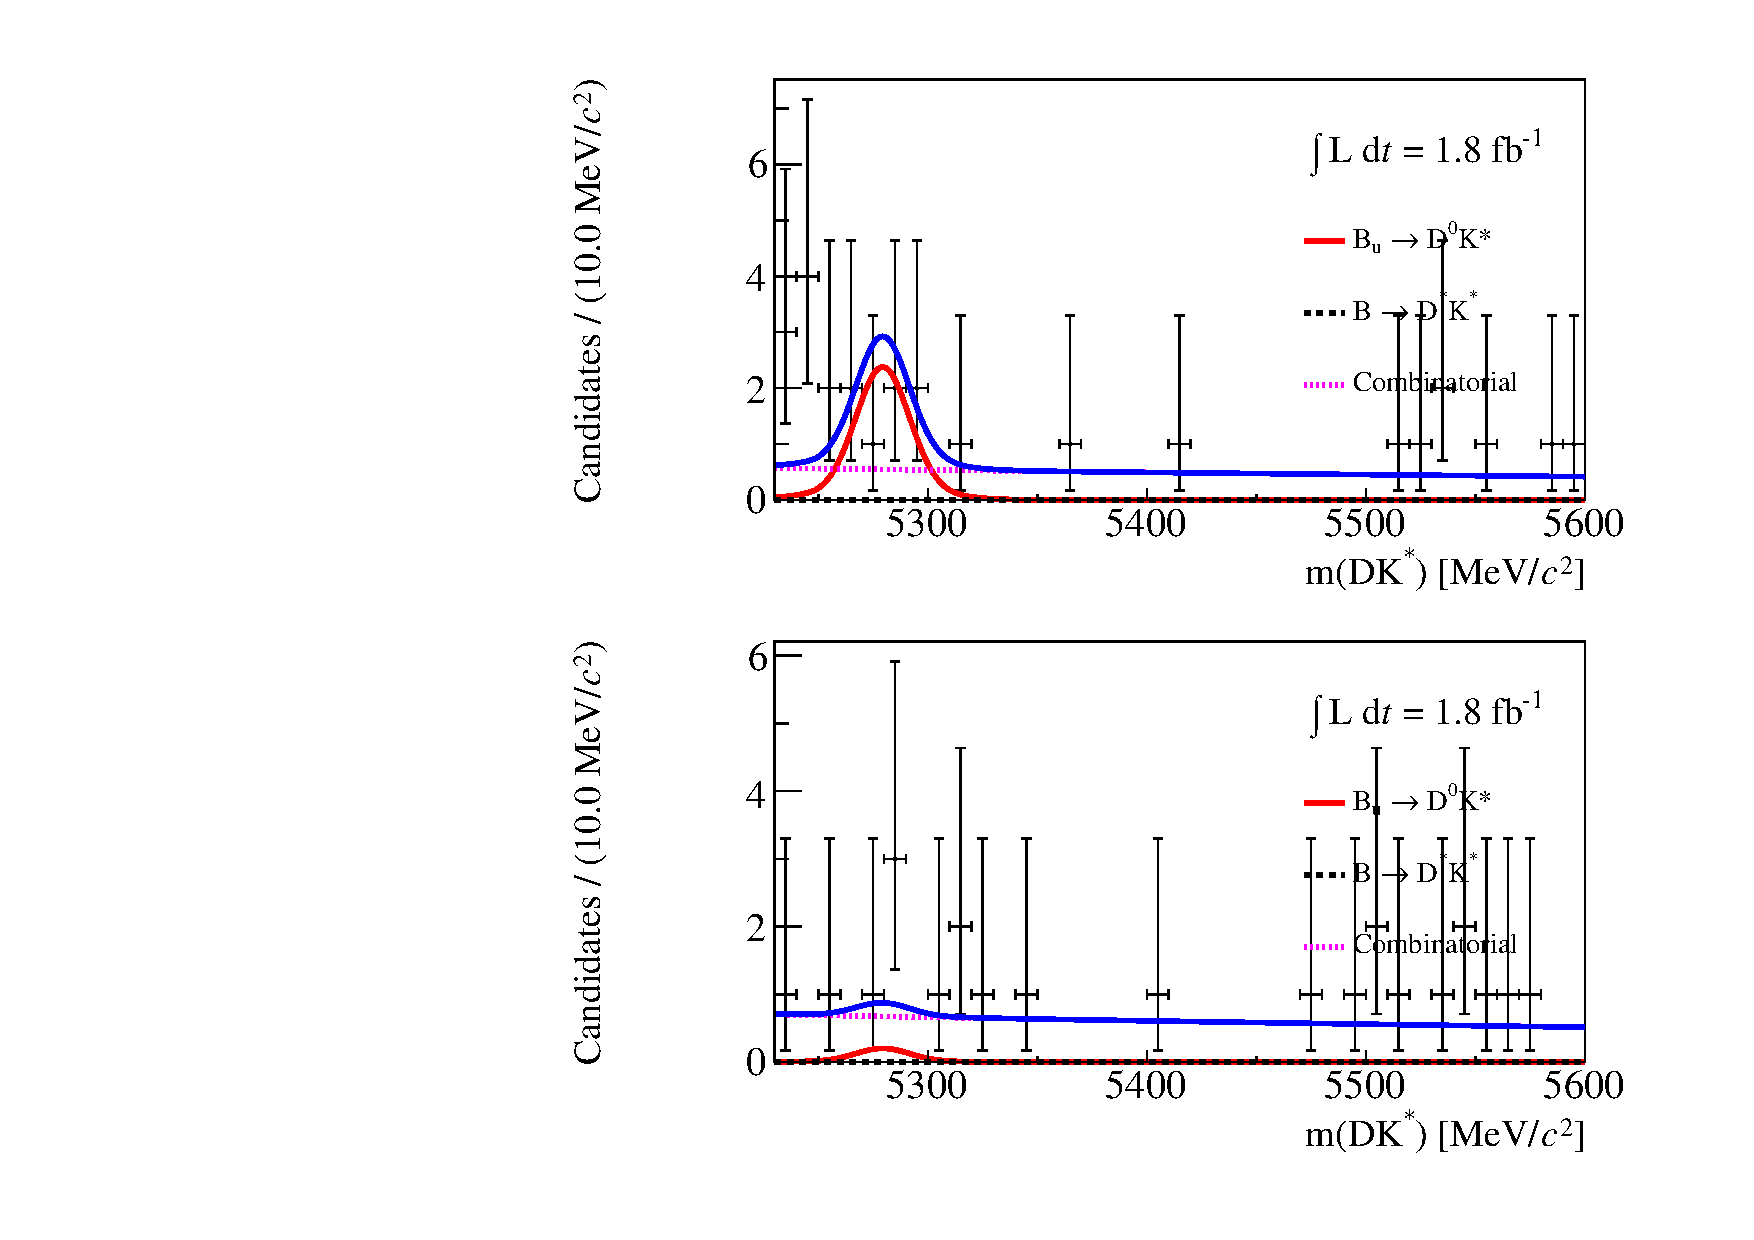
\includegraphics[trim = 0 0 0 0.5\imageheight{},clip,width=0.5\linewidth]{figures/results/canvas_d2pik_DD_run2.pdf}
\caption{Results of the simultaneous fit for the two-body modes, showing DD candidates in \runtwo data. In order from top to bottom, the plots show the \kpi, \kk, \pipi and \pik modes, for \Bp (left) and \Bm (right) decays.}
\label{results2body}
\end{figure}

\begin{figure}
\settoheight{\imageheight}{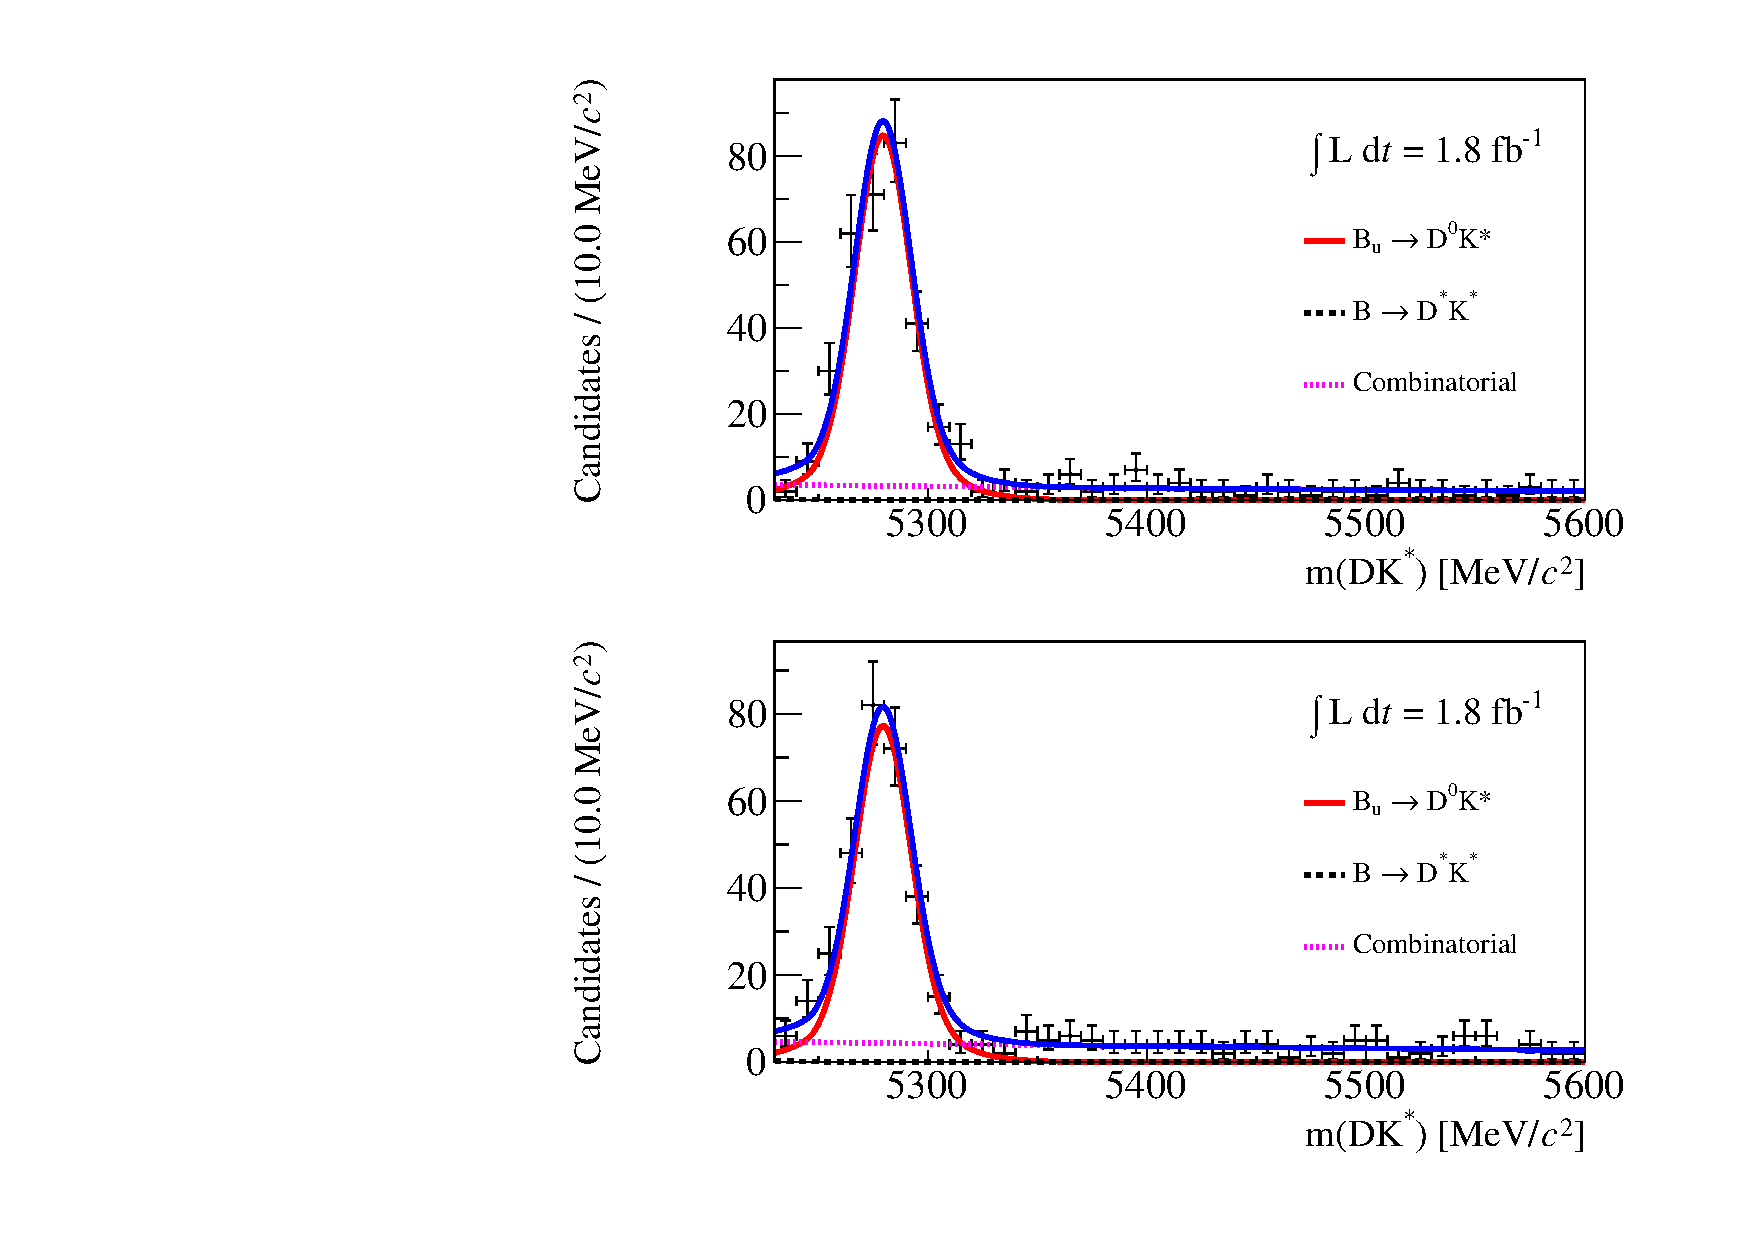
\includegraphics{figures/results/canvas_d2kpipipi_DD_run2.pdf}}
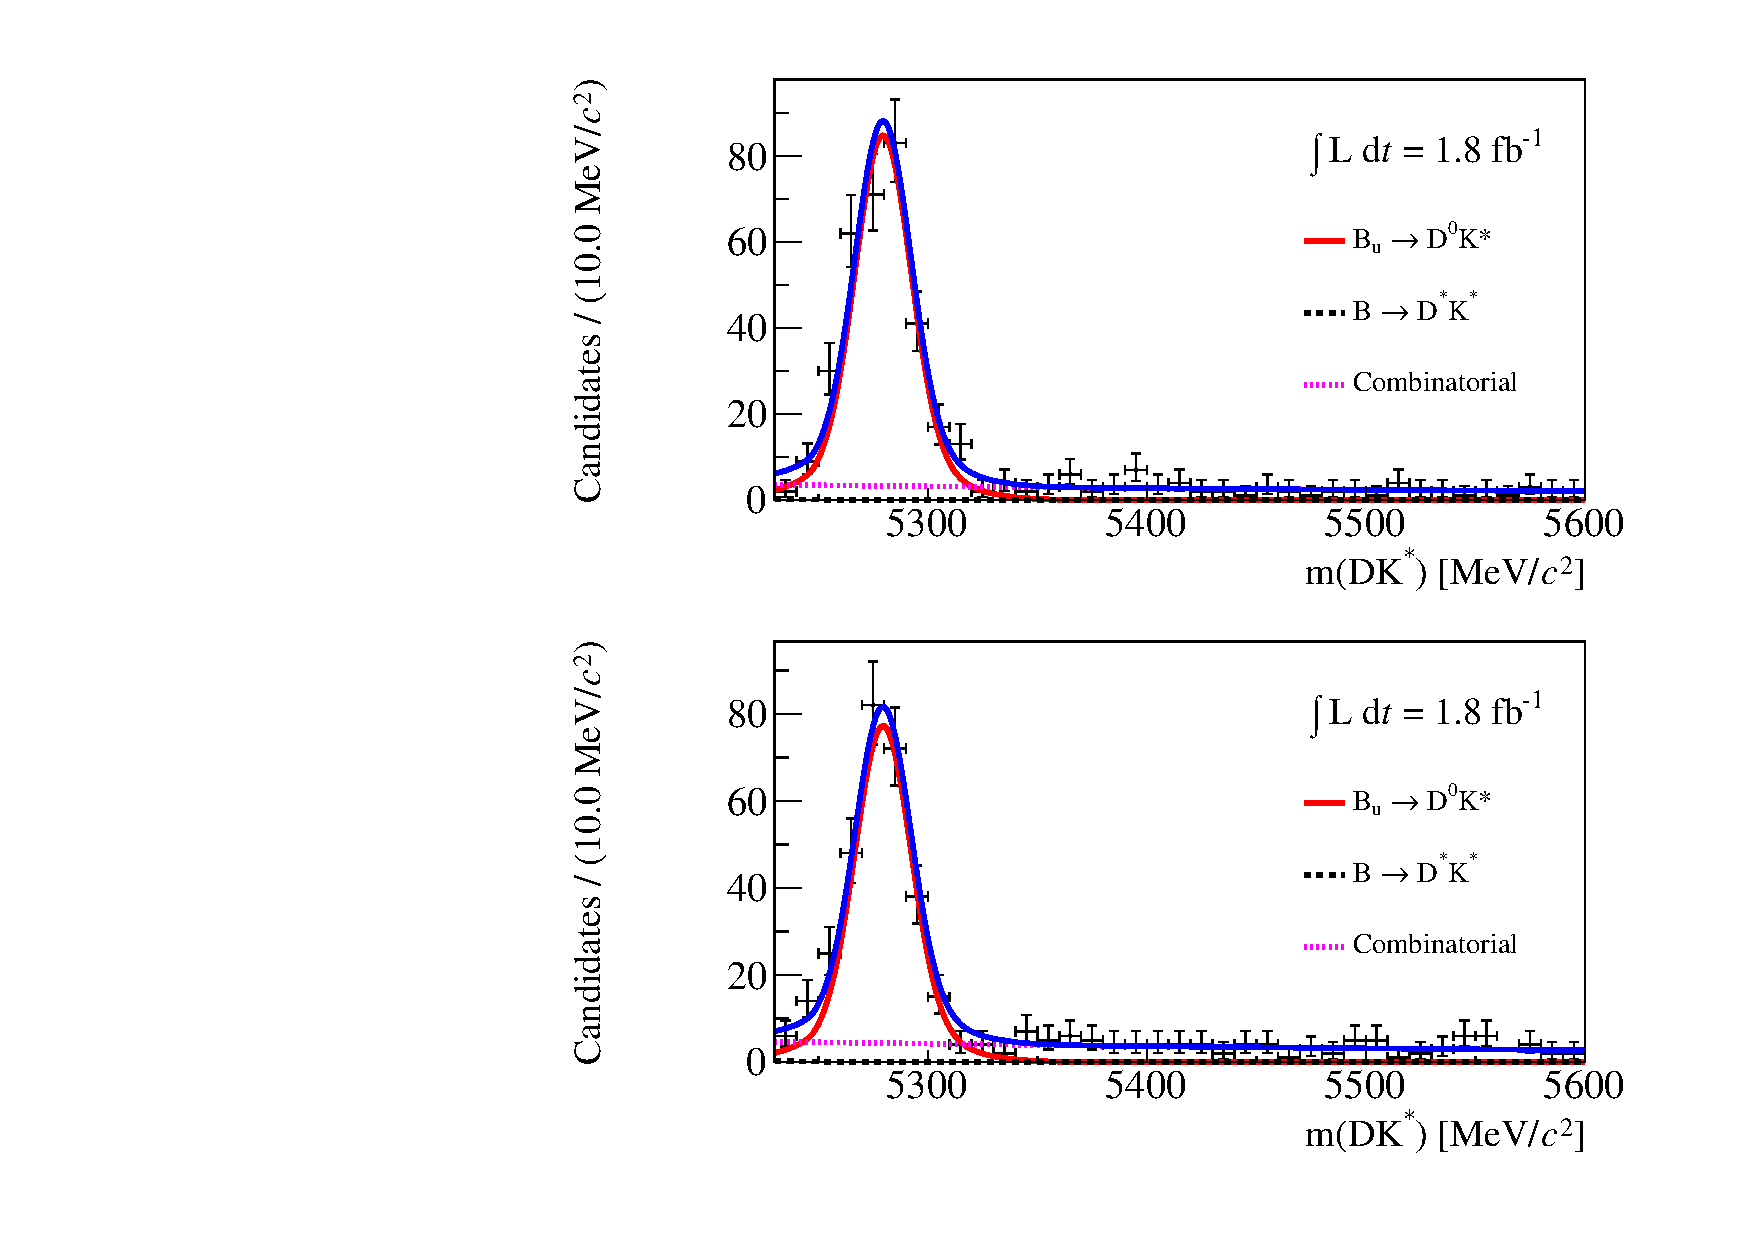
\includegraphics[trim = 0 0.5\imageheight{} 0 0,clip,width=0.5\linewidth]{figures/results/canvas_d2kpipipi_DD_run2.pdf}
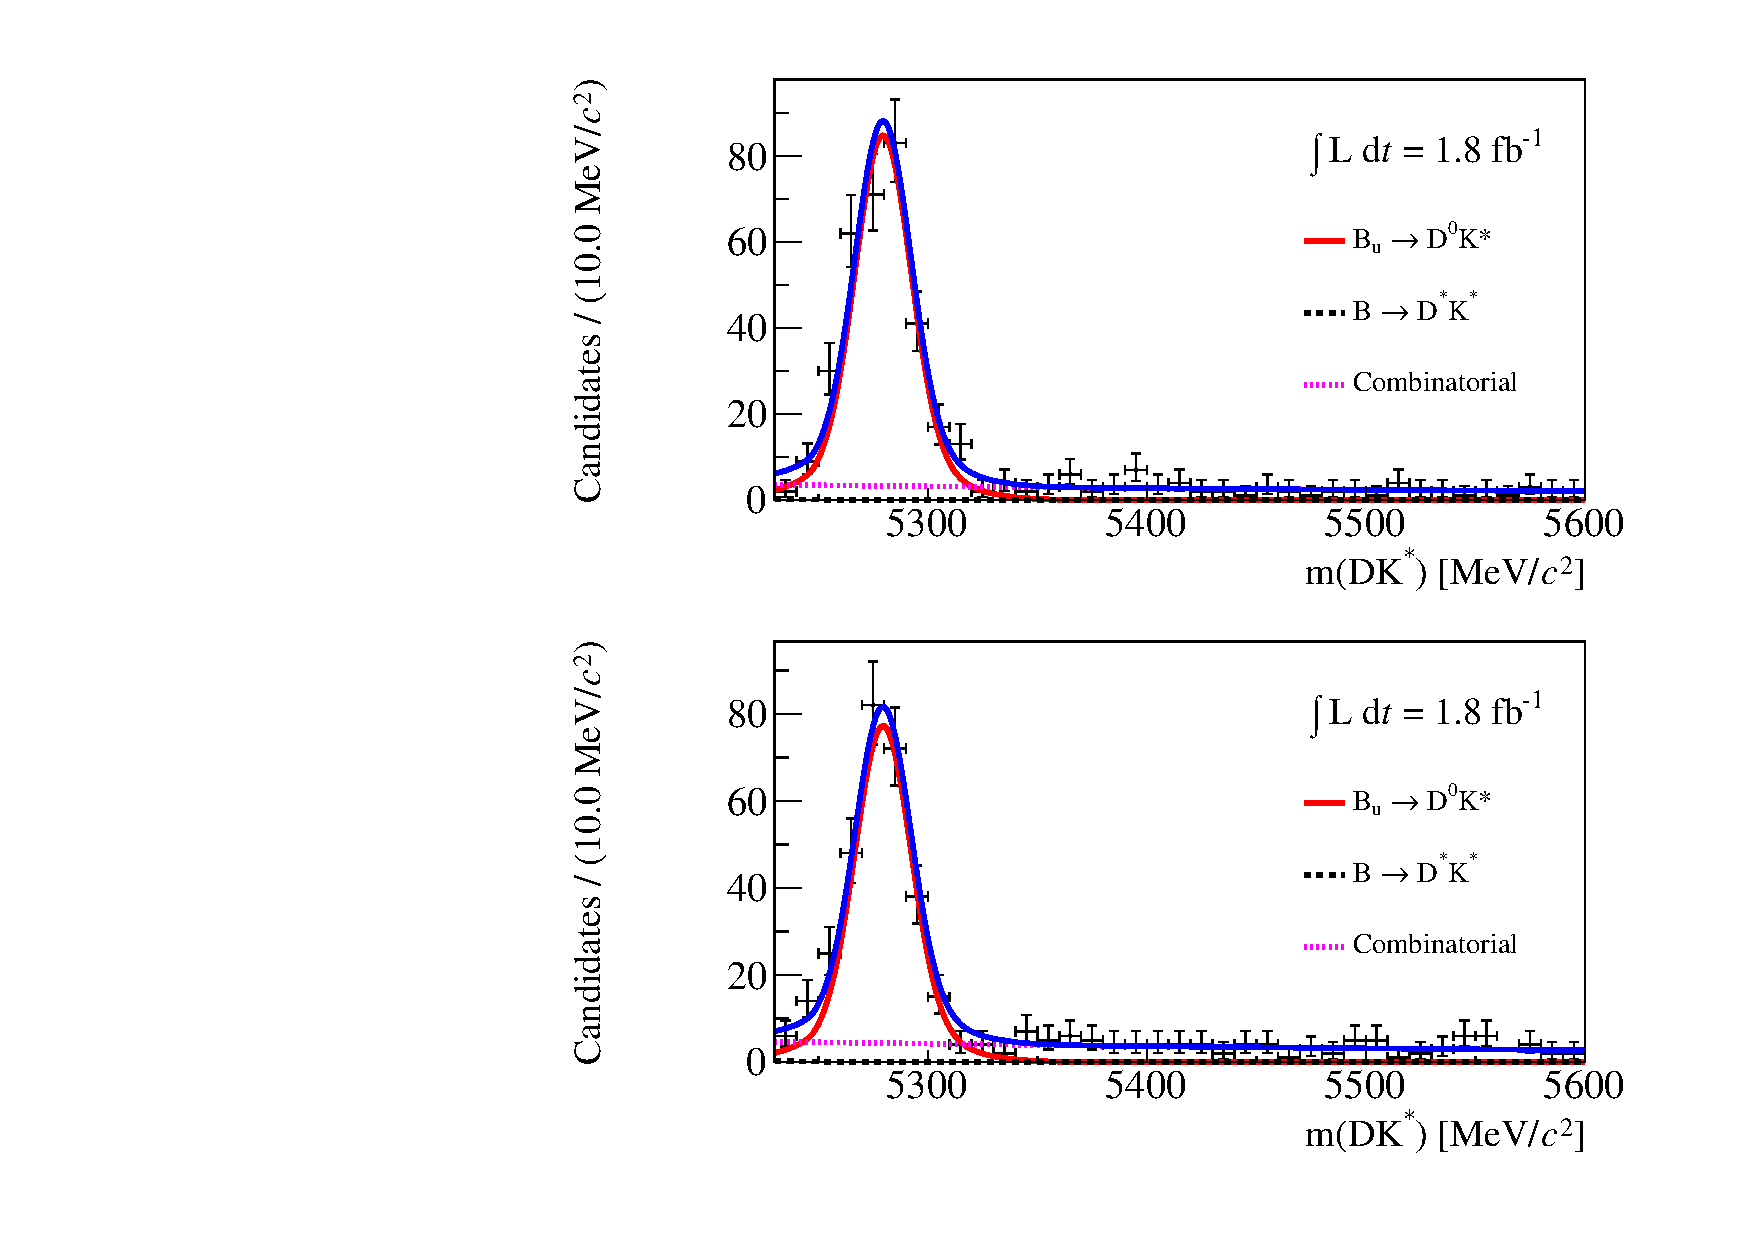
\includegraphics[trim = 0 0 0 0.5\imageheight{},clip,width=0.5\linewidth]{figures/results/canvas_d2kpipipi_DD_run2.pdf}
\hfill
\settoheight{\imageheight}{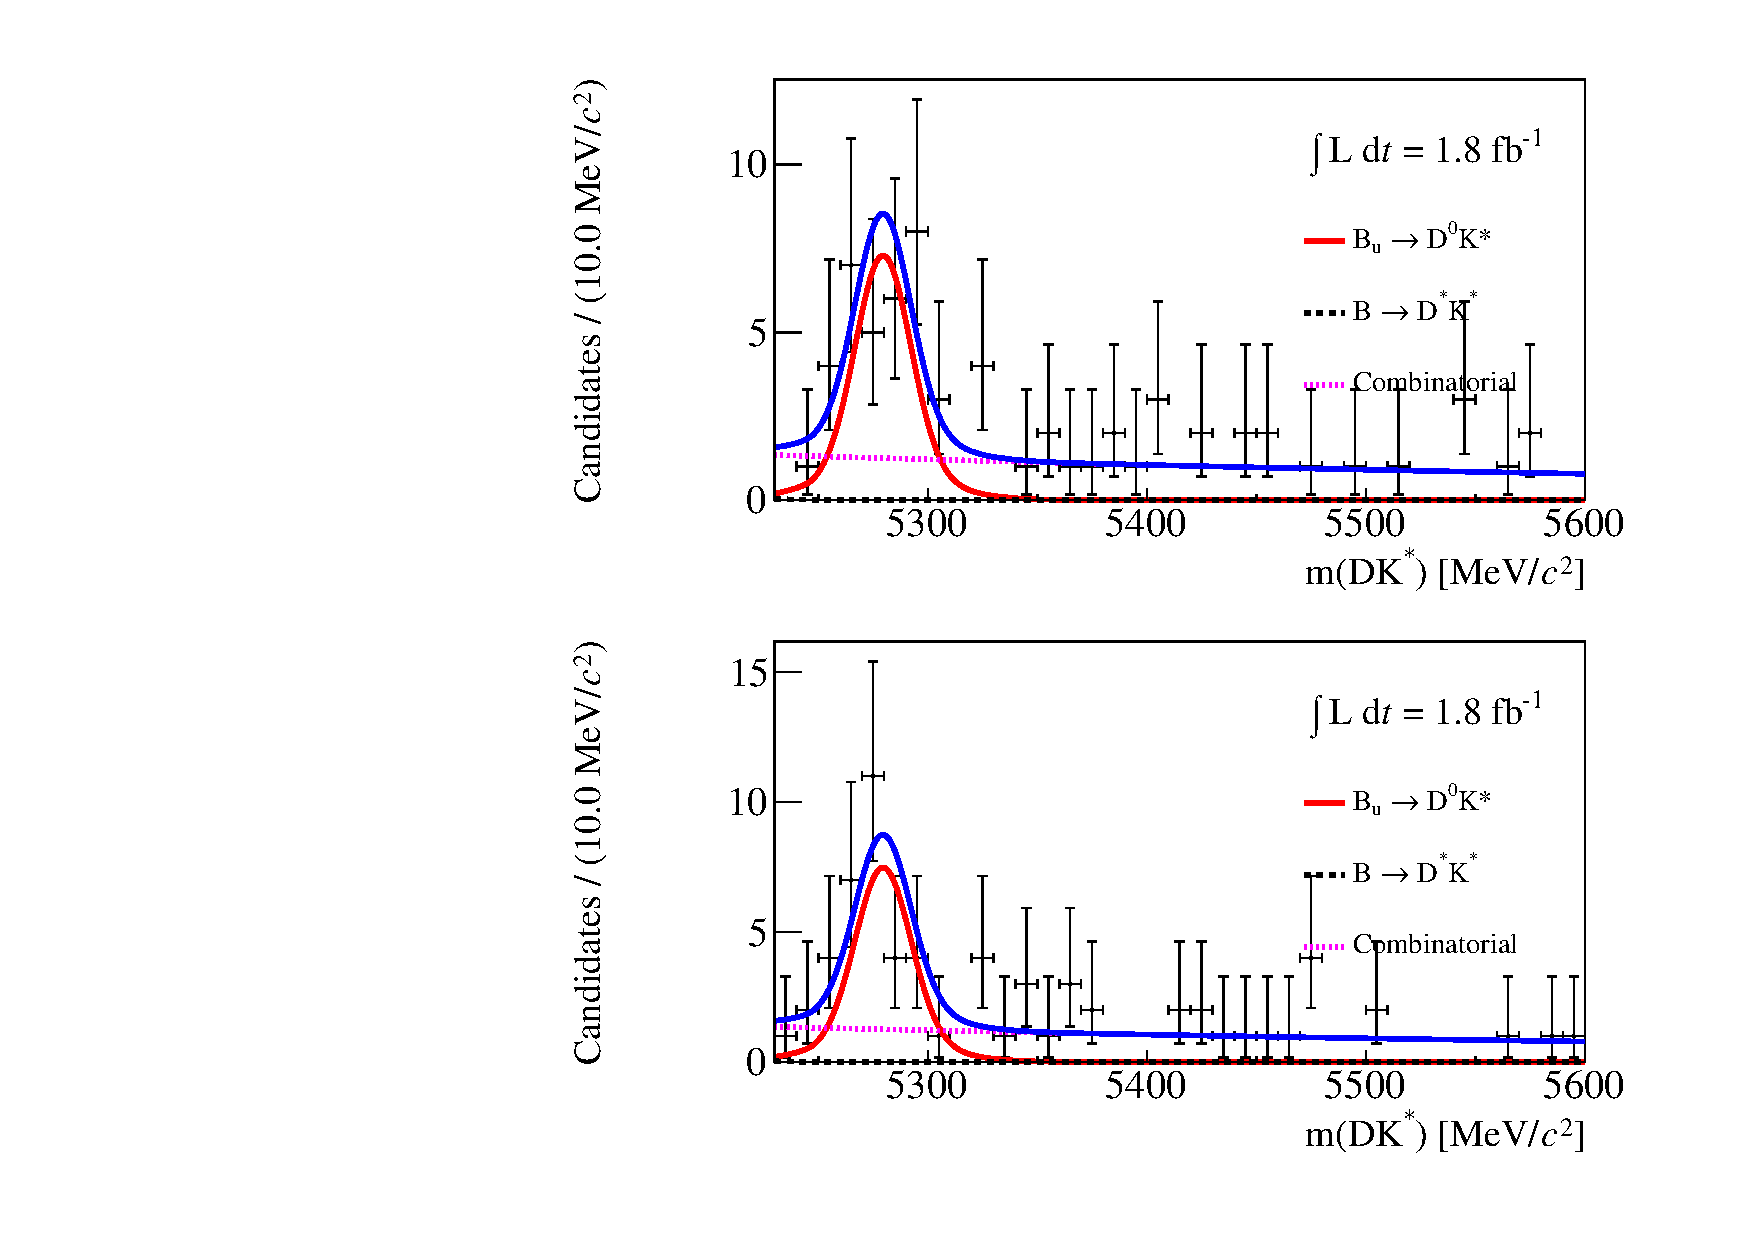
\includegraphics{figures/results/canvas_d2pipipipi_DD_run2.pdf}}
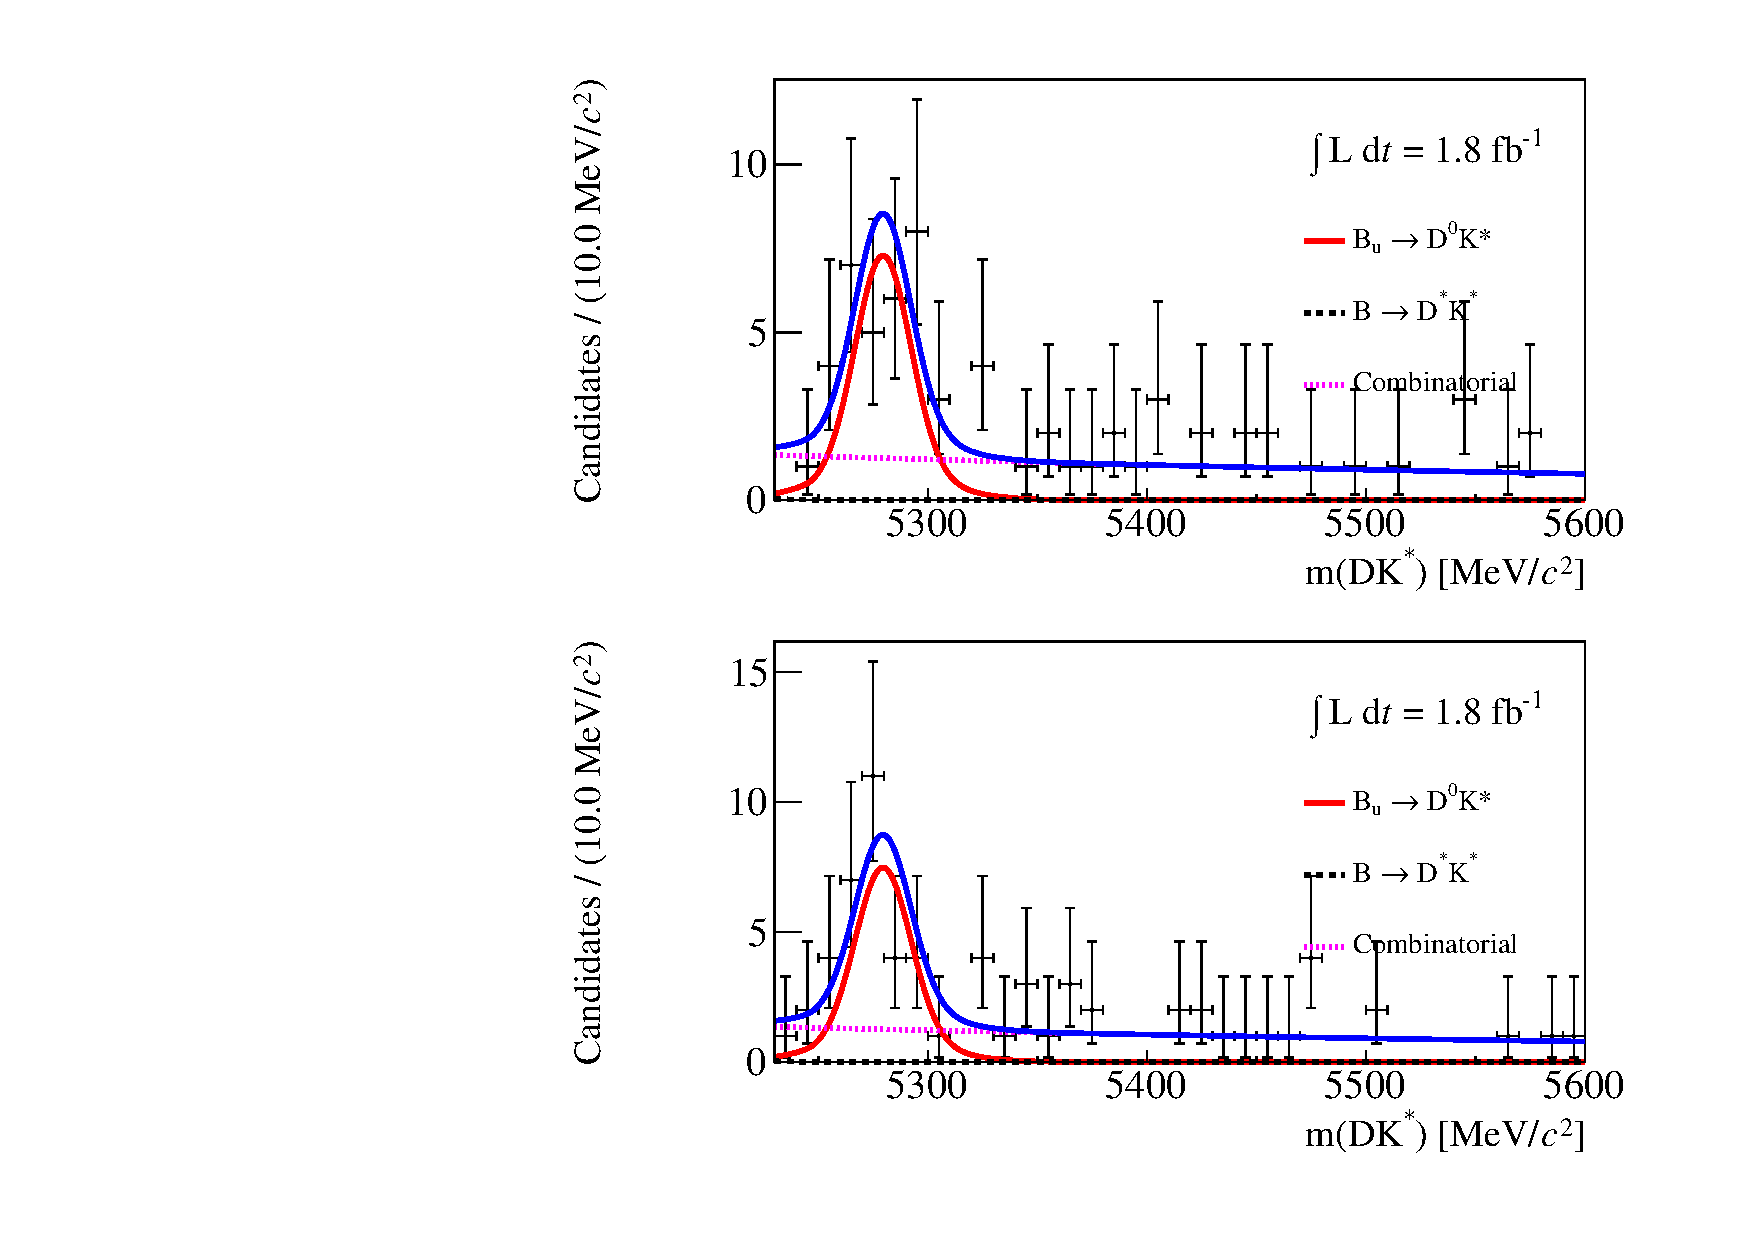
\includegraphics[trim = 0 0.5\imageheight{} 0 0,clip,width=0.5\linewidth]{figures/results/canvas_d2pipipipi_DD_run2.pdf}
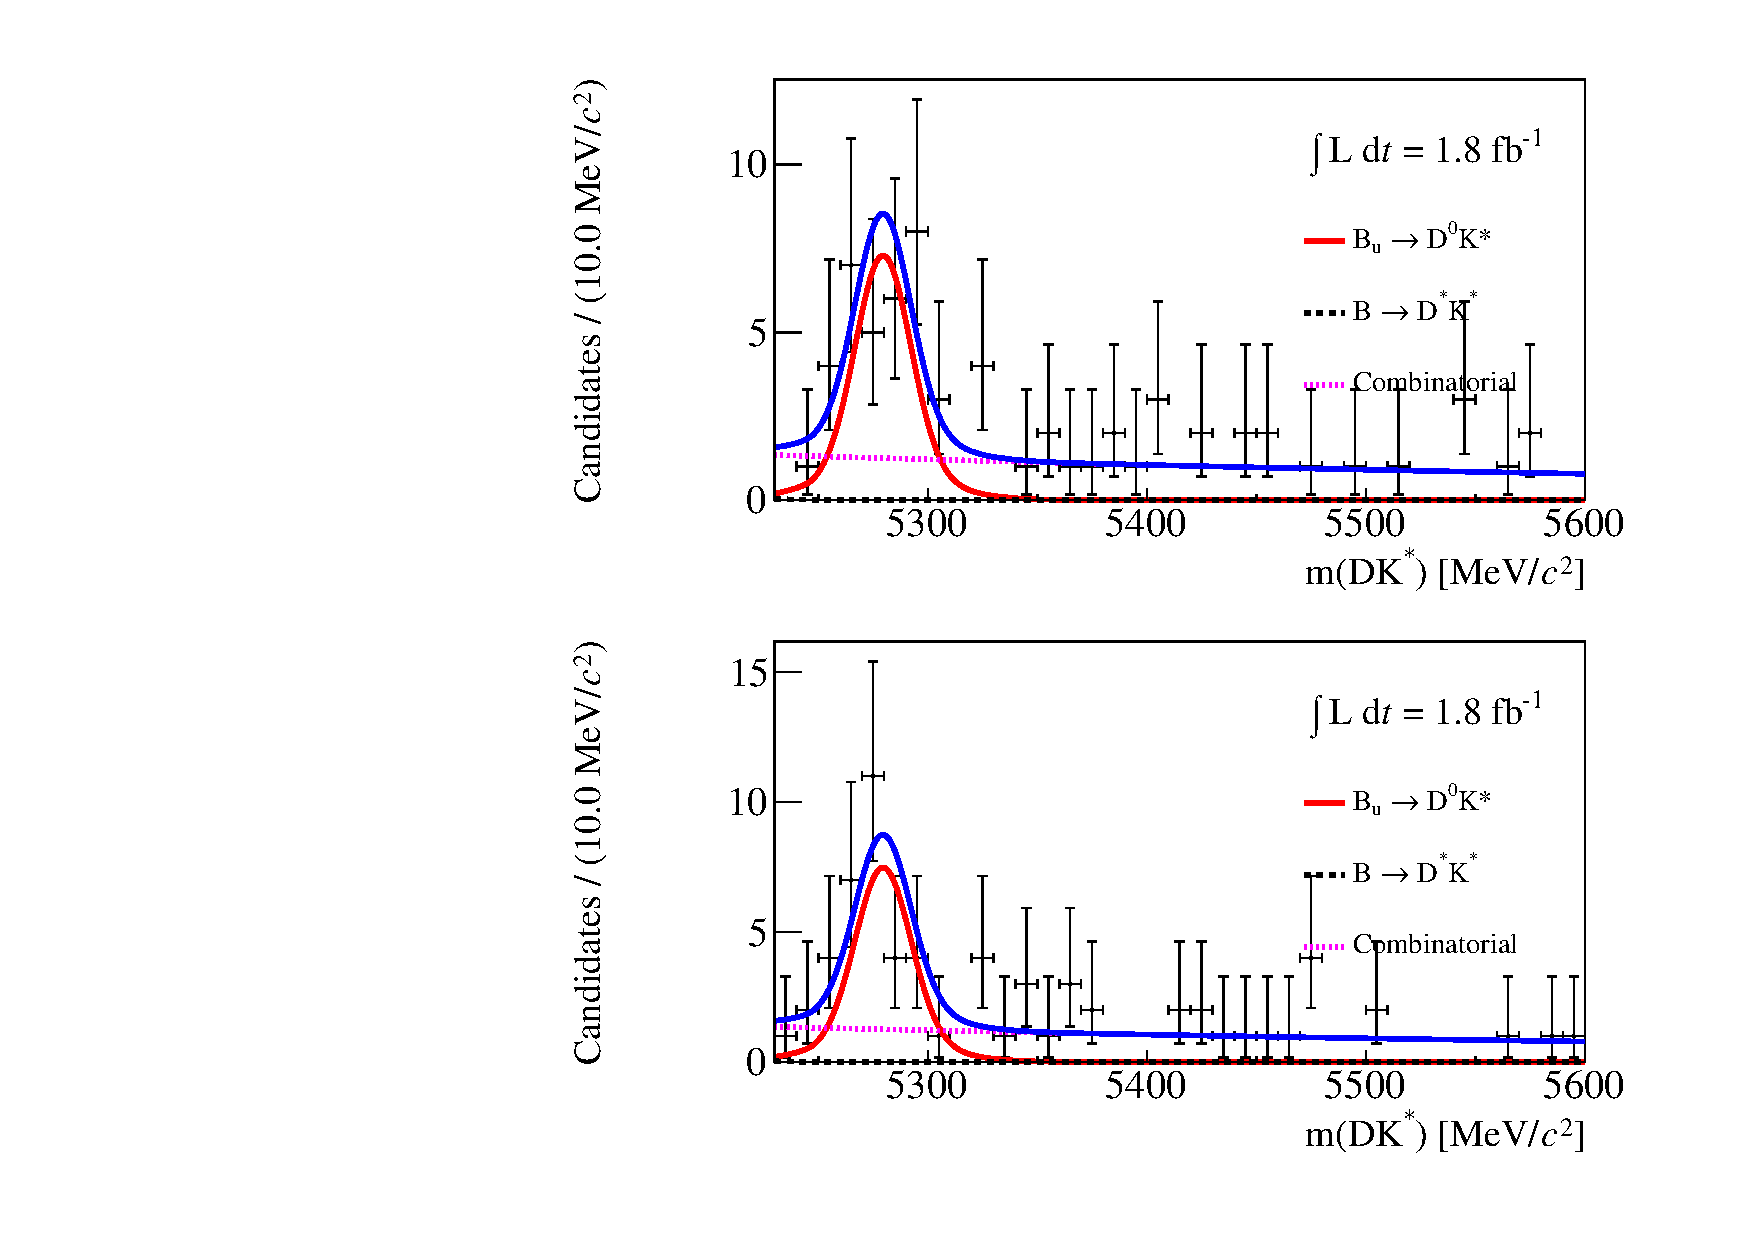
\includegraphics[trim = 0 0 0 0.5\imageheight{},clip,width=0.5\linewidth]{figures/results/canvas_d2pipipipi_DD_run2.pdf}
\hfill
\settoheight{\imageheight}{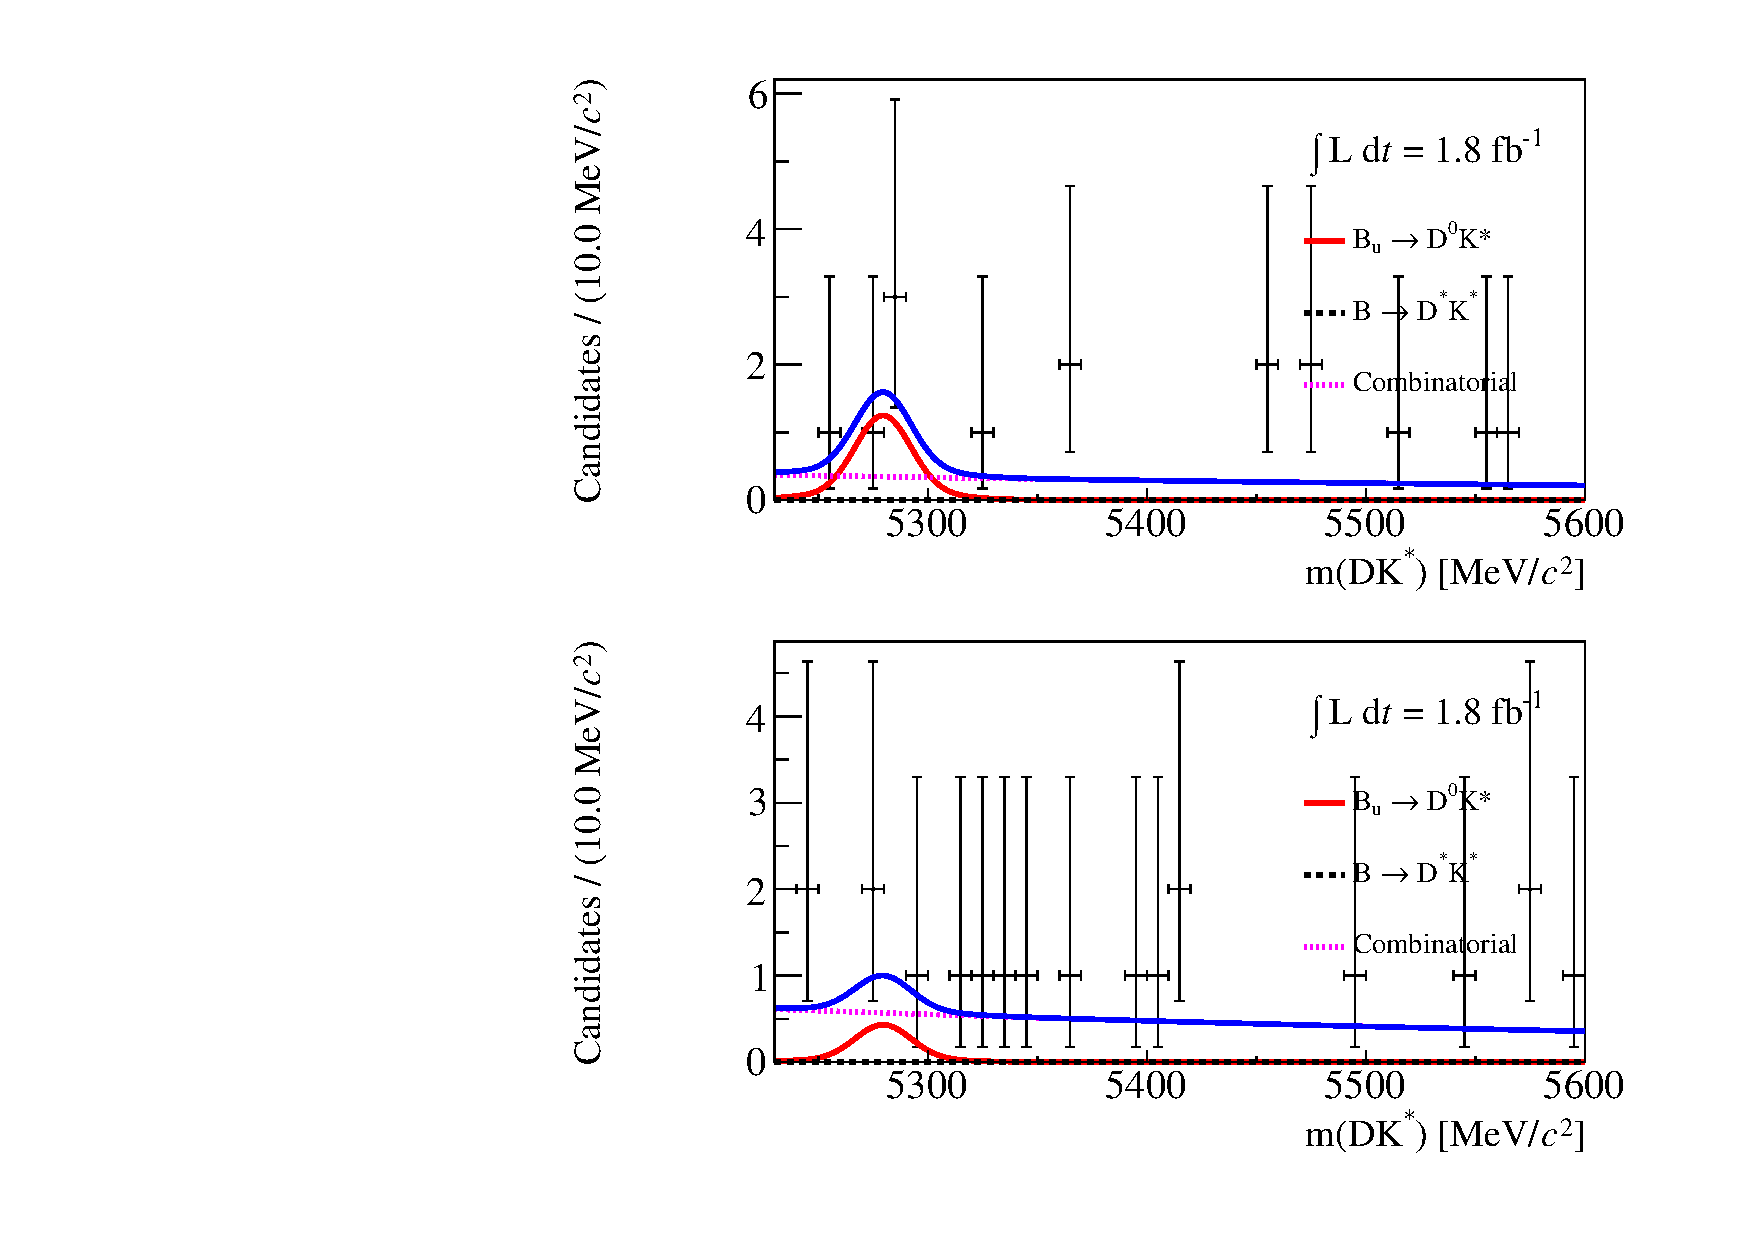
\includegraphics{figures/results/canvas_d2pikpipi_DD_run2.pdf}}
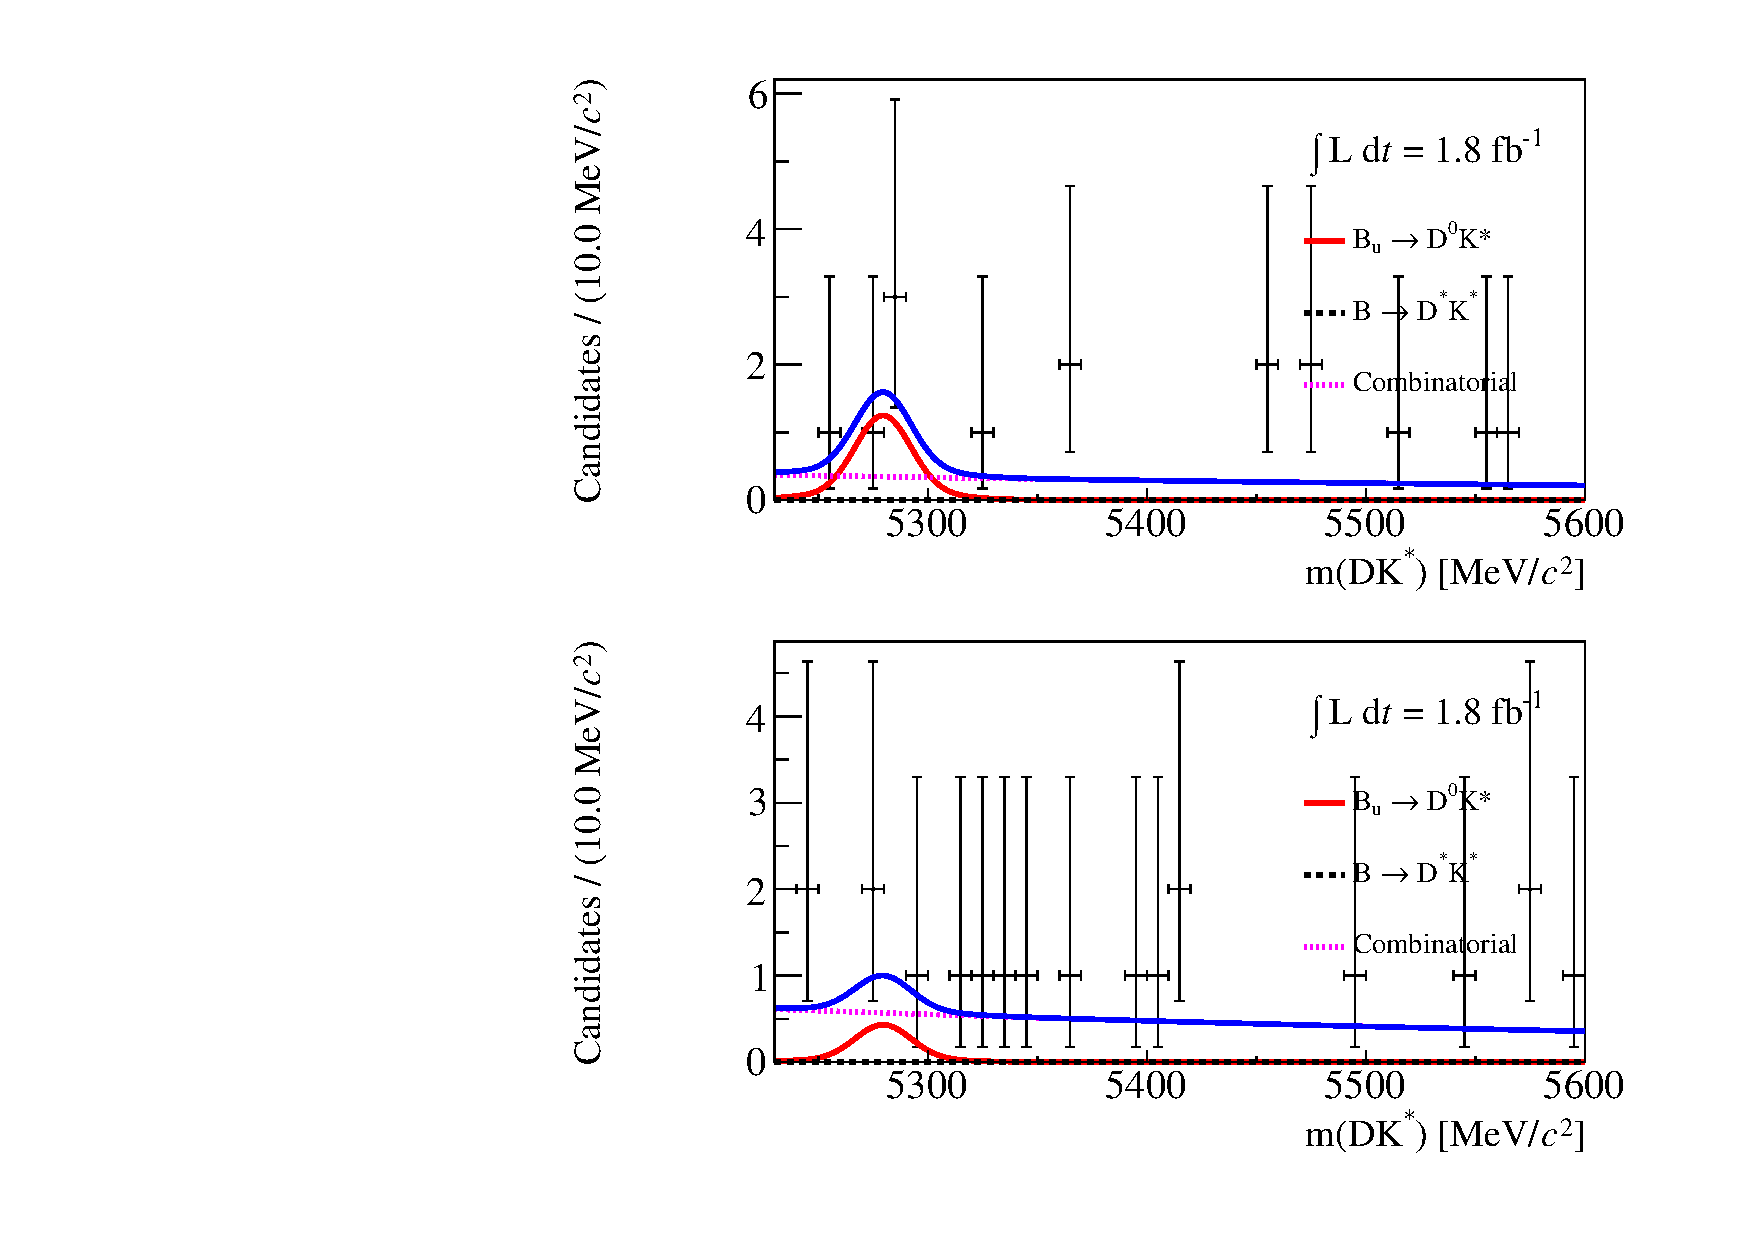
\includegraphics[trim = 0 0.5\imageheight{} 0 0,clip,width=0.5\linewidth]{figures/results/canvas_d2pikpipi_DD_run2.pdf}
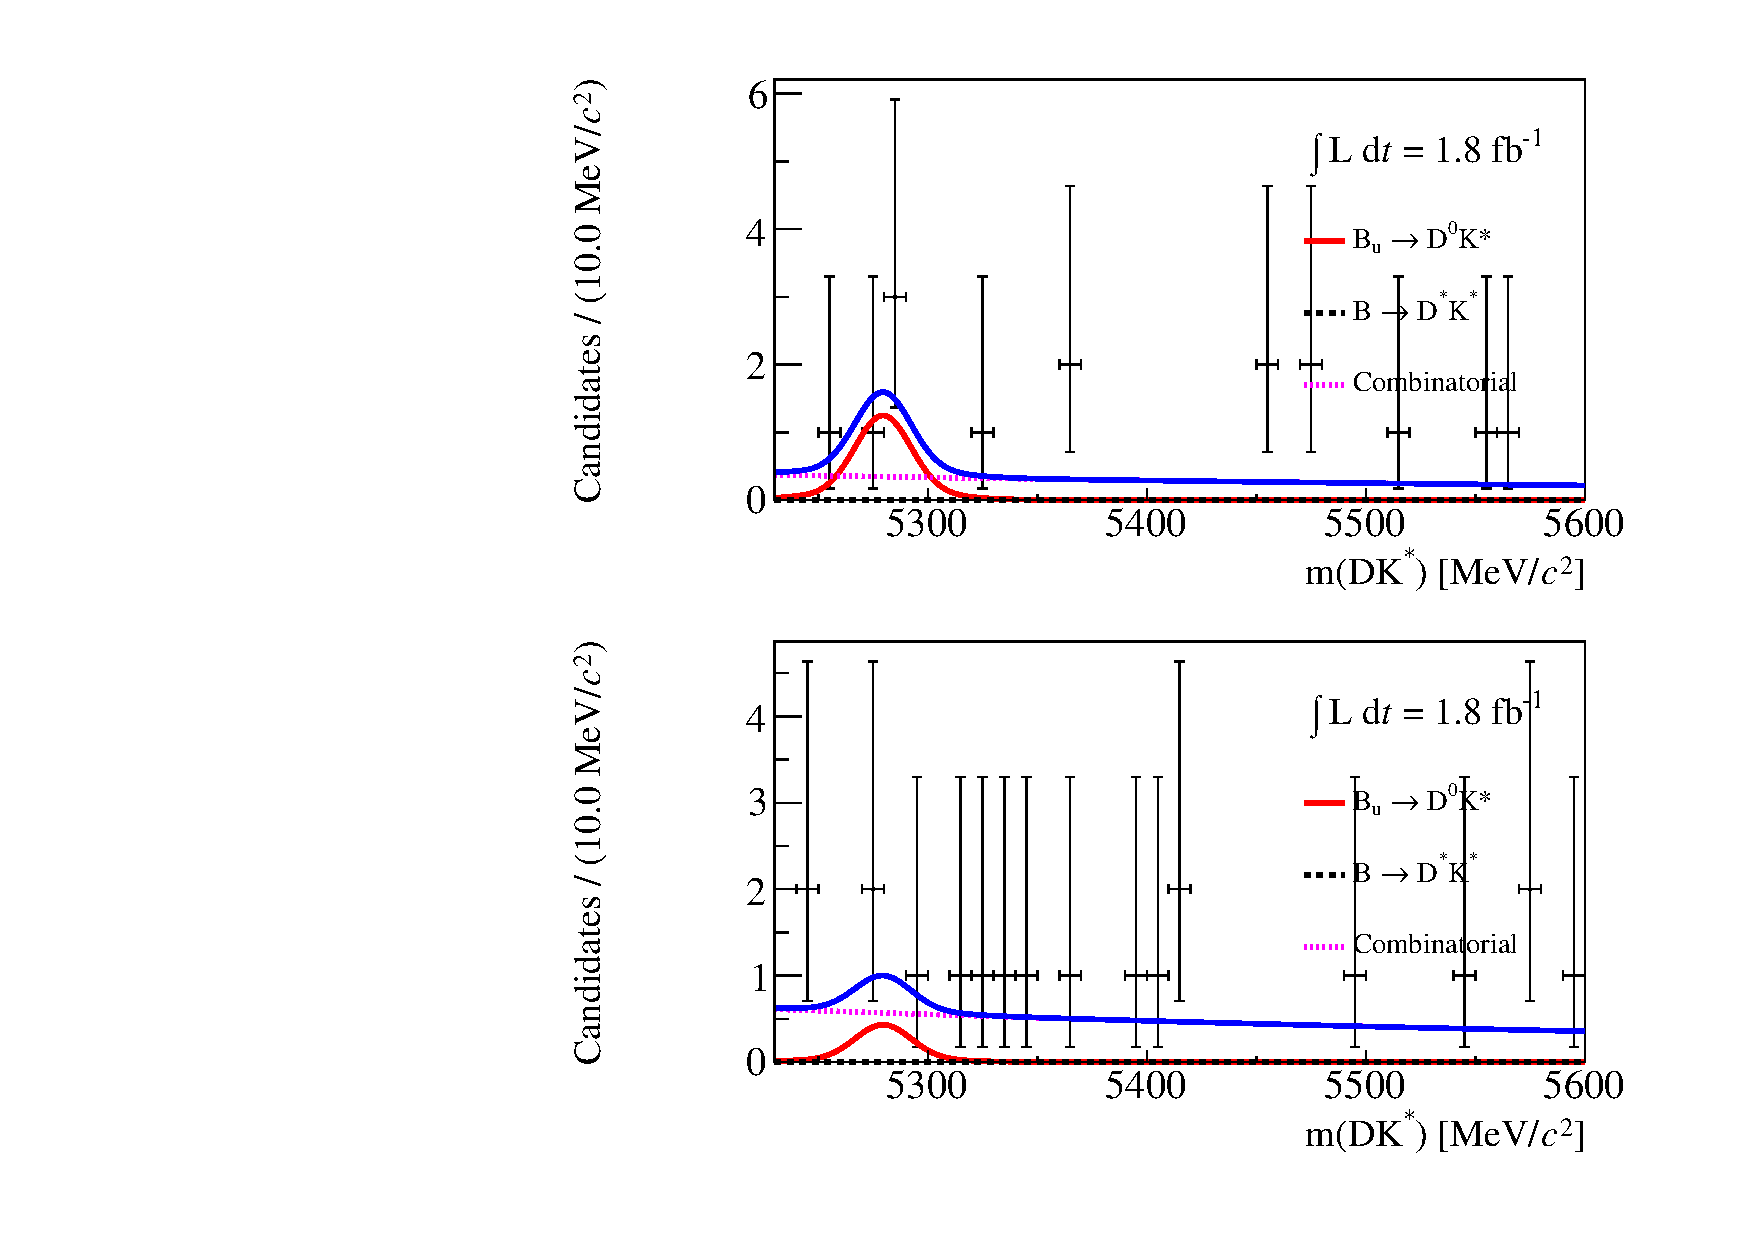
\includegraphics[trim = 0 0 0 0.5\imageheight{},clip,width=0.5\linewidth]{figures/results/canvas_d2pikpipi_DD_run2.pdf}
\caption{Results of the simultaneous fit for the four-body modes, showing DD candidates in \runtwo data. In order from top to bottom, the plots show the \kpipipi, \pipipipi and \pikpipi modes, for \Bp (left) and \Bm (right) decays.}
\label{results4body}
\end{figure}

\begin{table}[h]
\centering
{\footnotesize
\begin{tabular}{cccc}
Parameter & Fitted value & Negative uncertainty & Positive uncertainty \\
\hline
$A_{K\pi}$ & $-0.004$ & $-0.023$ & $0.023$ \\
$A_{KK}$ & $0.06$ & $-0.07$ & $0.07$ \\
$A_{\pi\pi}$ & $0.15$ & $-0.13$ & $0.13$ \\
$R_{KK}$ & $1.24$ & $-0.08$ & $0.09$ \\
$R_{\pi\pi}$ & $1.08$ & $-0.14$ & $0.15$ \\
$R^+_{K\pi}$ & $0.020$ & $-0.006$ & $0.006$ \\
$R^-_{K\pi}$ & $0.0018$ & $-0.0032$ & $0.0040$ \\
$A_{K\pi\pi\pi}$ & $-0.013$ & $-0.031$ & $0.031$ \\
$A_{\pi\pi\pi\pi}$ & $0.03$ & $-0.11$ & $0.11$ \\
$R_{\pi\pi\pi\pi}$ & $1.11$ & $-0.12$ & $0.13$ \\
$R^+_{K\pi\pi\pi}$ & $0.016$ & $-0.006$ & $0.008$ \\
$R^-_{K\pi\pi\pi}$ & $0.006$ & $-0.005$ & $0.006$ \\
\end{tabular}}
\caption{Fitted values of all the \CP parameters from the \CP fit.}
\label{cpfitresultsphysics}
\end{table}

\begin{table}[h]
\centering
{\footnotesize
\begin{tabular}{cccc}
Parameter & Fitted value & Negative uncertainty & Positive uncertainty \\
\hline
$N_{K\pi, DD, Run 1}$ & $503$ & $-22$ & $23$ \\
$N_{K\pi, DD, Run 2}$ & $911$ & $-32$ & $32$ \\
$N_{K\pi, LL, Run 1}$ & $228$ & $-14$ & $15$ \\
$N_{K\pi, LL, Run 2}$ & $388$ & $-19$ & $19$ \\
$N_{K\pi\pi\pi, DD, Run 1}$ & $233$ & $-15$ & $16$ \\
$N_{K\pi\pi\pi, DD, Run 2}$ & $560$ & $-26$ & $26$ \\
$N_{K\pi\pi\pi, LL, Run 1}$ & $101$ & $-9$ & $10$ \\
$N_{K\pi\pi\pi, LL, Run 2}$ & $251$ & $-16$ & $16$ \\
$\mu_{two-body}$ & $5279.4$ & $-0.3$ & $0.3$ \\
$\mu_{four-body}$ & $5279.5$ & $-0.5$ & $0.5$ \\
$\sigma_{two-body}$ & $12.1$ & $-0.3$ & $0.3$ \\
$\sigma_{four-body}$ & $12.6$ & $-0.4$ & $0.4$ \\
$\beta_{two-body, DD}$ & $-0.0008$ & $-0.0006$ & $0.0006$ \\
$\beta_{two-body, LL}$ & $0.0002$ & $-0.0011$ & $0.0012$ \\
$\beta_{four-body, DD}$ & $-0.0014$ & $-0.0006$ & $0.0006$ \\
$\beta_{four-body, LL}$ & $-0.0003$ & $-0.0014$ & $0.0015$ \\
\end{tabular}}
\caption{Fitted values of the signal yields and shape parameters from the \CP fit, where $\mu$ is the mean of the signal peak, $\sigma$ is the width of the signal peak and $\beta$ is the slope of the combinatorial background.}
\label{cpfitresultsshapes}
\end{table}

\begin{table}
\centering
\begin{tabular}{c|c}
\hline
Decay mode & Total signal yield \\
\hline
\kpi & $2030 \pm 49$ \\
\kk & $257 \pm 18$ \\
\pipi & $80 \pm 11$ \\
\pik & $20 \pm 7$ \\
\kpipipi & $1144 \pm 37$ \\
\pipipipi & $115 \pm 13$ \\
\pikpipi & $13 \pm 7$ \\
\hline
\end{tabular}
\caption{Total fitted yields in each of the \Dz decay modes extracted from the simultaneous fit performed with \Bm and \Bp charges combined.}
\label{fittedyields}
\end{table}


%%%%%%%%%%%%%%%%%%%%%%%%

\section{Systematics}
\label{sec:systematics}

When performing the \CP fit, uncertainty in the \CP observables arises from statistical fluctuations in the data due to the limited size of the data sample. These uncertainties, shown in Table \ref{cpfitresultsphysics}, are referred to as statistical uncertainty. However, there is a different source of uncertainty arising from the assumptions involved in the construction and implementation of the model, referred to as the systematic uncertainty. In this section, various sources of systematic uncertainty that affect the measurements of the \CP observables are investigated. For example, many fixed parameters are used in the fit model, and each of these fixed inputs has an associated uncertainty which needs to be propagated to the \CP observables. Also, uncertainties from the assumptions made for individual model components used in the \CP fit must also be propagated to the \CP observables. 

\subsection{Sources of systematic uncertainty}

Systematic uncertainties are calculated via two different methods. The method chosen in each case depends on the nature of the assumption being tested, as well as the information available. 

The first method (Method 1) involves determining the systematic uncertainty in data, whereby some input is adjusted. The value of the input drawn from a Gaussian distribution that has mean corresponding to the central value of the input and a width corresponding to the uncertainty in that value. Any correlations between the parameters are ignored. Each time the \CP fit is performed a value for each of the fitted parameters is extracted, resulting in a distribution for each \CP observable. The standard deviation of each of these distributions is taken to be the systematic uncertainty for that \CP observable. Sources of systematic uncertainty calculated via this method are those that arise due to the use of fixed inputs in the \CP fit, from branching ratios, simulation efficiencies, asymmetry corrections and shape parameters. This method aims to quantify how much the \CP observables are affected by changes to these inputs on the scale of their associated uncertainty.

The second method (Method 2) involves estimating the systematic uncertainty using pseudoexperiments, as described in Section \ref{sec:cpfit:optimisation}. For each of these systematic effects being investigated, the generated model is varied to account for the corresponding model assumption. The systematic uncertainty on each observable is taken to be the difference between the mean of the fitted parameter distribution from pseudoexperiments and the generated value. Sources of systematic uncertainty calculated via this method are those that occur due to the modelling of various components in the \CP fit, namely the choice in modelling signal and partially reconstructed backgrounds, the effect of any residual charmless \B decays, the uncertainty in the modelling of the \decay{\Lb}{\Lc(p\kaon\pi)\Kstarm} background and the effect of any possible contribution from \decay{\Bs}{\Dzb\bar{K}^{*}(1410)^0} decays.

Each of the sources of systematic uncertainty, from both fixed inputs and model components, is described individually in the following sections. A summary of the systematic uncertainties for the \CP observables is given in Table~\ref{systematics}.

\subsubsection{Branching ratios}

The branching ratios for the different \Dz decays are used in the \CP fit as shown in Equations \ref{effcorrectionglw2body} and \ref{effcorrectionglw4body}. Table \ref{BR} gives the values of the branching ratios along with their uncertainties. The systematic uncertainty due to using the branching ratios as fixed inputs in the \CP fit is calculated using Method 1, where the uncertainties in the branching ratios are used as the scale of the variation in the corresponding input.

\begin{table}
\centering
\begin{tabular}{l|l}
\hline
Mode & Branching ratio \\
\hline
$\mathcal{B}(\decay{\Dz}{\Km\pip})$ & $0.0393 \pm 0.0004$ \\
$\mathcal{B}(\decay{\Dz}{\Kp\Km})$ & $0.00401 \pm 0.00007$ \\
$\mathcal{B}(\decay{\Dz}{\pip\pim})$ & $0.001421 \pm 0.000025$ \\
$\mathcal{B}(\decay{\Dz}{\Km\pip\pim\pip})$ & $0.0811 \pm 0.0015$ \\
$\mathcal{B}(\decay{\Dz}{\pip\pim\pip\pim})$ & $0.00745 \pm 0.00020$ \\
\hline
\end{tabular}
\caption{Branching ratios for the different \Dz decay modes, which are used as fixed inputs in the \CP fit~\cite{PDG2014}.}
\label{BR}
\end{table}

\subsubsection{Simulation efficiencies}

Selection efficiencies and BDT efficiencies are used in the \CP fit as shown in Equations \ref{effcorrectionglw2body}, \ref{effcorrectionglw4body}, \ref{effcorrectionads2body} and \ref{effcorrectionads4body}. The values used in the \CP fit are shown in Tables \ref{seleff} and \ref{bdteff} along with their uncertainties. The systematic uncertainty, due to using the efficiencies as fixed values in the \CP fit, is calculated using Method 1, where the uncertainties in the efficiencies are used as the scale of the variation.

\subsubsection{PID efficiencies}

PID efficiencies are used as fixed inputs in the \CP fit as shown in Equations \ref{effcorrectionglw2body} and \ref{effcorrectionglw4body} and the values used are shown in Table \ref{pideff}. The systematic uncertainty is calculated using Method 1, where the uncertainties in the efficiencies are used as the scale of the variation.

\subsubsection{Veto efficiencies}

Veto efficiencies are required in the \CP fit to correct for the veto applied in the two- and four-body ADS modes, as shown in Equations \ref{effcorrectionads2body} and \ref{effcorrectionads4body}, with the actual values used shown in Table \ref{vetoeff} along with their uncertainties. The systematic uncertainty, due to using these values as fixed inputs in the \CP fit, is calculated using Method 1, where the uncertainties in the efficiencies are used as the scale of the variation.

\subsubsection{Asymmetry corrections}

Corrections must be made in the \CP fit for various sources of asymmetry as detailed in Section \ref{sec:cpfit:asymmetries}, namely production asymmetry, detection asymmetry and PID asymmetry. For each source of asymmetry a correction is applied in the \CP fit and a systematic is assigned separately to each based on the uncertainty of each correction using Method 1. 

For the production asymmetry, a \runone value is extracted using measurements performed with \decay{\Bp}{\Dzb\pip} decays~\cite{LHCb-PAPER-2016-054} in data. The equivalent results for \runtwo data are not currently available, therefore the production asymmetry for \runtwo is taken to have the same central value as \runone with twice the uncertainty, which is considered sufficient to cover any unknown difference in the production asymmetry due to the increased centre-of-mass energy. For the detection asymmetry, the corrections are obtained using \runone data, but the same results are used for \runtwo data. The changes to the detector between the data-taking periods are not expected to significantly affect the detection asymmetry measurement. For the PID asymmetry, the corrections are calculated separately for \runone and \runtwo, and are used as fixed inputs in the \CP fit. In each case, the uncertainties are used as the scale of the variation for calculating the systematic uncertainty.

\subsubsection{Signal shape}
\label{sec:systematics:signal}

The signal shape, described in Section \ref{sec:massfit:signal}, is modelled as a Double Crystal Ball with all the parameters fixed from simulation apart from the mean and width. From simulated signal samples it can be seen that the signal shape has more than one characteristic width and a low mass tail. There are two sources of uncertainty in the choice of signal shape: the tail parameters, $\alpha$ and $n$, and the width ratio and yield fraction, $f_{\sigma}$ and $f_{cb}$ respectively, between the two CBs. These two sources of uncertainty are treated separately and combined. The uncertainty in the tail parameters is quantified using Method 2, by using an alternative signal shape, formed from the sum of two Gaussian-like distributions with a common mean, different widths and two other parameters relating to the skewness and sharpness of the distribution~\cite{doublejohnson}. This shape is taken to have the same width ratio and yield fraction as the Double Crystal Ball used in the \CP fit. Other parameters are fixed from a maximum likelihood fit to the simulated signal sample, shown in Figure \ref{signalshapesys}. The \CP fit is then performed to this data, generated with this alternative shape, using the nominal fit model.  The results from this method are given in the first row of Table \ref{signalshapeSystematics}.

\begin{figure}[h]
\centering
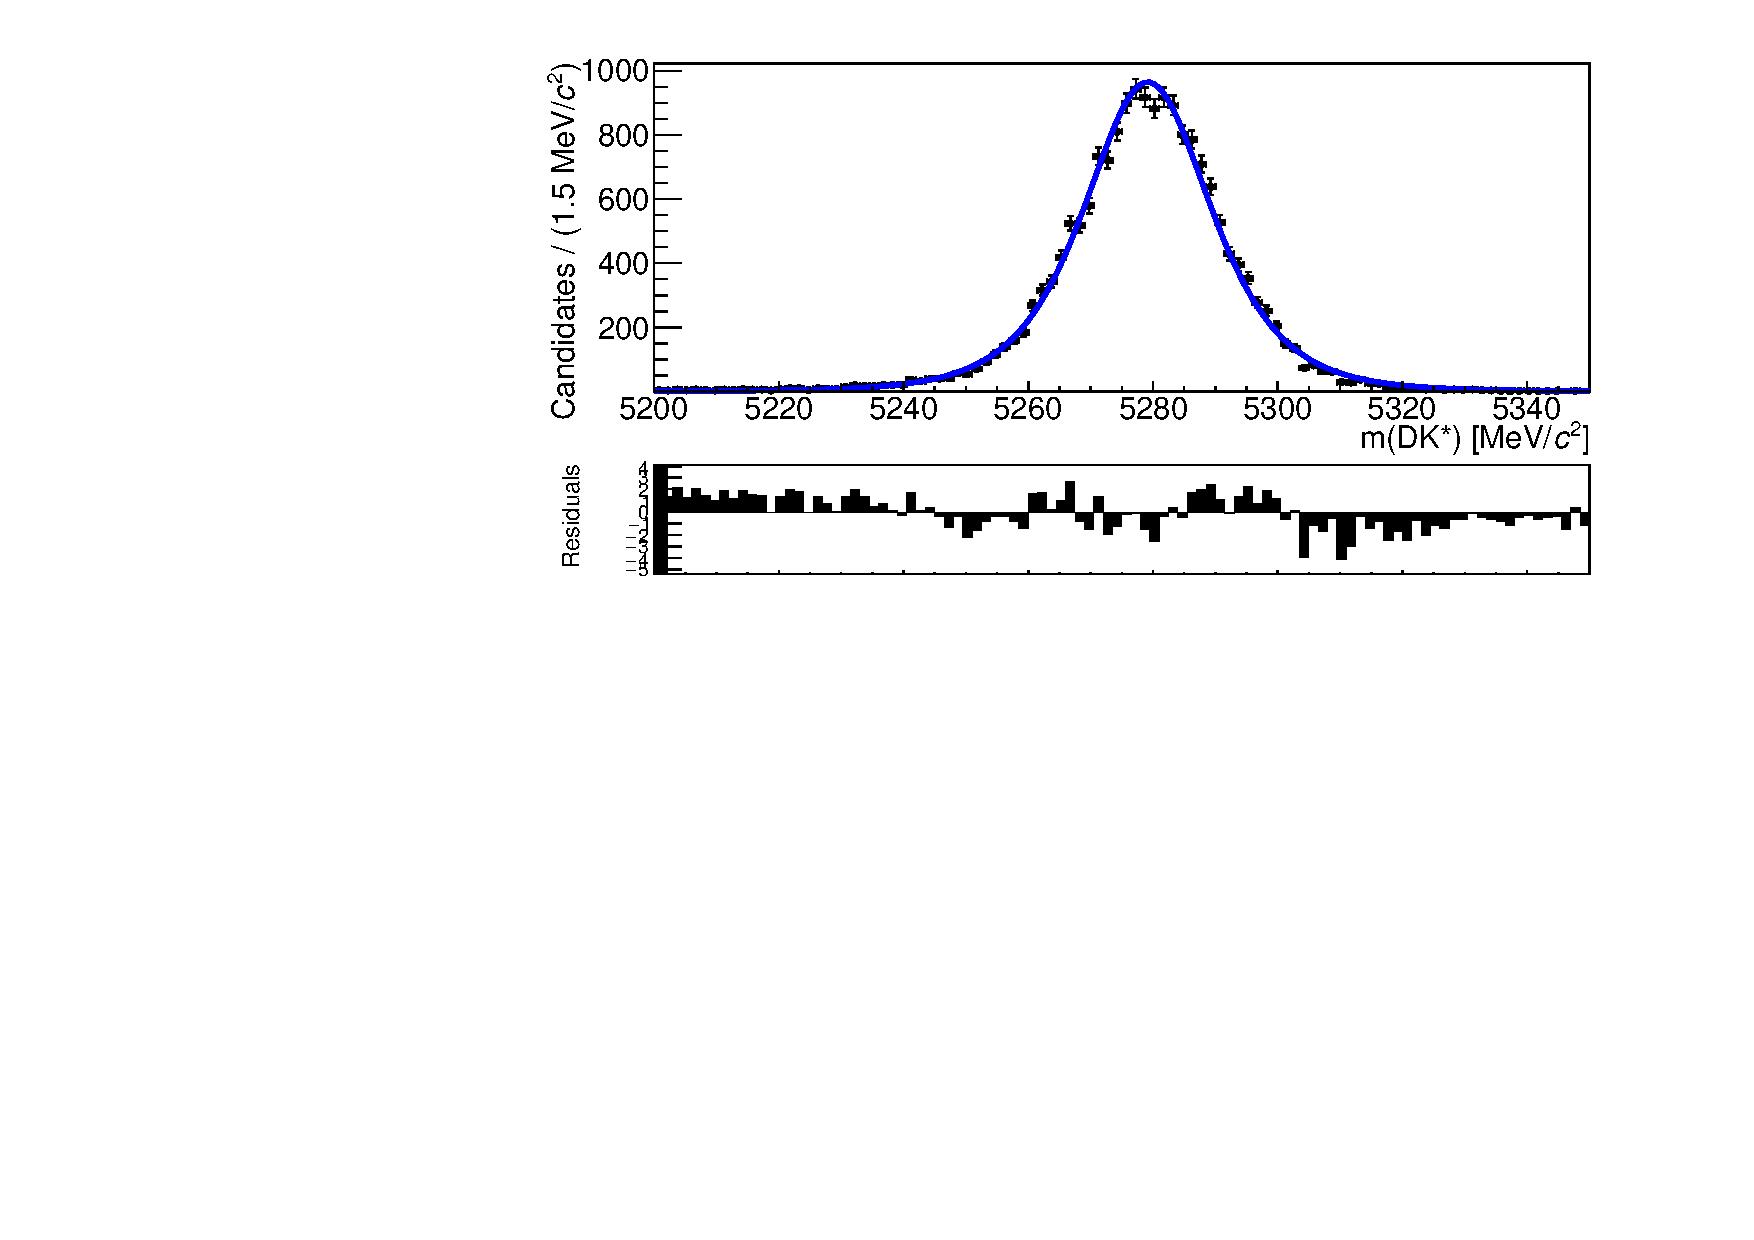
\includegraphics[width=0.7\linewidth]{figures/fitComponents/signalShape_DD_KPi_Johnson.pdf}
\caption{Maximum likelihood fit performed on a simulated signal sample of DD candidates using an alternative shape~\cite{doublejohnson}.}
\label{signalshapesys}
\end{figure}

For the width ratio and yield fraction, a systematic is assigned using Method 1, where the scale of the variation in the inputs used is the uncertainty in these values from the fits to simulated samples, as given in Table \ref{signalparameters}. The results from this method are given in the second row of Table \ref{signalshapeSystematics}. The systematic from generating an alternative distribution and that from varying the Double Crystal Ball parameters are added in quadrature to give the total signal shape systematic. The systematic calculated from the use of the alternative shape dominates the systematic uncertainty relating to the signal shape for most of the \CP observables.

\begin{table}[h]
\centering
\resizebox{\textwidth}{!}{
\begin{tabular}{ccccccccc}
\hline
& $A_{K\pi}$ & $A_{KK}$ & $A_{\pi\pi}$ & $R_{KK}$ & $R_{\pi\pi}$ & $R^+_{K\pi}$ & $R^-_{K\pi}$ \\
\hline
Alternative shape & $1.1 \times 10^{-3}$ & $2.9 \times 10^{-3}$ & $1.1 \times 10^{-2}$ & $3.0 \times 10^{-3}$ & $2.6 \times 10^{-2}$ & $1.0 \times 10^{-3}$ & $1.3 \times 10^{-3}$ \\
Vary parameters & $2.3 \times 10^{-4}$ & $1.1 \times 10^{-3}$ & $1.4 \times 10^{-3}$ & $5.9 \times 10^{-4}$ & $4.4 \times 10^{-3}$ & $2.2 \times 10^{-4}$ & $1.1 \times 10^{-4}$ \\
\hline
Total & $1.1 \times 10^{-3}$ & $3.1 \times 10^{-3}$ & $1.1 \times 10^{-2}$ & $3.0 \times 10^{-2}$ & $2.7 \times 10^{-2}$ & $1.1 \times 10^{-3}$ & $1.3 \times 10^{-3}$ \\
\hline
\end{tabular}}
\resizebox{0.78\textwidth}{!}{
\begin{tabular}{cccccc}
\hline
& $A_{K\pi\pi\pi}$ & $A_{\pi\pi\pi\pi}$ & $R_{\pi\pi\pi\pi}$ & $R^+_{K3\pi}$ & $R^-_{K3\pi}$ \\
\hline
Alternative shape & $1.6 \times 10^{-3}$ & $1.3 \times 10^{-3}$ & $9.8 \times 10^{-3}$ & $3.0 \times 10^{-3}$ & $3.8 \times 10^{-3}$ \\
Vary parameters & $4.7 \times 10^{-4}$ & $1.8 \times 10^{-3}$ & $2.5 \times 10^{-3}$ & $2.4 \times 10^{-4}$ & $1.2 \times 10^{-4}$ \\
\hline
Total & $1.7 \times 10^{-3}$ & $2.2 \times 10^{-3}$ & $1.0 \times 10^{-2}$ & $3.0 \times 10^{-3}$ & $3.8 \times 10^{-3}$ \\
\hline
\end{tabular}}
\caption{Summary of systematic uncertainties associated with the signal shape.}
\label{signalshapeSystematics}
\end{table}

\subsubsection{Combinatorial background}

The shape parameter of the combinatorial, $\beta$, is fixed across all \Dz modes in the \CP fit, as there is not enough data for the fit to be stable if the slopes are allowed to vary in each mode. In order to get an idea of the variation in combinatorial shape between different \Dz modes, individual maximum likelihood fits are performed to each \Dz decay mode in the high \Bm mass region (5400 - 5600 \mevcc) using an exponential function. The fits to the DD candidates are shown in Figure \ref{combinatoricDD}. Separate fits were also performed for LL candidates. The data used for these fits is \runone data with the selection applied, except for \Kstar selection and \Dz and \KS FD significance cuts. PID selection on the \Dz daughters is applied in order to be sure of accessing the difference between the different \Dz modes. The selection requirements are loosened as described in order to be left with enough data to perform a meaningful fit. The systematic is assigned using Method 2, with the combinatorial slope parameter, $\beta$, for each \Dz mode fixed to those given in Figure \ref{combinatoricDD}.

%\begin{figure}[h]
%\centering
%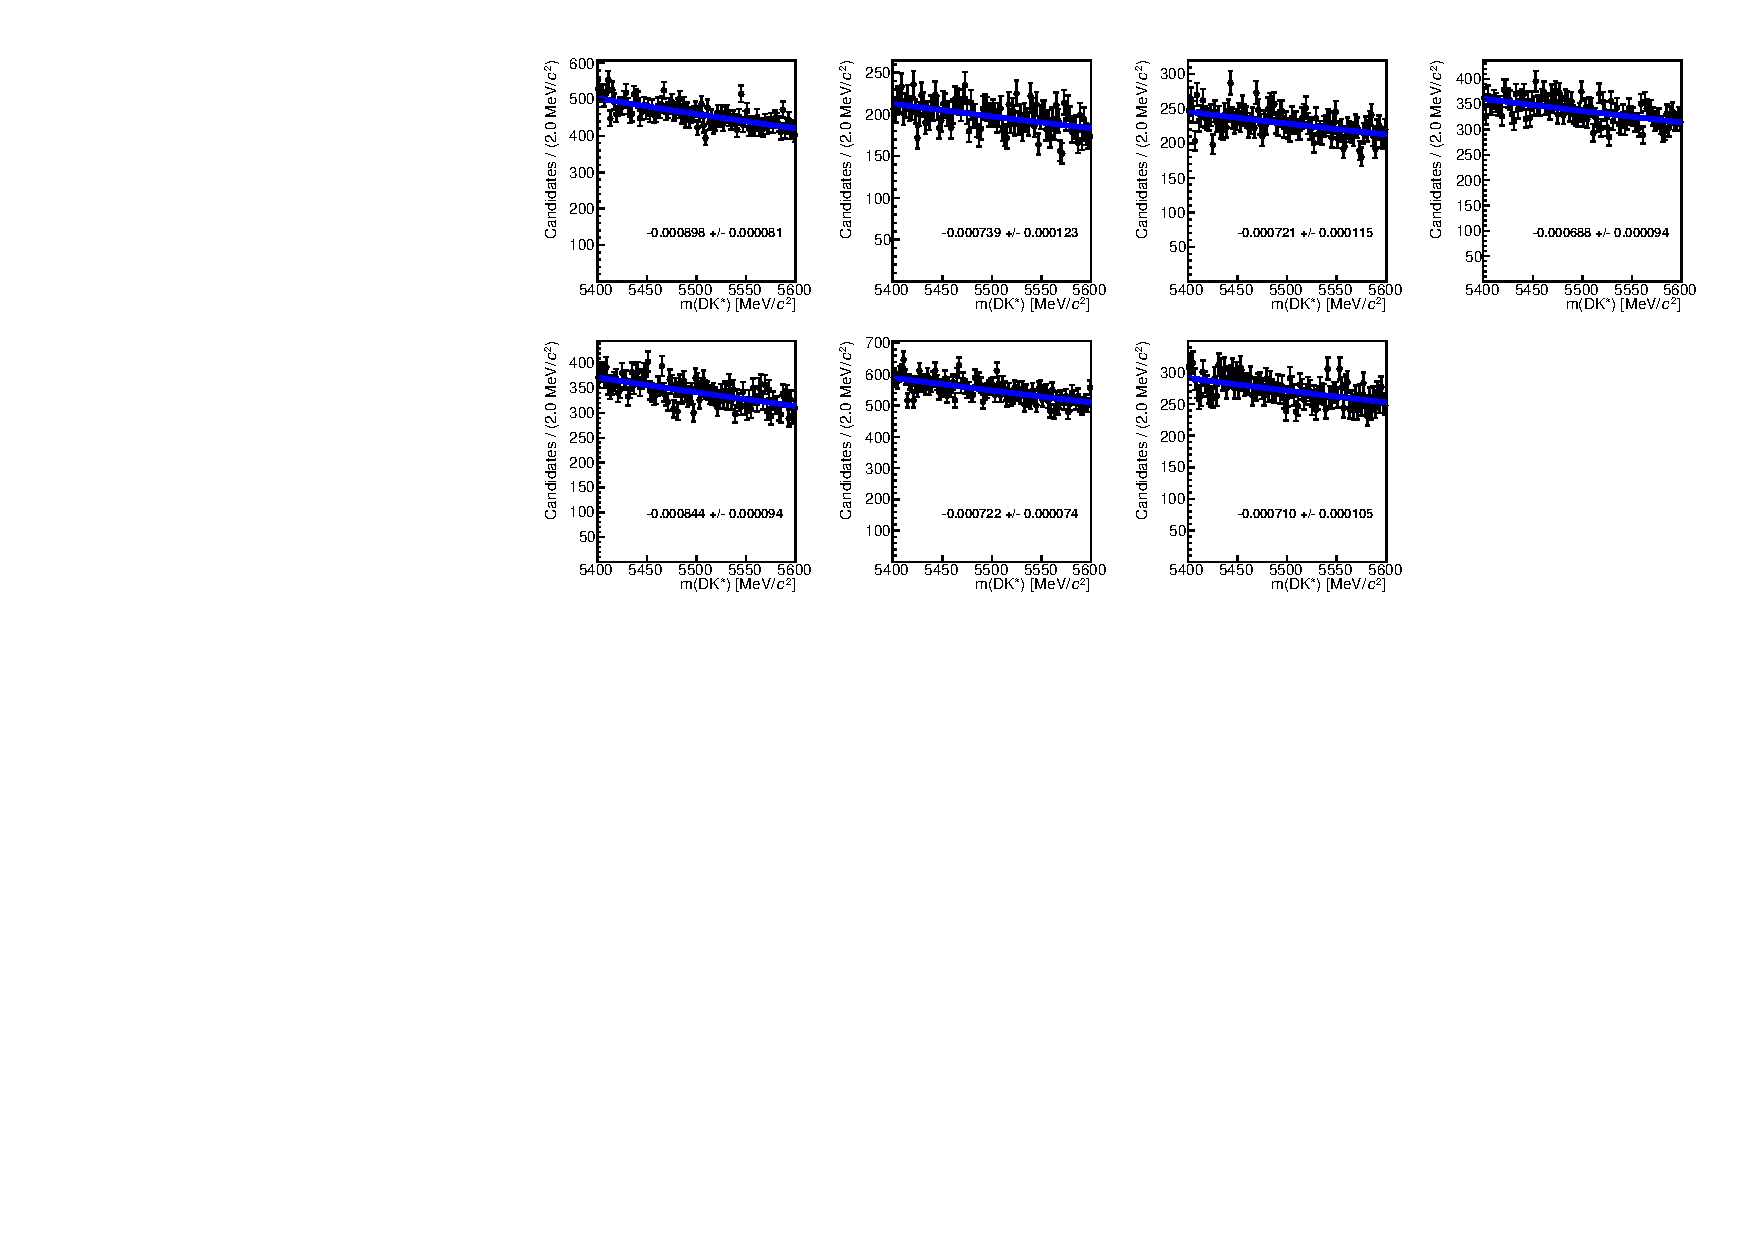
\includegraphics[width=\linewidth]{figures/fitComponents/combinatoricFits_LL.pdf}
%\caption{Maximum likelihood fits to the combinatoric background in the high \Bm mass region for LL candidates. The fitted values for the exponential slope parameter, $\beta$, are given on each plot.}
%\label{combinatoricLL}
%\end{figure}

\begin{figure}[h]
\centering
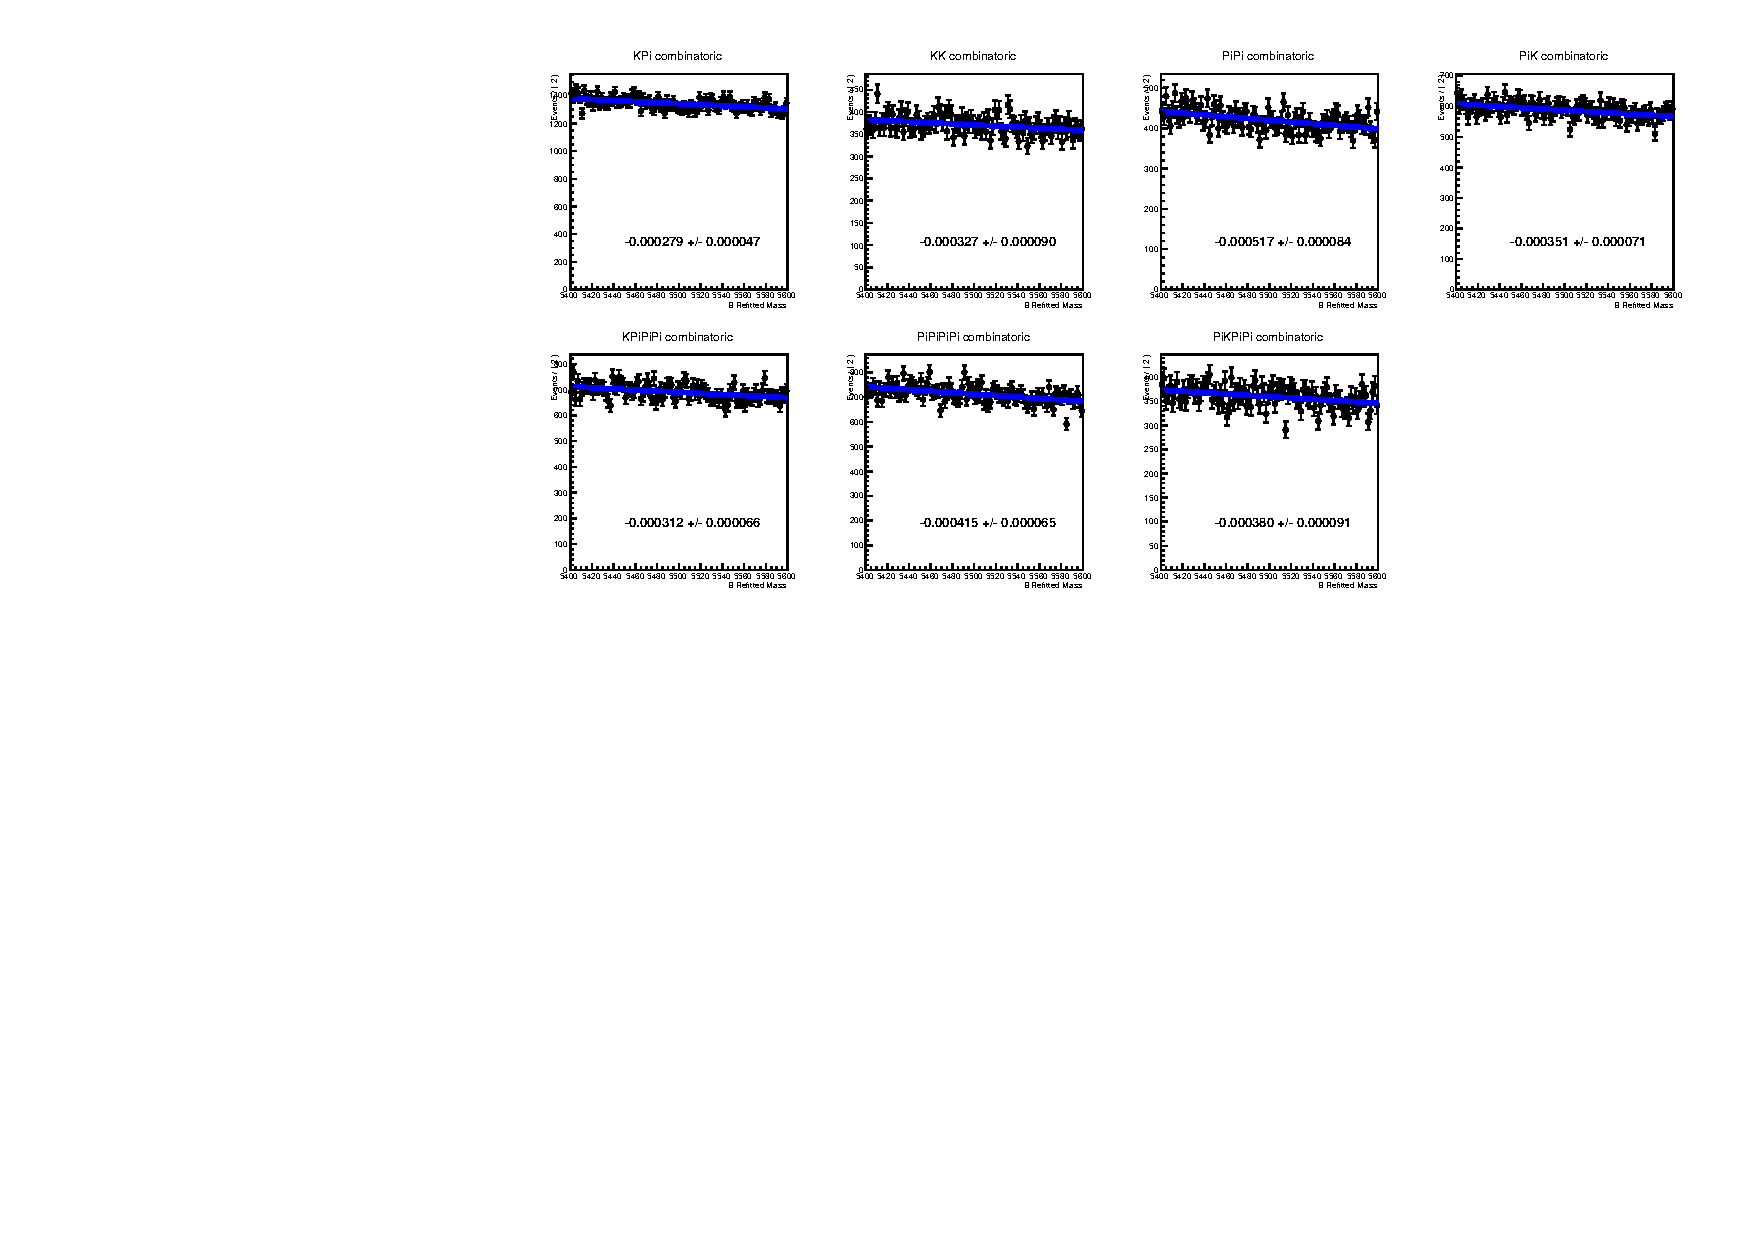
\includegraphics[width=\linewidth]{figures/fitComponents/combinatoricFits_DD.pdf}
\caption{Maximum likelihood fits to the combinatorial background in the high \Bm mass region for DD candidates. The fitted values for the exponential slope parameter, $\beta$, are given on each plot.}
\label{combinatoricDD}
\end{figure}


\subsubsection{Partially reconstructed background}
\label{sec:systematics:partreco}

The partially reconstructed decays have a completely fixed shape and yield contributing to the \CP fit, as discussed in Section \ref{sec:cpfit:partrecoyields}. Method 2 is used to assign a systematic uncertainty, making three different modifications simultaneously to the partially reconstructed region. These modifications are:

\begin{itemize}
\item The yield is increased by 20\%. The uncertainty in the yield from the fit to \kpi invariant mass is about 5\%, but this is considered to be an underestimate as other partially reconstructed low mass backgrounds, such as \decay{\Bm}{\D\Kstarm\piz}, may contribute a very small amount at low reconstructed \Bm mass, outside of the \CP fit range. This could have a slight effect on the estimate for the yield of partially reconstructed background in the \CP fit, therefore a conservative systematic of 20\% is used,
\item All partially reconstructed shapes are smeared by the difference in signal width between simulated samples and data. The width for all partially reconstructed shapes is increased by 4\% of LL bins and 5\% for DD bins,
\item A 10\% asymmetry is introduced for the partially reconstructed shapes.
\end{itemize}

\subsubsection{Charmless}

Section \ref{sec:backgrounds:charmless} shows that there is a possibility for residual charmless contribution to be present in \pipi mode. In order to estimate the associated systematic uncertainty Method 2 is used, where the yield of charmless events to be generated in the \pipi mode is drawn from a Gaussian distribution that has mean and width corresponding to the expected number of charmless events calculated in Section \ref{sec:backgrounds:charmless}. The number of events is O(1) in each of the bins for the \pipi mode. For each pseudoexperiment, the value taken from the Gaussian distribution is rounded to a whole number and randomly distributed between \Bp and \Bm, as an additional contribution to the yield in the signal region. 

\subsubsection{\boldmath \decay{\Lb}{\Lc(p\kaon\pi)\Kstarm} background}

The model for the \kk mass spectrum in \CP fit contains an additional background from \decay{\Lb}{\Lc(p\kaon\pi)\Kstarm}, as described in Section \ref{sec:backgrounds:Lb2LcKst}. The shape parameters are fixed from a maximum likelihood fit to a simulated sample of \decay{\Lb}{\Lc(p\kaon\pi)\Km}, the values of which are given in Table \ref{fitresultsLb}. The systematic uncertainty corresponding to this model component is estimated using Method 2, varying the parameters of the model according to the uncertainties in Table \ref{fitresultsLb}.

\subsubsection{\boldmath \decay{\Bs}{\Dzb\bar{K}^{*}(1410)^0} background}

The decay \decay{\Bs}{\Dzb\bar{K}^{*}(1410)^0} is considered as a background for the \pik mode, as described in Section \ref{sec:backgrounds:bs}. The shape is taken from a maximum likelihood fit to simulated events and the yield is estimated to be $2.6 \pm 2.6$ events. The systematic uncertainty corresponding to this model component is estimated using Method 2, where the generated yield is drawn from a Gaussian distribution that has mean of $2.6$ and a width of $2.6$.

\subsection{Results of systematic uncertainties}

Table \ref{systematics} summarises the systematic uncertainties for each of the different sources discussed in this section. If the systematic uncertainty was found to be over two orders of magnitude smaller than the statistical uncertainty then a value of zero is given. All systematic uncertainties are smaller than the corresponding statistical uncertainty. Systematics from simulation efficiencies and branching ratios mainly affects \Rkk and \Rpipi. Production and detection asymmetry systematics contribute to \Akpi, \Akk and \Apipi. Systematic uncertainty from PID efficiencies only have a very small contribution to the systematic uncertainty. PID asymmetry corrections are found to be negligible; they do not contribute enough to be included in Table \ref{systematics}. The signal shape systematic has a significant effect on the uncertainty for all the \CP observables. 

\begin{sidewaystable}[htbp]
\centering
{\footnotesize
\begin{tabular}{ccccccccccccc} 
\hline	
%\rule{0pt}{4ex}
\rule{0pt}{2.5ex}\rule[-1.2ex]{0pt}{0ex} & $A_{K\pi}$ & $A_{KK}$ & $A_{\pi\pi}$ & $R_{KK}$ & $R_{\pi\pi}$ & $R^+_{K\pi}$ & $R^-_{K\pi}$ & $A_{K\pi\pi\pi}$ & $A_{\pi\pi\pi\pi}$ & $R_{\pi\pi\pi\pi}$ & $R^+_{K\pi\pi\pi}$ & $R^-_{K\pi\pi\pi}$ \\
\hline
Statistical & $0.023$ & $0.07$ & $0.13$ & $0.09$ & $0.15$ & $0.006$ & $0.004$ & $0.031$ & $0.11$ & $0.13$ & $0.008$ & $0.007$ \\
\hline
Branching fractions & $-$ & $-$ & $0.013$ & $0.001$ & $0.012$ & $-$ & $-$ & $-$ & $0.0008$ & $0.027$ & $-$ & $-$ \\
Selection efficiencies  & $-$ & $-$ & $0.007$ & $-$ & $0.006$ & $0.0002$ & $-$ & $-$ & $0.0008$ & $0.014$ & $-$ & $-$ \\
PID efficiencies  & $-$ & $-$ & $0.002$ & $-$ & $0.002$ & $-$ & $-$ & $-$ & $-$ & $0.002$ & $-$ & $-$ \\
Veto efficiencies  & $-$ & $-$ & $-$ & $-$ & $-$ & $0.0001$ & $-$ & $-$ & $-$ & $-$ & $-$ & $-$ \\
$A_{\text{prod}}$  & $0.0073$ & $0.007$ & $-$ & $0.008$ & $-$ & $-$ & $-$ & $0.0079$ & $0.0077$ & $-$ & $-$ & $-$ \\
$A_{\text{det}}$  & $0.0034$ & $0.003$ & $-$ & $0.003$ & $-$ & $0.0001$ & $-$ & $0.0034$ & $0.0030$ & $-$ & $0.0001$ & $-$ \\
Signal shape & $0.0011$ & $0.003$ & $0.011$ & $0.003$ & $0.027$ & $0.0011$ & $0.0013$ & $0.0017$ & $0.0022$ & $0.010$ & $0.0030$ & $0.0038$ \\
Combinatorial shape  & $0.0012$ & $0.003$ & $0.004$ & $0.005$ & $0.009$ & $0.0002$ & $0.0003$ & $0.0001$ & $0.0018$ & $-$ & $0.0012$ & $0.0004$ \\
Partially reconstructed shape  & $0.0007$ & $0.001$ & $0.001$ & $0.003$ & $0.005$ & $-$ & $0.0003$ & $0.0003$ & $0.0005$ & $0.002$ & $0.0008$ & $0.0001$ \\
Charmless  & $0.0008$ & $-$ & $0.002$ & $0.003$ & $0.007$ & $-$ & $0.0003$ & $0.0009$ & $0.0030$ & $0.002$ & $0.0008$ & $0.0001$ \\
\decay{\Lb}{\Lc\Kstarm} & $0.0002$ & $-$ & $0.011$ & $-$ & $0.001$ & $0.0001$ & $-$ & $-$ & $-$ & $-$ & $-$ & $-$ \\
\decay{\Bs}{\D\Kstar(1410)^0} & $-$ & $-$ & $-$ & $-$ & $-$ & $0.0005$ & $0.0001$ & $-$ & $-$ & $-$ & $-$ & $-$ \\
\hline
Total systematic & $0.0083$ & $0.009$ & $0.022$ & $0.012$ & $0.032$ & $0.0012$ & $0.0014$ & $0.0088$ & $0.0093$ & $0.032$ & $0.0034$ & $0.0038$ \\
\hline
\end{tabular}}
\caption{Summary of systematic uncertainties. Uncertainties are not shown if they are more than two orders of magnitude smaller than the statistical uncertainty.}
\label{systematics}
\end{sidewaystable}

\section{Summary of results}
\label{sec:cpfit:summary}

The final results for the \CP observables are  
\begin{alignat*}{13}
A_{K\pi} &= &\ -&0.004&\ &\pm&\ &0.023&\ &\pm&\ &0.008& \\
A_{KK} &= &&0.06&\ &\pm&\ &0.07&\ &\pm&\ &0.01& \\
A_{\pi\pi} &= &&0.15&\ &\pm&\ &0.13&\ &\pm&\ &0.02& \\
R_{KK} &= &&1.22&\ &\pm&\ &0.09&\ &\pm&\ &0.01& \\
R_{\pi\pi} &= &&1.08&\ &\pm&\ &0.14&\ &\pm&\ &0.03& \\
R^+_{K\pi} &= &&0.020&\ &\pm&\ &0.006&\ &\pm&\ &0.001& \\ 
R^-_{K\pi} &= &&0.002&\ &\pm&\ &0.004&\ &\pm&\ &0.001& \\
A_{K\pi\pi\pi} &= &\ -&0.013&\ &\pm&\ &0.031&\ &\pm&\ &0.009& \\
A_{\pi\pi\pi\pi} &= &&0.02&\ &\pm&\ &0.11&\ &\pm&\ &0.01& \\
R_{\pi\pi\pi\pi} &= &&1.08&\ &\pm&\ &0.13&\ &\pm&\ &0.03& \\
R^+_{K\pi\pi\pi} &= &&0.016&\ &\pm&\ &0.007&\ &\pm&\ &0.003& \\ 
R^-_{K\pi\pi\pi} &= &&0.006&\ &\pm&\ &0.006&\ &\pm&\ &0.004&
\end{alignat*}
where the first uncertainty is statistical and the second is systematic. The correlation matrices for the statistical and systematic uncertainties are given in Tables~\ref{statisticalcorrelations} and \ref{systematiccorrelations}, respectively. The large correlations of the systematic uncertainties are mainly due to contributions from production and detection asymmetries. Combined results from the \Kp\Km and \pip\pim decay modes, taking correlations into account, are
\begin{alignat*}{13}
R_{\CP+} &= &\ &1.18&\ &\pm&\ &0.08&\ &\pm&\ &0.01& \\
A_{\CP+} &= &\ &0.08&\ &\pm&\ &0.06&\ &\pm&\ &0.01&
\end{alignat*}
where the first uncertainty is statistical and the second is systematic. The asymmetry in the GLW modes is not statistically significant. In addition, $R^+$ and $R^-$ for the \pik and \pikpipi decay modes can be transformed into $R_{ADS} = \left(R^- + R^+\right)/2\ $and \mbox{$A_{ADS} = \left(R^- - R^+\right)/\left(R^- + R^+\right)$} in order to compare with the results from \babar~\cite{BaBarDKstar}. These results, taking correlations into account, are
\begin{alignat*}{13}
R_{ADS}^{K\pi} &= &\ &0.011&\ &\pm&\ &0.004&\ &\pm&\ &0.001& \\
A_{ADS}^{K\pi} &= &\ -&0.81&\ &\pm&\ &0.17&\ &\pm&\ &0.04& \\
R_{ADS}^{K\pi\pi\pi} &= &\ &0.011&\ &\pm&\ &0.005&\ &\pm&\ &0.003& \\
A_{ADS}^{K\pi\pi\pi} &= &\ -&0.45&\ &\pm&\ &0.21&\ &\pm&\ &0.14&
\end{alignat*}
where the first uncertainty is statistical and the second is systematic. The measured asymmetries and ratios for the two-body \Dz meson decay modes are consistent with, and more precise than, the previous measurements from \babar~\cite{BaBarDKstar}. The Wilks' theorem statistical significance~\cite{Wilks:1938dza} of the two-body and four-body ADS decay modes, is defined as,
\begin{equation}
\sqrt{-2ln\left(\frac{L_0}{L_i}\right)}
\end{equation}
where $L_0$ is the extended maximum likelihood value for the nominal \CP fit model and $L_i$ is the extended maximum likelihood value for the alternative model, which forces $R_{ADS}^{K\pi} = 0$ or $R_{ADS}^{K\pi\pi\pi} = 0$ respectively. Therefore, the more unlikely that the alternative model is correct, given the data, the higher the statistical significance. The signal significance for the two-body ADS decay mode is calculated to be 4.2$\sigma$, while for the four-body ADS decay mode it is calculated to be 2.8$\sigma$. These values do not take into account the systematic uncertainties. These results show the first evidence for \pik decays.

\begin{table}[htbp]
\centering
{\scriptsize
\resizebox{\textwidth}{!}{
\begin{tabular}{c|cccccccccccc} 
\hline 
\rule{0pt}{2.5ex}\rule[-1.2ex]{0pt}{0ex}& $A_{K\pi}$ & $A_{KK}$ & $A_{\pi\pi}$ & $R_{KK}$ & $R_{\pi\pi}$ & $R^+_{K\pi}$ & $R^-_{K\pi}$ & $A_{K\pi\pi\pi}$ & $A_{\pi\pi\pi\pi}$ & $R_{\pi\pi\pi\pi}$ & $R^+_{K\pi\pi\pi}$ & $R^-_{K\pi\pi\pi}$ \\ 
 \hline
$A_{K\pi}$ & 1 & $-$ & $-$ & $-$ & $-$ & 0.08 & $-$0.01{\color{white}$-$} & $-$ & $-$ & $-$ & $-$ & $-$ \\
$A_{KK}$ & & 1 & $-$ & $-$ & $-$ & $-$ & $-$ & $-$ & $-$ & $-$ & $-$ & $-$ \\
$A_{\pi\pi}$ & & & 1 & $-$ & $-$0.02{\color{white}$-$} & $-$ & $-$ & $-$ & $-$ & $-$ & $-$ & $-$ \\
$R_{KK}$ & & & & 1 & 0.05 & 0.02 & $-$0.01{\color{white}$-$} & $-$ & $-$ & $-$ & $-$ & $-$ \\
$R_{\pi\pi}$ & & & & & 1 & 0.03 & 0.02 & $-$ & $-$ & $-$ & $-$ & $-$ \\
$R^+_{K\pi}$ & & & & & & 1 & 0.02 & $-$ & $-$ & $-$ & $-$ & $-$ \\
$R^-_{K\pi}$ & & & & & & & 1 & $-$ & $-$ & $-$ & $-$ & $-$ \\
$A_{K\pi\pi\pi}$ & & & & & & & & 1 & $-$ & $-$ & 0.07 & $-$0.03{\color{white}$-$} \\
$A_{\pi\pi\pi\pi}$ & & & & & & & & & 1 & 0.01 & $-$ & $-$ \\
$R_{\pi\pi\pi\pi}$ & & & & & & & & & & 1 & 0.04 & 0.04 \\
$R^+_{K\pi\pi\pi}$ & & & & & & & & & & & 1 & 0.03 \\
\rule[-1.2ex]{0pt}{0ex}$R^-_{K\pi\pi\pi}$ & & & & & & & & & & & & 1 \\
\hline 
\end{tabular}}}
\caption{Correlation matrix of the statistical uncertainties for the twelve physics observables from the simultaneous fit to data. Only half of the symmetric matrix is shown.}
\label{statisticalcorrelations}
\end{table}

\begin{table}[htbp]
\centering
{\scriptsize
\resizebox{\textwidth}{!}{
\begin{tabular}{c|cccccccccccc} 
\hline 
\rule{0pt}{2.5ex}\rule[-1.2ex]{0pt}{0ex}& $A_{K\pi}$ & $A_{KK}$ & $A_{\pi\pi}$ & $R_{KK}$ & $R_{\pi\pi}$ & $R^+_{K\pi}$ & $R^-_{K\pi}$ & $A_{K\pi\pi\pi}$ & $A_{\pi\pi\pi\pi}$ & $R_{\pi\pi\pi\pi}$ & $R^+_{K\pi\pi\pi}$ & $R^-_{K\pi\pi\pi}$ \\ 
 \hline
$A_{K\pi}$ & 1 & 0.82 & $-$ & 0.72 & $-$ & 0.01 & $-$0.02{\color{white}$-$} & 0.94 & 0.84 & $-$ & $-$0.01{\color{white}$-$} & $-$ \\
$A_{KK}$ & & 1 & $-$0.04{\color{white}$-$} & 0.65 & 0.02 & 0.01 & $-$0.02{\color{white}$-$} & 0.83 & 0.77 & $-$ & $-$ & $-$\\
$A_{\pi\pi}$ & & & 1 & $-$ & $-$ & 0.05 & 0.03 & $-$0.01{\color{white}$-$} & $-$ & $-$0.01{\color{white}$-$} & $-$0.01{\color{white}$-$} & $-$0.01{\color{white}$-$} \\
$R_{KK}$ & & & & 1 & $-$0.03{\color{white}$-$} & $-$ & $-$0.02{\color{white}$-$} & 0.72 & 0.68 & $-$ & $-$ & 0.01 \\
$R_{\pi\pi}$ & & & & & 1 & 0.06 & 0.08 & $-$0.01{\color{white}$-$} & $-$ & $-$0.01{\color{white}$-$} & $-$0.02{\color{white}$-$} & 0.01 \\
$R^+_{K\pi}$ & & & & & & 1 & 0.08 & $-$0.01{\color{white}$-$} & $-$ & $-$ & $-$0.01{\color{white}$-$} & $-$0.01{\color{white}$-$} \\
$R^-_{K\pi}$ & & & & & &  & 1 & $-$0.01{\color{white}$-$} & $-$0.01{\color{white}$-$} & $-$0.01{\color{white}$-$} & 0.01 & 0.03 \\
$A_{K\pi\pi\pi}$ & & & & & & & & 1 & 0.84 & $-$ & $-$0.01{\color{white}$-$} & $-$0.02{\color{white}$-$} \\
$A_{\pi\pi\pi\pi}$ & & & & & & & & & 1 & 0.03 & 0.01 & $-$ \\
$R_{\pi\pi\pi\pi}$ & & & & & & & & & & 1 & 0.01 & $-$0.01{\color{white}$-$} \\
$R^+_{K\pi\pi\pi}$ & & & & & & & & & & & 1 & 0.05 \\
\rule[-1.2ex]{0pt}{0ex}$R^-_{K\pi\pi\pi}$ & & & & & & & & & & & & 1 \\
\hline 
\end{tabular}}}
\caption{Correlation matrix of the systematic uncertainties for the twelve physics observables from the simultaneous fit to data. Only half of the symmetric matrix is shown.}
\label{systematiccorrelations}
\end{table}


\clearpage

